\documentclass[twoside]{book}

% Packages required by doxygen
\usepackage{fixltx2e}
\usepackage{calc}
\usepackage{doxygen}
\usepackage[export]{adjustbox} % also loads graphicx
\usepackage{graphicx}
\usepackage[utf8]{inputenc}
\usepackage{makeidx}
\usepackage{multicol}
\usepackage{multirow}
\PassOptionsToPackage{warn}{textcomp}
\usepackage{textcomp}
\usepackage[nointegrals]{wasysym}
\usepackage[table]{xcolor}

% Font selection
\usepackage[T1]{fontenc}
\usepackage[scaled=.90]{helvet}
\usepackage{courier}
\usepackage{amssymb}
\usepackage{sectsty}
\renewcommand{\familydefault}{\sfdefault}
\allsectionsfont{%
  \fontseries{bc}\selectfont%
  \color{darkgray}%
}
\renewcommand{\DoxyLabelFont}{%
  \fontseries{bc}\selectfont%
  \color{darkgray}%
}
\newcommand{\+}{\discretionary{\mbox{\scriptsize$\hookleftarrow$}}{}{}}

% Page & text layout
\usepackage{geometry}
\geometry{%
  a4paper,%
  top=2.5cm,%
  bottom=2.5cm,%
  left=2.5cm,%
  right=2.5cm%
}
\tolerance=750
\hfuzz=15pt
\hbadness=750
\setlength{\emergencystretch}{15pt}
\setlength{\parindent}{0cm}
\setlength{\parskip}{3ex plus 2ex minus 2ex}
\makeatletter
\renewcommand{\paragraph}{%
  \@startsection{paragraph}{4}{0ex}{-1.0ex}{1.0ex}{%
    \normalfont\normalsize\bfseries\SS@parafont%
  }%
}
\renewcommand{\subparagraph}{%
  \@startsection{subparagraph}{5}{0ex}{-1.0ex}{1.0ex}{%
    \normalfont\normalsize\bfseries\SS@subparafont%
  }%
}
\makeatother

% Headers & footers
\usepackage{fancyhdr}
\pagestyle{fancyplain}
\fancyhead[LE]{\fancyplain{}{\bfseries\thepage}}
\fancyhead[CE]{\fancyplain{}{}}
\fancyhead[RE]{\fancyplain{}{\bfseries\leftmark}}
\fancyhead[LO]{\fancyplain{}{\bfseries\rightmark}}
\fancyhead[CO]{\fancyplain{}{}}
\fancyhead[RO]{\fancyplain{}{\bfseries\thepage}}
\fancyfoot[LE]{\fancyplain{}{}}
\fancyfoot[CE]{\fancyplain{}{}}
\fancyfoot[RE]{\fancyplain{}{\bfseries\scriptsize Generated by Doxygen }}
\fancyfoot[LO]{\fancyplain{}{\bfseries\scriptsize Generated by Doxygen }}
\fancyfoot[CO]{\fancyplain{}{}}
\fancyfoot[RO]{\fancyplain{}{}}
\renewcommand{\footrulewidth}{0.4pt}
\renewcommand{\chaptermark}[1]{%
  \markboth{#1}{}%
}
\renewcommand{\sectionmark}[1]{%
  \markright{\thesection\ #1}%
}

% Indices & bibliography
\usepackage{natbib}
\usepackage[titles]{tocloft}
\setcounter{tocdepth}{3}
\setcounter{secnumdepth}{5}
\makeindex

% Hyperlinks (required, but should be loaded last)
\usepackage{ifpdf}
\ifpdf
  \usepackage[pdftex,pagebackref=true]{hyperref}
\else
  \usepackage[ps2pdf,pagebackref=true]{hyperref}
\fi
\hypersetup{%
  colorlinks=true,%
  linkcolor=blue,%
  citecolor=blue,%
  unicode%
}

% Custom commands
\newcommand{\clearemptydoublepage}{%
  \newpage{\pagestyle{empty}\cleardoublepage}%
}

\usepackage{caption}
\captionsetup{labelsep=space,justification=centering,font={bf},singlelinecheck=off,skip=4pt,position=top}

%===== C O N T E N T S =====

\begin{document}

% Titlepage & ToC
\hypersetup{pageanchor=false,
             bookmarksnumbered=true,
             pdfencoding=unicode
            }
\pagenumbering{alph}
\begin{titlepage}
\vspace*{7cm}
\begin{center}%
{\Large My Project }\\
\vspace*{1cm}
{\large Generated by Doxygen 1.8.14}\\
\end{center}
\end{titlepage}
\clearemptydoublepage
\pagenumbering{roman}
\tableofcontents
\clearemptydoublepage
\pagenumbering{arabic}
\hypersetup{pageanchor=true}

%--- Begin generated contents ---
\chapter{Namespace Index}
\section{Namespace List}
Here is a list of all documented namespaces with brief descriptions\+:\begin{DoxyCompactList}
\item\contentsline{section}{\mbox{\hyperlink{namespace_dr_evil}{Dr\+Evil}} }{\pageref{namespace_dr_evil}}{}
\item\contentsline{section}{\mbox{\hyperlink{namespace_dr_evil_1_1_data_structure}{Dr\+Evil.\+Data\+Structure}} }{\pageref{namespace_dr_evil_1_1_data_structure}}{}
\item\contentsline{section}{\mbox{\hyperlink{namespace_dr_evil_1_1_mechanics}{Dr\+Evil.\+Mechanics}} }{\pageref{namespace_dr_evil_1_1_mechanics}}{}
\item\contentsline{section}{\mbox{\hyperlink{namespace_dr_evil_1_1_testing}{Dr\+Evil.\+Testing}} }{\pageref{namespace_dr_evil_1_1_testing}}{}
\item\contentsline{section}{\mbox{\hyperlink{namespace_dr_evil_1_1_visuals}{Dr\+Evil.\+Visuals}} }{\pageref{namespace_dr_evil_1_1_visuals}}{}
\item\contentsline{section}{\mbox{\hyperlink{namespace_mobile_sensors}{Mobile\+Sensors}} }{\pageref{namespace_mobile_sensors}}{}
\end{DoxyCompactList}

\chapter{Hierarchical Index}
\section{Class Hierarchy}
This inheritance list is sorted roughly, but not completely, alphabetically\+:\begin{DoxyCompactList}
\item \contentsline{section}{Evil\+Action}{\pageref{class_evil_action}}{}
\item \contentsline{section}{Interaction\+Trigger}{\pageref{interface_interaction_trigger}}{}
\begin{DoxyCompactList}
\item \contentsline{section}{Object\+Trigger}{\pageref{class_object_trigger}}{}
\end{DoxyCompactList}
\item Mono\+Behaviour\begin{DoxyCompactList}
\item \contentsline{section}{Dr\+Evil.\+Data\+Structure.\+Asset\+Manager}{\pageref{class_dr_evil_1_1_data_structure_1_1_asset_manager}}{}
\item \contentsline{section}{Dr\+Evil.\+Data\+Structure.\+Game\+State}{\pageref{class_dr_evil_1_1_data_structure_1_1_game_state}}{}
\item \contentsline{section}{Dr\+Evil.\+Data\+Structure.\+Night\+Game\+Action\+Manager}{\pageref{class_dr_evil_1_1_data_structure_1_1_night_game_action_manager}}{}
\item \contentsline{section}{Dr\+Evil.\+Mechanics.\+Dialog\+Player}{\pageref{class_dr_evil_1_1_mechanics_1_1_dialog_player}}{}
\item \contentsline{section}{Dr\+Evil.\+Mechanics.\+Map\+View\+Controller}{\pageref{class_dr_evil_1_1_mechanics_1_1_map_view_controller}}{}
\item \contentsline{section}{Dr\+Evil.\+Mechanics.\+Screen\+View\+Handler}{\pageref{class_dr_evil_1_1_mechanics_1_1_screen_view_handler}}{}
\item \contentsline{section}{Dr\+Evil.\+Mechanics.\+Sound\+Controller}{\pageref{class_dr_evil_1_1_mechanics_1_1_sound_controller}}{}
\item \contentsline{section}{Dr\+Evil.\+Mechanics.\+Terror\+Level\+Controller}{\pageref{class_dr_evil_1_1_mechanics_1_1_terror_level_controller}}{}
\item \contentsline{section}{Dr\+Evil.\+Testing.\+Level\+Accomplish\+Test}{\pageref{class_dr_evil_1_1_testing_1_1_level_accomplish_test}}{}
\item \contentsline{section}{Dr\+Evil.\+Testing.\+Simulate\+Solved\+Actions}{\pageref{class_dr_evil_1_1_testing_1_1_simulate_solved_actions}}{}
\item \contentsline{section}{Dr\+Evil.\+Visuals.\+Highightable\+Object}{\pageref{class_dr_evil_1_1_visuals_1_1_highightable_object}}{}
\item \contentsline{section}{Dr\+Evil.\+Visuals.\+Interactable\+Object\+Hghlighter}{\pageref{class_dr_evil_1_1_visuals_1_1_interactable_object_hghlighter}}{}
\item \contentsline{section}{Dr\+Evil.\+Visuals.\+U\+I\+\_\+\+Graphic\+\_\+\+Rescaler}{\pageref{class_dr_evil_1_1_visuals_1_1_u_i___graphic___rescaler}}{}
\item \contentsline{section}{Dr\+Evil.\+Visuals.\+U\+I\+\_\+\+Sprite\+Animator}{\pageref{class_dr_evil_1_1_visuals_1_1_u_i___sprite_animator}}{}
\item \contentsline{section}{Dr\+Evil.\+Visuals.\+U\+I\+\_\+\+Text\+\_\+\+Rescaler}{\pageref{class_dr_evil_1_1_visuals_1_1_u_i___text___rescaler}}{}
\item \contentsline{section}{Event\+Test\+Script}{\pageref{class_event_test_script}}{}
\item \contentsline{section}{Game\+Manager}{\pageref{class_game_manager}}{}
\item \contentsline{section}{Mobile\+Sensors.\+Gyro\+Camera}{\pageref{class_mobile_sensors_1_1_gyro_camera}}{}
\item \contentsline{section}{Mobile\+Sensors.\+Mobile\+Input}{\pageref{class_mobile_sensors_1_1_mobile_input}}{}
\item \contentsline{section}{Object\+Trigger}{\pageref{class_object_trigger}}{}
\item \contentsline{section}{Screen\+Event\+Handler}{\pageref{class_screen_event_handler}}{}
\end{DoxyCompactList}
\item \contentsline{section}{Person}{\pageref{class_person}}{}
\item \contentsline{section}{Review\+Story}{\pageref{class_review_story}}{}
\item \contentsline{section}{Root\+Object}{\pageref{class_root_object}}{}
\item \contentsline{section}{Therapy\+Story}{\pageref{class_therapy_story}}{}
\item \contentsline{section}{Threshold}{\pageref{struct_threshold}}{}
\item Unity\+Event\begin{DoxyCompactList}
\item \contentsline{section}{Dr\+Evil.\+Testing.\+Level\+Is\+Over}{\pageref{class_dr_evil_1_1_testing_1_1_level_is_over}}{}
\item \contentsline{section}{Event\+Float}{\pageref{class_event_float}}{}
\item \contentsline{section}{Event\+Int}{\pageref{class_event_int}}{}
\item \contentsline{section}{Event\+Location}{\pageref{class_event_location}}{}
\item \contentsline{section}{Event\+Multi\+Touch}{\pageref{class_event_multi_touch}}{}
\item \contentsline{section}{Event\+Screen\+Position}{\pageref{class_event_screen_position}}{}
\item \contentsline{section}{Event\+String}{\pageref{class_event_string}}{}
\item \contentsline{section}{Event\+Threshold\+Level}{\pageref{class_event_threshold_level}}{}
\item \contentsline{section}{Event\+Touch}{\pageref{class_event_touch}}{}
\end{DoxyCompactList}
\item \contentsline{section}{World}{\pageref{class_world}}{}
\end{DoxyCompactList}

\chapter{Class Index}
\section{Class List}
Here are the classes, structs, unions and interfaces with brief descriptions\+:\begin{DoxyCompactList}
\item\contentsline{section}{\mbox{\hyperlink{class_dr_evil_1_1_data_structure_1_1_asset_manager}{Dr\+Evil.\+Data\+Structure.\+Asset\+Manager}} \\*A static \mbox{\hyperlink{class_dr_evil_1_1_data_structure_1_1_asset_manager}{Asset\+Manager}} for handling Data such as Audio. }{\pageref{class_dr_evil_1_1_data_structure_1_1_asset_manager}}{}
\item\contentsline{section}{\mbox{\hyperlink{class_dr_evil_1_1_mechanics_1_1_dialog_player}{Dr\+Evil.\+Mechanics.\+Dialog\+Player}} \\*This class handles all mechanics regarding diaogues }{\pageref{class_dr_evil_1_1_mechanics_1_1_dialog_player}}{}
\item\contentsline{section}{\mbox{\hyperlink{class_event_float}{Event\+Float}} }{\pageref{class_event_float}}{}
\item\contentsline{section}{\mbox{\hyperlink{class_event_int}{Event\+Int}} }{\pageref{class_event_int}}{}
\item\contentsline{section}{\mbox{\hyperlink{class_event_location}{Event\+Location}} }{\pageref{class_event_location}}{}
\item\contentsline{section}{\mbox{\hyperlink{class_event_multi_touch}{Event\+Multi\+Touch}} }{\pageref{class_event_multi_touch}}{}
\item\contentsline{section}{\mbox{\hyperlink{class_event_screen_position}{Event\+Screen\+Position}} }{\pageref{class_event_screen_position}}{}
\item\contentsline{section}{\mbox{\hyperlink{class_event_string}{Event\+String}} }{\pageref{class_event_string}}{}
\item\contentsline{section}{\mbox{\hyperlink{class_event_test_script}{Event\+Test\+Script}} \\*Just a Testing Script }{\pageref{class_event_test_script}}{}
\item\contentsline{section}{\mbox{\hyperlink{class_event_threshold_level}{Event\+Threshold\+Level}} }{\pageref{class_event_threshold_level}}{}
\item\contentsline{section}{\mbox{\hyperlink{class_event_touch}{Event\+Touch}} }{\pageref{class_event_touch}}{}
\item\contentsline{section}{\mbox{\hyperlink{class_evil_action}{Evil\+Action}} }{\pageref{class_evil_action}}{}
\item\contentsline{section}{\mbox{\hyperlink{class_game_manager}{Game\+Manager}} }{\pageref{class_game_manager}}{}
\item\contentsline{section}{\mbox{\hyperlink{class_dr_evil_1_1_data_structure_1_1_game_state}{Dr\+Evil.\+Data\+Structure.\+Game\+State}} \\*This class holds the complete datastructure of the game }{\pageref{class_dr_evil_1_1_data_structure_1_1_game_state}}{}
\item\contentsline{section}{\mbox{\hyperlink{class_mobile_sensors_1_1_gyro_camera}{Mobile\+Sensors.\+Gyro\+Camera}} \\*Applying the gyro input to the gyro camera }{\pageref{class_mobile_sensors_1_1_gyro_camera}}{}
\item\contentsline{section}{\mbox{\hyperlink{class_dr_evil_1_1_visuals_1_1_highightable_object}{Dr\+Evil.\+Visuals.\+Highightable\+Object}} \\*Simple class to highlight aimed objects }{\pageref{class_dr_evil_1_1_visuals_1_1_highightable_object}}{}
\item\contentsline{section}{\mbox{\hyperlink{class_dr_evil_1_1_visuals_1_1_interactable_object_hghlighter}{Dr\+Evil.\+Visuals.\+Interactable\+Object\+Hghlighter}} \\*Class for highlighting and updating interactable objects }{\pageref{class_dr_evil_1_1_visuals_1_1_interactable_object_hghlighter}}{}
\item\contentsline{section}{\mbox{\hyperlink{interface_interaction_trigger}{Interaction\+Trigger}} }{\pageref{interface_interaction_trigger}}{}
\item\contentsline{section}{\mbox{\hyperlink{class_dr_evil_1_1_testing_1_1_level_accomplish_test}{Dr\+Evil.\+Testing.\+Level\+Accomplish\+Test}} }{\pageref{class_dr_evil_1_1_testing_1_1_level_accomplish_test}}{}
\item\contentsline{section}{\mbox{\hyperlink{class_dr_evil_1_1_testing_1_1_level_is_over}{Dr\+Evil.\+Testing.\+Level\+Is\+Over}} }{\pageref{class_dr_evil_1_1_testing_1_1_level_is_over}}{}
\item\contentsline{section}{\mbox{\hyperlink{class_dr_evil_1_1_mechanics_1_1_map_view_controller}{Dr\+Evil.\+Mechanics.\+Map\+View\+Controller}} }{\pageref{class_dr_evil_1_1_mechanics_1_1_map_view_controller}}{}
\item\contentsline{section}{\mbox{\hyperlink{class_mobile_sensors_1_1_mobile_input}{Mobile\+Sensors.\+Mobile\+Input}} \\*This class handles A\+LL mobile inputs. This class can be accessed from everywhere }{\pageref{class_mobile_sensors_1_1_mobile_input}}{}
\item\contentsline{section}{\mbox{\hyperlink{class_dr_evil_1_1_data_structure_1_1_night_game_action_manager}{Dr\+Evil.\+Data\+Structure.\+Night\+Game\+Action\+Manager}} \\*Loading the gamedata from json and generating tasks for a level to solve from the player }{\pageref{class_dr_evil_1_1_data_structure_1_1_night_game_action_manager}}{}
\item\contentsline{section}{\mbox{\hyperlink{class_object_trigger}{Object\+Trigger}} }{\pageref{class_object_trigger}}{}
\item\contentsline{section}{\mbox{\hyperlink{class_person}{Person}} }{\pageref{class_person}}{}
\item\contentsline{section}{\mbox{\hyperlink{class_review_story}{Review\+Story}} }{\pageref{class_review_story}}{}
\item\contentsline{section}{\mbox{\hyperlink{class_root_object}{Root\+Object}} }{\pageref{class_root_object}}{}
\item\contentsline{section}{\mbox{\hyperlink{class_screen_event_handler}{Screen\+Event\+Handler}} }{\pageref{class_screen_event_handler}}{}
\item\contentsline{section}{\mbox{\hyperlink{class_dr_evil_1_1_mechanics_1_1_screen_view_handler}{Dr\+Evil.\+Mechanics.\+Screen\+View\+Handler}} \\*This class handles everything regarding scenes and views and screens. }{\pageref{class_dr_evil_1_1_mechanics_1_1_screen_view_handler}}{}
\item\contentsline{section}{\mbox{\hyperlink{class_dr_evil_1_1_testing_1_1_simulate_solved_actions}{Dr\+Evil.\+Testing.\+Simulate\+Solved\+Actions}} \\*\mbox{\hyperlink{namespace_dr_evil_1_1_testing}{Testing}} script to solve some interactions }{\pageref{class_dr_evil_1_1_testing_1_1_simulate_solved_actions}}{}
\item\contentsline{section}{\mbox{\hyperlink{class_dr_evil_1_1_mechanics_1_1_sound_controller}{Dr\+Evil.\+Mechanics.\+Sound\+Controller}} }{\pageref{class_dr_evil_1_1_mechanics_1_1_sound_controller}}{}
\item\contentsline{section}{\mbox{\hyperlink{class_dr_evil_1_1_mechanics_1_1_terror_level_controller}{Dr\+Evil.\+Mechanics.\+Terror\+Level\+Controller}} \\*This Class handles whole mechanics of the terror room }{\pageref{class_dr_evil_1_1_mechanics_1_1_terror_level_controller}}{}
\item\contentsline{section}{\mbox{\hyperlink{class_therapy_story}{Therapy\+Story}} }{\pageref{class_therapy_story}}{}
\item\contentsline{section}{\mbox{\hyperlink{struct_threshold}{Threshold}} }{\pageref{struct_threshold}}{}
\item\contentsline{section}{\mbox{\hyperlink{class_dr_evil_1_1_visuals_1_1_u_i___graphic___rescaler}{Dr\+Evil.\+Visuals.\+U\+I\+\_\+\+Graphic\+\_\+\+Rescaler}} }{\pageref{class_dr_evil_1_1_visuals_1_1_u_i___graphic___rescaler}}{}
\item\contentsline{section}{\mbox{\hyperlink{class_dr_evil_1_1_visuals_1_1_u_i___sprite_animator}{Dr\+Evil.\+Visuals.\+U\+I\+\_\+\+Sprite\+Animator}} \\*Simple class for handling animations in U\+I-\/\+Canvas }{\pageref{class_dr_evil_1_1_visuals_1_1_u_i___sprite_animator}}{}
\item\contentsline{section}{\mbox{\hyperlink{class_dr_evil_1_1_visuals_1_1_u_i___text___rescaler}{Dr\+Evil.\+Visuals.\+U\+I\+\_\+\+Text\+\_\+\+Rescaler}} \\*Simple class to rescale text font size depending on screen size }{\pageref{class_dr_evil_1_1_visuals_1_1_u_i___text___rescaler}}{}
\item\contentsline{section}{\mbox{\hyperlink{class_world}{World}} }{\pageref{class_world}}{}
\end{DoxyCompactList}

\chapter{Namespace Documentation}
\hypertarget{namespace_dr_evil}{}\section{Dr\+Evil Namespace Reference}
\label{namespace_dr_evil}\index{Dr\+Evil@{Dr\+Evil}}
\subsection*{Namespaces}
\begin{DoxyCompactItemize}
\end{DoxyCompactItemize}

\hypertarget{namespace_dr_evil_1_1_data_structure}{}\section{Dr\+Evil.\+Data\+Structure Namespace Reference}
\label{namespace_dr_evil_1_1_data_structure}\index{Dr\+Evil.\+Data\+Structure@{Dr\+Evil.\+Data\+Structure}}
\subsection*{Classes}
\begin{DoxyCompactItemize}
\item 
class \mbox{\hyperlink{class_dr_evil_1_1_data_structure_1_1_asset_manager}{Asset\+Manager}}
\begin{DoxyCompactList}\small\item\em A static \mbox{\hyperlink{class_dr_evil_1_1_data_structure_1_1_asset_manager}{Asset\+Manager}} for handling Data such as Audio. \end{DoxyCompactList}\item 
class \mbox{\hyperlink{class_dr_evil_1_1_data_structure_1_1_game_state}{Game\+State}}
\begin{DoxyCompactList}\small\item\em This class holds the complete datastructure of the game \end{DoxyCompactList}\item 
class \mbox{\hyperlink{class_dr_evil_1_1_data_structure_1_1_night_game_action_manager}{Night\+Game\+Action\+Manager}}
\begin{DoxyCompactList}\small\item\em Loading the gamedata from json and generating tasks for a level to solve from the player \end{DoxyCompactList}\end{DoxyCompactItemize}

\hypertarget{namespace_dr_evil_1_1_mechanics}{}\section{Dr\+Evil.\+Mechanics Namespace Reference}
\label{namespace_dr_evil_1_1_mechanics}\index{Dr\+Evil.\+Mechanics@{Dr\+Evil.\+Mechanics}}
\subsection*{Classes}
\begin{DoxyCompactItemize}
\item 
class \mbox{\hyperlink{class_dr_evil_1_1_mechanics_1_1_dialog_player}{Dialog\+Player}}
\begin{DoxyCompactList}\small\item\em This class handles all mechanics regarding diaogues \end{DoxyCompactList}\item 
class \mbox{\hyperlink{class_dr_evil_1_1_mechanics_1_1_map_view_controller}{Map\+View\+Controller}}
\item 
class \mbox{\hyperlink{class_dr_evil_1_1_mechanics_1_1_screen_view_handler}{Screen\+View\+Handler}}
\begin{DoxyCompactList}\small\item\em This class handles everything regarding scenes and views and screens. \end{DoxyCompactList}\item 
class \mbox{\hyperlink{class_dr_evil_1_1_mechanics_1_1_sound_controller}{Sound\+Controller}}
\item 
class \mbox{\hyperlink{class_dr_evil_1_1_mechanics_1_1_terror_level_controller}{Terror\+Level\+Controller}}
\begin{DoxyCompactList}\small\item\em This Class handles whole mechanics of the terror room \end{DoxyCompactList}\end{DoxyCompactItemize}

\hypertarget{namespace_dr_evil_1_1_testing}{}\section{Dr\+Evil.\+Testing Namespace Reference}
\label{namespace_dr_evil_1_1_testing}\index{Dr\+Evil.\+Testing@{Dr\+Evil.\+Testing}}
\subsection*{Classes}
\begin{DoxyCompactItemize}
\item 
class \mbox{\hyperlink{class_dr_evil_1_1_testing_1_1_level_accomplish_test}{Level\+Accomplish\+Test}}
\item 
class \mbox{\hyperlink{class_dr_evil_1_1_testing_1_1_level_is_over}{Level\+Is\+Over}}
\item 
class \mbox{\hyperlink{class_dr_evil_1_1_testing_1_1_simulate_solved_actions}{Simulate\+Solved\+Actions}}
\begin{DoxyCompactList}\small\item\em \mbox{\hyperlink{namespace_dr_evil_1_1_testing}{Testing}} script to solve some interactions \end{DoxyCompactList}\end{DoxyCompactItemize}

\hypertarget{namespace_dr_evil_1_1_visuals}{}\section{Dr\+Evil.\+Visuals Namespace Reference}
\label{namespace_dr_evil_1_1_visuals}\index{Dr\+Evil.\+Visuals@{Dr\+Evil.\+Visuals}}
\subsection*{Classes}
\begin{DoxyCompactItemize}
\item 
class \mbox{\hyperlink{class_dr_evil_1_1_visuals_1_1_highightable_object}{Highightable\+Object}}
\begin{DoxyCompactList}\small\item\em Simple class to highlight aimed objects \end{DoxyCompactList}\item 
class \mbox{\hyperlink{class_dr_evil_1_1_visuals_1_1_interactable_object_hghlighter}{Interactable\+Object\+Hghlighter}}
\begin{DoxyCompactList}\small\item\em Class for highlighting and updating interactable objects \end{DoxyCompactList}\item 
class \mbox{\hyperlink{class_dr_evil_1_1_visuals_1_1_u_i___graphic___rescaler}{U\+I\+\_\+\+Graphic\+\_\+\+Rescaler}}
\item 
class \mbox{\hyperlink{class_dr_evil_1_1_visuals_1_1_u_i___sprite_animator}{U\+I\+\_\+\+Sprite\+Animator}}
\begin{DoxyCompactList}\small\item\em Simple class for handling animations in U\+I-\/\+Canvas \end{DoxyCompactList}\item 
class \mbox{\hyperlink{class_dr_evil_1_1_visuals_1_1_u_i___text___rescaler}{U\+I\+\_\+\+Text\+\_\+\+Rescaler}}
\begin{DoxyCompactList}\small\item\em Simple class to rescale text font size depending on screen size \end{DoxyCompactList}\end{DoxyCompactItemize}

\hypertarget{namespace_mobile_sensors}{}\section{Mobile\+Sensors Namespace Reference}
\label{namespace_mobile_sensors}\index{Mobile\+Sensors@{Mobile\+Sensors}}
\subsection*{Classes}
\begin{DoxyCompactItemize}
\item 
class \mbox{\hyperlink{class_mobile_sensors_1_1_gyro_camera}{Gyro\+Camera}}
\begin{DoxyCompactList}\small\item\em Applying the gyro input to the gyro camera \end{DoxyCompactList}\item 
class \mbox{\hyperlink{class_mobile_sensors_1_1_mobile_input}{Mobile\+Input}}
\begin{DoxyCompactList}\small\item\em This class handles A\+LL mobile inputs. This class can be accessed from everywhere \end{DoxyCompactList}\end{DoxyCompactItemize}

\chapter{Class Documentation}
\hypertarget{class_dr_evil_1_1_data_structure_1_1_asset_manager}{}\section{Dr\+Evil.\+Data\+Structure.\+Asset\+Manager Class Reference}
\label{class_dr_evil_1_1_data_structure_1_1_asset_manager}\index{Dr\+Evil.\+Data\+Structure.\+Asset\+Manager@{Dr\+Evil.\+Data\+Structure.\+Asset\+Manager}}


A static \mbox{\hyperlink{class_dr_evil_1_1_data_structure_1_1_asset_manager}{Asset\+Manager}} for handling Data such as Audio.  


Inheritance diagram for Dr\+Evil.\+Data\+Structure.\+Asset\+Manager\+:\begin{figure}[H]
\begin{center}
\leavevmode
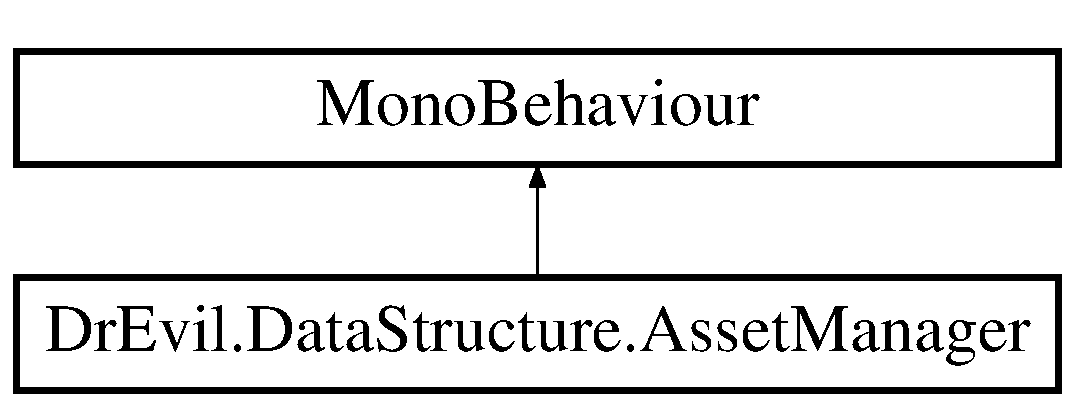
\includegraphics[height=2.000000cm]{class_dr_evil_1_1_data_structure_1_1_asset_manager}
\end{center}
\end{figure}
\subsection*{Public Attributes}
\begin{DoxyCompactItemize}
\item 
\mbox{\Hypertarget{class_dr_evil_1_1_data_structure_1_1_asset_manager_a8fb69379890323598b0b2c9c18552f6a}\label{class_dr_evil_1_1_data_structure_1_1_asset_manager_a8fb69379890323598b0b2c9c18552f6a}} 
Audio\+Clip {\bfseries scratch}
\item 
\mbox{\Hypertarget{class_dr_evil_1_1_data_structure_1_1_asset_manager_ac319353c9d6875c878ed96cdcb223ddc}\label{class_dr_evil_1_1_data_structure_1_1_asset_manager_ac319353c9d6875c878ed96cdcb223ddc}} 
Audio\+Clip {\bfseries swipe}
\item 
\mbox{\Hypertarget{class_dr_evil_1_1_data_structure_1_1_asset_manager_a00bda90d0d5c9f1d53009fbd1911973a}\label{class_dr_evil_1_1_data_structure_1_1_asset_manager_a00bda90d0d5c9f1d53009fbd1911973a}} 
Audio\+Clip {\bfseries push}
\item 
\mbox{\Hypertarget{class_dr_evil_1_1_data_structure_1_1_asset_manager_abff01e46360a0429fb5cc8a5143f224b}\label{class_dr_evil_1_1_data_structure_1_1_asset_manager_abff01e46360a0429fb5cc8a5143f224b}} 
Audio\+Clip {\bfseries touch}
\item 
\mbox{\Hypertarget{class_dr_evil_1_1_data_structure_1_1_asset_manager_a36fb40b17c5490381b55abc7b248b179}\label{class_dr_evil_1_1_data_structure_1_1_asset_manager_a36fb40b17c5490381b55abc7b248b179}} 
List$<$ Audio\+Clip $>$ {\bfseries patient\+\_\+scared\+\_\+sounds}
\item 
\mbox{\Hypertarget{class_dr_evil_1_1_data_structure_1_1_asset_manager_a3659d0e1c919ed88c3c278abc8960cd7}\label{class_dr_evil_1_1_data_structure_1_1_asset_manager_a3659d0e1c919ed88c3c278abc8960cd7}} 
List$<$ Audio\+Clip $>$ {\bfseries patient\+\_\+angry\+\_\+sounds}
\end{DoxyCompactItemize}
\subsection*{Static Public Attributes}
\begin{DoxyCompactItemize}
\item 
\mbox{\Hypertarget{class_dr_evil_1_1_data_structure_1_1_asset_manager_a17ad40765ce62d5b157668b11be83e76}\label{class_dr_evil_1_1_data_structure_1_1_asset_manager_a17ad40765ce62d5b157668b11be83e76}} 
static \mbox{\hyperlink{class_dr_evil_1_1_data_structure_1_1_asset_manager}{Asset\+Manager}} {\bfseries instance}
\end{DoxyCompactItemize}


\subsection{Detailed Description}
A static \mbox{\hyperlink{class_dr_evil_1_1_data_structure_1_1_asset_manager}{Asset\+Manager}} for handling Data such as Audio. 



The documentation for this class was generated from the following file\+:\begin{DoxyCompactItemize}
\item 
Gamejam\+Unity/\+Assets/\+Scripts/Asset\+Manager.\+cs\end{DoxyCompactItemize}

\hypertarget{class_dr_evil_1_1_mechanics_1_1_dialog_player}{}\section{Dr\+Evil.\+Mechanics.\+Dialog\+Player Class Reference}
\label{class_dr_evil_1_1_mechanics_1_1_dialog_player}\index{Dr\+Evil.\+Mechanics.\+Dialog\+Player@{Dr\+Evil.\+Mechanics.\+Dialog\+Player}}


This class handles all mechanics regarding diaogues  


Inheritance diagram for Dr\+Evil.\+Mechanics.\+Dialog\+Player\+:\begin{figure}[H]
\begin{center}
\leavevmode
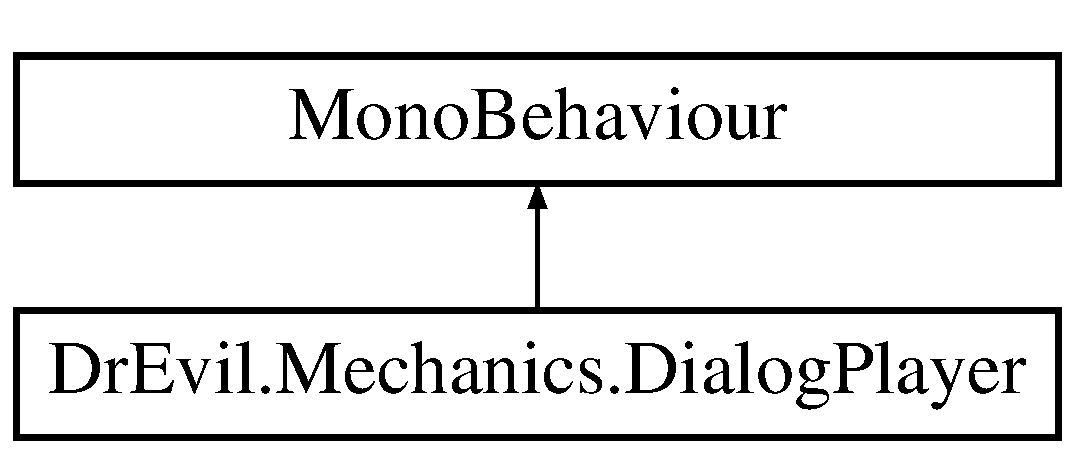
\includegraphics[height=2.000000cm]{class_dr_evil_1_1_mechanics_1_1_dialog_player}
\end{center}
\end{figure}
\subsection*{Public Member Functions}
\begin{DoxyCompactItemize}
\item 
void \mbox{\hyperlink{class_dr_evil_1_1_mechanics_1_1_dialog_player_a1d412965461502a4770f7c754f5188f0}{Play\+Story}} (\mbox{\hyperlink{class_person}{Person}} person, bool new\+Level=false)
\begin{DoxyCompactList}\small\item\em Play a given story from a level \end{DoxyCompactList}\item 
void \mbox{\hyperlink{class_dr_evil_1_1_mechanics_1_1_dialog_player_a641a18db7fcbfdbb7c052611c0d4f47d}{Initialize\+Patient\+Screen}} (\mbox{\hyperlink{class_person}{Person}} person)
\begin{DoxyCompactList}\small\item\em Set \mbox{\hyperlink{class_person}{Person}} Description and Update Sprite \end{DoxyCompactList}\item 
void \mbox{\hyperlink{class_dr_evil_1_1_mechanics_1_1_dialog_player_a00c6b192050d5dcde49caf9bd7e124b0}{Show\+Therapie\+Dialog}} ()
\begin{DoxyCompactList}\small\item\em Handling the init Dialogue for the patients \end{DoxyCompactList}\item 
I\+Enumerator \mbox{\hyperlink{class_dr_evil_1_1_mechanics_1_1_dialog_player_acd487680cd0955af518d0db6b2789813}{Dialogue\+Writer}} (string display\+Text, string actor)
\begin{DoxyCompactList}\small\item\em The Dialogue Writer for adding text over time to duialogue box \end{DoxyCompactList}\item 
void \mbox{\hyperlink{class_dr_evil_1_1_mechanics_1_1_dialog_player_ad6012eb1ba848915bfc90a73ca04c6b6}{Show\+Solved\+Dialog}} ()
\begin{DoxyCompactList}\small\item\em Handling dialogue mechanic for solved levels \end{DoxyCompactList}\item 
void \mbox{\hyperlink{class_dr_evil_1_1_mechanics_1_1_dialog_player_a38669bb0c15607e64dca7741052f9c6e}{Show\+Partially\+Solved\+Dialog}} ()
\begin{DoxyCompactList}\small\item\em handling the dialogue for partially solved levels \end{DoxyCompactList}\end{DoxyCompactItemize}
\subsection*{Public Attributes}
\begin{DoxyCompactItemize}
\item 
\mbox{\Hypertarget{class_dr_evil_1_1_mechanics_1_1_dialog_player_a983dd1c3719ee79abbc99a36cae653b5}\label{class_dr_evil_1_1_mechanics_1_1_dialog_player_a983dd1c3719ee79abbc99a36cae653b5}} 
Game\+Object {\bfseries Therapy\+Screen\+Game\+Object}
\item 
\mbox{\Hypertarget{class_dr_evil_1_1_mechanics_1_1_dialog_player_aa7097e406e357dc86f74ee62079f48ba}\label{class_dr_evil_1_1_mechanics_1_1_dialog_player_aa7097e406e357dc86f74ee62079f48ba}} 
Game\+Object {\bfseries Dialog\+Field}
\item 
\mbox{\Hypertarget{class_dr_evil_1_1_mechanics_1_1_dialog_player_af2eaeda0b3d7d5e46f292cf7f8e96b4e}\label{class_dr_evil_1_1_mechanics_1_1_dialog_player_af2eaeda0b3d7d5e46f292cf7f8e96b4e}} 
Text {\bfseries dialog\+Fieldtext}
\item 
\mbox{\Hypertarget{class_dr_evil_1_1_mechanics_1_1_dialog_player_a8c82e3930a1adcc2592541ec90213993}\label{class_dr_evil_1_1_mechanics_1_1_dialog_player_a8c82e3930a1adcc2592541ec90213993}} 
Game\+Object {\bfseries Evil\+Screen\+Game\+Object}
\item 
\mbox{\Hypertarget{class_dr_evil_1_1_mechanics_1_1_dialog_player_a7af415ffaae175b0efe910e017fa6755}\label{class_dr_evil_1_1_mechanics_1_1_dialog_player_a7af415ffaae175b0efe910e017fa6755}} 
Game\+Object {\bfseries Patient\+Screen\+Game\+Object}
\item 
\mbox{\Hypertarget{class_dr_evil_1_1_mechanics_1_1_dialog_player_a7e522a7e2711ef5f0e15bd98fcdefb51}\label{class_dr_evil_1_1_mechanics_1_1_dialog_player_a7e522a7e2711ef5f0e15bd98fcdefb51}} 
Image {\bfseries Patient\+Sprite}
\item 
\mbox{\Hypertarget{class_dr_evil_1_1_mechanics_1_1_dialog_player_a856932c49138c2d383c1aeec0f33eb2d}\label{class_dr_evil_1_1_mechanics_1_1_dialog_player_a856932c49138c2d383c1aeec0f33eb2d}} 
Text {\bfseries Patient\+Bio\+Info\+Text}
\item 
\mbox{\Hypertarget{class_dr_evil_1_1_mechanics_1_1_dialog_player_a99d0271b454ebfbf3096d41567cc5e1f}\label{class_dr_evil_1_1_mechanics_1_1_dialog_player_a99d0271b454ebfbf3096d41567cc5e1f}} 
Button {\bfseries Next\+Dialog\+Button}
\end{DoxyCompactItemize}


\subsection{Detailed Description}
This class handles all mechanics regarding diaogues 



\subsection{Member Function Documentation}
\mbox{\Hypertarget{class_dr_evil_1_1_mechanics_1_1_dialog_player_acd487680cd0955af518d0db6b2789813}\label{class_dr_evil_1_1_mechanics_1_1_dialog_player_acd487680cd0955af518d0db6b2789813}} 
\index{Dr\+Evil\+::\+Mechanics\+::\+Dialog\+Player@{Dr\+Evil\+::\+Mechanics\+::\+Dialog\+Player}!Dialogue\+Writer@{Dialogue\+Writer}}
\index{Dialogue\+Writer@{Dialogue\+Writer}!Dr\+Evil\+::\+Mechanics\+::\+Dialog\+Player@{Dr\+Evil\+::\+Mechanics\+::\+Dialog\+Player}}
\subsubsection{\texorpdfstring{Dialogue\+Writer()}{DialogueWriter()}}
{\footnotesize\ttfamily I\+Enumerator Dr\+Evil.\+Mechanics.\+Dialog\+Player.\+Dialogue\+Writer (\begin{DoxyParamCaption}\item[{string}]{display\+Text,  }\item[{string}]{actor }\end{DoxyParamCaption})\hspace{0.3cm}{\ttfamily [inline]}}



The Dialogue Writer for adding text over time to duialogue box 


\begin{DoxyParams}{Parameters}
{\em display\+Text} & \\
\hline
{\em actor} & \\
\hline
\end{DoxyParams}
\begin{DoxyReturn}{Returns}

\end{DoxyReturn}
\mbox{\Hypertarget{class_dr_evil_1_1_mechanics_1_1_dialog_player_a641a18db7fcbfdbb7c052611c0d4f47d}\label{class_dr_evil_1_1_mechanics_1_1_dialog_player_a641a18db7fcbfdbb7c052611c0d4f47d}} 
\index{Dr\+Evil\+::\+Mechanics\+::\+Dialog\+Player@{Dr\+Evil\+::\+Mechanics\+::\+Dialog\+Player}!Initialize\+Patient\+Screen@{Initialize\+Patient\+Screen}}
\index{Initialize\+Patient\+Screen@{Initialize\+Patient\+Screen}!Dr\+Evil\+::\+Mechanics\+::\+Dialog\+Player@{Dr\+Evil\+::\+Mechanics\+::\+Dialog\+Player}}
\subsubsection{\texorpdfstring{Initialize\+Patient\+Screen()}{InitializePatientScreen()}}
{\footnotesize\ttfamily void Dr\+Evil.\+Mechanics.\+Dialog\+Player.\+Initialize\+Patient\+Screen (\begin{DoxyParamCaption}\item[{\mbox{\hyperlink{class_person}{Person}}}]{person }\end{DoxyParamCaption})\hspace{0.3cm}{\ttfamily [inline]}}



Set \mbox{\hyperlink{class_person}{Person}} Description and Update Sprite 


\begin{DoxyParams}{Parameters}
{\em person} & \\
\hline
\end{DoxyParams}
\mbox{\Hypertarget{class_dr_evil_1_1_mechanics_1_1_dialog_player_a1d412965461502a4770f7c754f5188f0}\label{class_dr_evil_1_1_mechanics_1_1_dialog_player_a1d412965461502a4770f7c754f5188f0}} 
\index{Dr\+Evil\+::\+Mechanics\+::\+Dialog\+Player@{Dr\+Evil\+::\+Mechanics\+::\+Dialog\+Player}!Play\+Story@{Play\+Story}}
\index{Play\+Story@{Play\+Story}!Dr\+Evil\+::\+Mechanics\+::\+Dialog\+Player@{Dr\+Evil\+::\+Mechanics\+::\+Dialog\+Player}}
\subsubsection{\texorpdfstring{Play\+Story()}{PlayStory()}}
{\footnotesize\ttfamily void Dr\+Evil.\+Mechanics.\+Dialog\+Player.\+Play\+Story (\begin{DoxyParamCaption}\item[{\mbox{\hyperlink{class_person}{Person}}}]{person,  }\item[{bool}]{new\+Level = {\ttfamily false} }\end{DoxyParamCaption})\hspace{0.3cm}{\ttfamily [inline]}}



Play a given story from a level 


\begin{DoxyParams}{Parameters}
{\em person} & \\
\hline
{\em new\+Level} & \\
\hline
\end{DoxyParams}
\mbox{\Hypertarget{class_dr_evil_1_1_mechanics_1_1_dialog_player_a38669bb0c15607e64dca7741052f9c6e}\label{class_dr_evil_1_1_mechanics_1_1_dialog_player_a38669bb0c15607e64dca7741052f9c6e}} 
\index{Dr\+Evil\+::\+Mechanics\+::\+Dialog\+Player@{Dr\+Evil\+::\+Mechanics\+::\+Dialog\+Player}!Show\+Partially\+Solved\+Dialog@{Show\+Partially\+Solved\+Dialog}}
\index{Show\+Partially\+Solved\+Dialog@{Show\+Partially\+Solved\+Dialog}!Dr\+Evil\+::\+Mechanics\+::\+Dialog\+Player@{Dr\+Evil\+::\+Mechanics\+::\+Dialog\+Player}}
\subsubsection{\texorpdfstring{Show\+Partially\+Solved\+Dialog()}{ShowPartiallySolvedDialog()}}
{\footnotesize\ttfamily void Dr\+Evil.\+Mechanics.\+Dialog\+Player.\+Show\+Partially\+Solved\+Dialog (\begin{DoxyParamCaption}{ }\end{DoxyParamCaption})\hspace{0.3cm}{\ttfamily [inline]}}



handling the dialogue for partially solved levels 

\mbox{\Hypertarget{class_dr_evil_1_1_mechanics_1_1_dialog_player_ad6012eb1ba848915bfc90a73ca04c6b6}\label{class_dr_evil_1_1_mechanics_1_1_dialog_player_ad6012eb1ba848915bfc90a73ca04c6b6}} 
\index{Dr\+Evil\+::\+Mechanics\+::\+Dialog\+Player@{Dr\+Evil\+::\+Mechanics\+::\+Dialog\+Player}!Show\+Solved\+Dialog@{Show\+Solved\+Dialog}}
\index{Show\+Solved\+Dialog@{Show\+Solved\+Dialog}!Dr\+Evil\+::\+Mechanics\+::\+Dialog\+Player@{Dr\+Evil\+::\+Mechanics\+::\+Dialog\+Player}}
\subsubsection{\texorpdfstring{Show\+Solved\+Dialog()}{ShowSolvedDialog()}}
{\footnotesize\ttfamily void Dr\+Evil.\+Mechanics.\+Dialog\+Player.\+Show\+Solved\+Dialog (\begin{DoxyParamCaption}{ }\end{DoxyParamCaption})\hspace{0.3cm}{\ttfamily [inline]}}



Handling dialogue mechanic for solved levels 

\mbox{\Hypertarget{class_dr_evil_1_1_mechanics_1_1_dialog_player_a00c6b192050d5dcde49caf9bd7e124b0}\label{class_dr_evil_1_1_mechanics_1_1_dialog_player_a00c6b192050d5dcde49caf9bd7e124b0}} 
\index{Dr\+Evil\+::\+Mechanics\+::\+Dialog\+Player@{Dr\+Evil\+::\+Mechanics\+::\+Dialog\+Player}!Show\+Therapie\+Dialog@{Show\+Therapie\+Dialog}}
\index{Show\+Therapie\+Dialog@{Show\+Therapie\+Dialog}!Dr\+Evil\+::\+Mechanics\+::\+Dialog\+Player@{Dr\+Evil\+::\+Mechanics\+::\+Dialog\+Player}}
\subsubsection{\texorpdfstring{Show\+Therapie\+Dialog()}{ShowTherapieDialog()}}
{\footnotesize\ttfamily void Dr\+Evil.\+Mechanics.\+Dialog\+Player.\+Show\+Therapie\+Dialog (\begin{DoxyParamCaption}{ }\end{DoxyParamCaption})\hspace{0.3cm}{\ttfamily [inline]}}



Handling the init Dialogue for the patients 



The documentation for this class was generated from the following file\+:\begin{DoxyCompactItemize}
\item 
Gamejam\+Unity/\+Assets/\+Scripts/Dialog\+Player.\+cs\end{DoxyCompactItemize}

\hypertarget{class_event_float}{}\section{Event\+Float Class Reference}
\label{class_event_float}\index{Event\+Float@{Event\+Float}}
Inheritance diagram for Event\+Float\+:\begin{figure}[H]
\begin{center}
\leavevmode
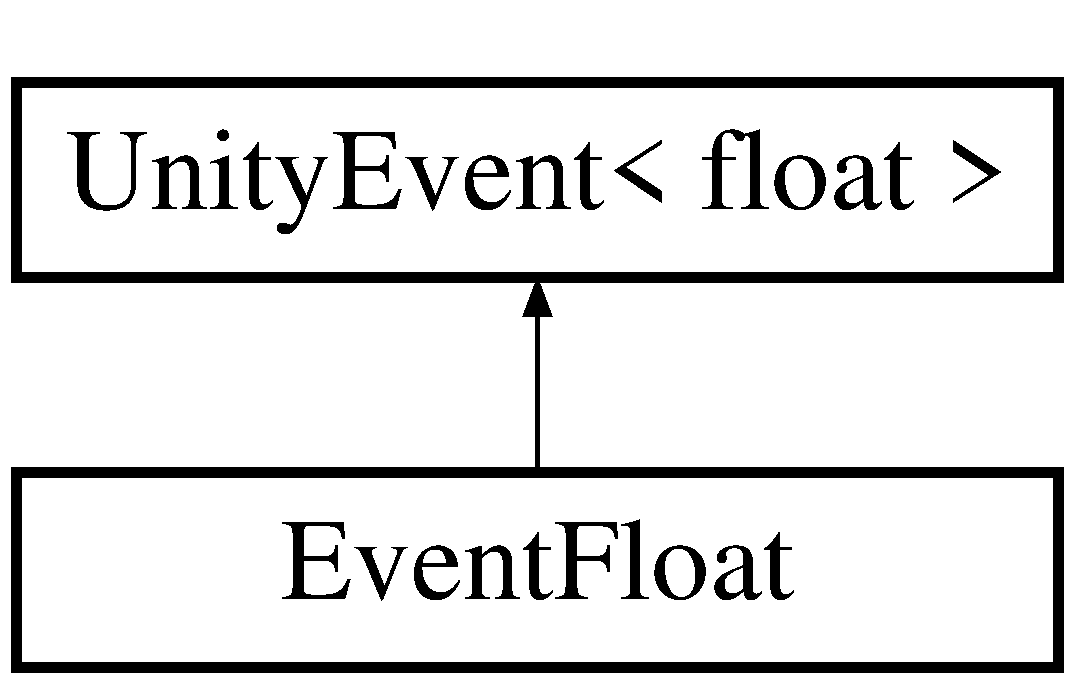
\includegraphics[height=2.000000cm]{class_event_float}
\end{center}
\end{figure}


The documentation for this class was generated from the following file\+:\begin{DoxyCompactItemize}
\item 
Gamejam\+Unity/\+Assets/\+Scripts/Mobile\+Input.\+cs\end{DoxyCompactItemize}

\hypertarget{class_event_int}{}\section{Event\+Int Class Reference}
\label{class_event_int}\index{Event\+Int@{Event\+Int}}
Inheritance diagram for Event\+Int\+:\begin{figure}[H]
\begin{center}
\leavevmode
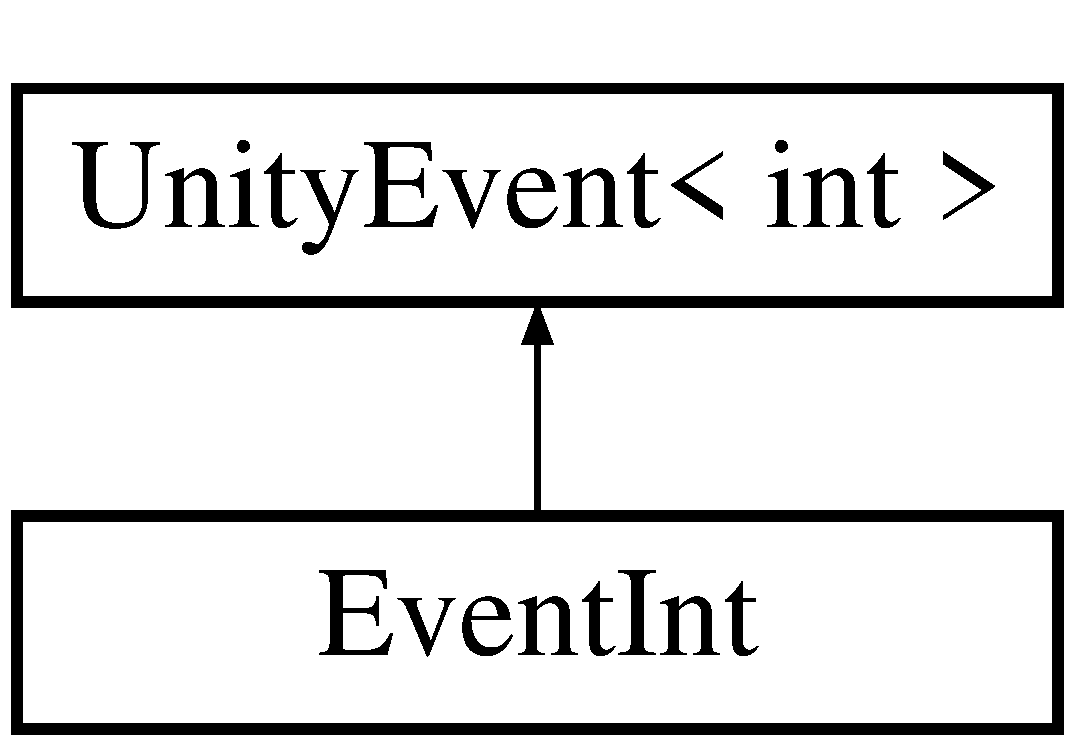
\includegraphics[height=2.000000cm]{class_event_int}
\end{center}
\end{figure}


The documentation for this class was generated from the following file\+:\begin{DoxyCompactItemize}
\item 
Gamejam\+Unity/\+Assets/\+Scripts/Mobile\+Input.\+cs\end{DoxyCompactItemize}

\hypertarget{class_event_location}{}\section{Event\+Location Class Reference}
\label{class_event_location}\index{Event\+Location@{Event\+Location}}
Inheritance diagram for Event\+Location\+:\begin{figure}[H]
\begin{center}
\leavevmode
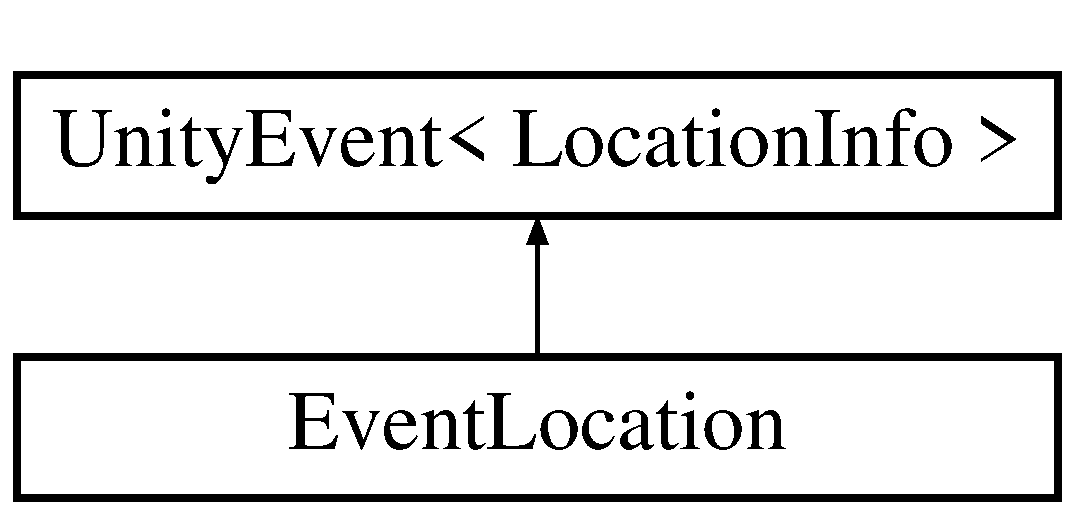
\includegraphics[height=2.000000cm]{class_event_location}
\end{center}
\end{figure}


The documentation for this class was generated from the following file\+:\begin{DoxyCompactItemize}
\item 
Gamejam\+Unity/\+Assets/\+Scripts/Mobile\+Input.\+cs\end{DoxyCompactItemize}

\hypertarget{class_event_multi_touch}{}\section{Event\+Multi\+Touch Class Reference}
\label{class_event_multi_touch}\index{Event\+Multi\+Touch@{Event\+Multi\+Touch}}
Inheritance diagram for Event\+Multi\+Touch\+:\begin{figure}[H]
\begin{center}
\leavevmode
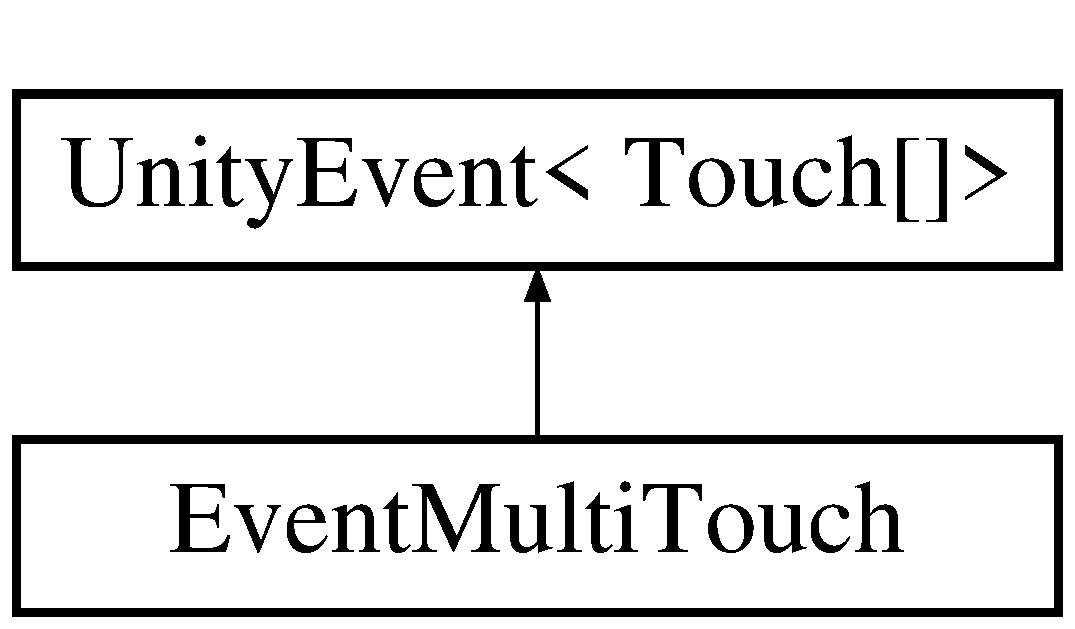
\includegraphics[height=2.000000cm]{class_event_multi_touch}
\end{center}
\end{figure}


The documentation for this class was generated from the following file\+:\begin{DoxyCompactItemize}
\item 
Gamejam\+Unity/\+Assets/\+Scripts/Mobile\+Input.\+cs\end{DoxyCompactItemize}

\hypertarget{class_event_screen_position}{}\section{Event\+Screen\+Position Class Reference}
\label{class_event_screen_position}\index{Event\+Screen\+Position@{Event\+Screen\+Position}}
Inheritance diagram for Event\+Screen\+Position\+:\begin{figure}[H]
\begin{center}
\leavevmode
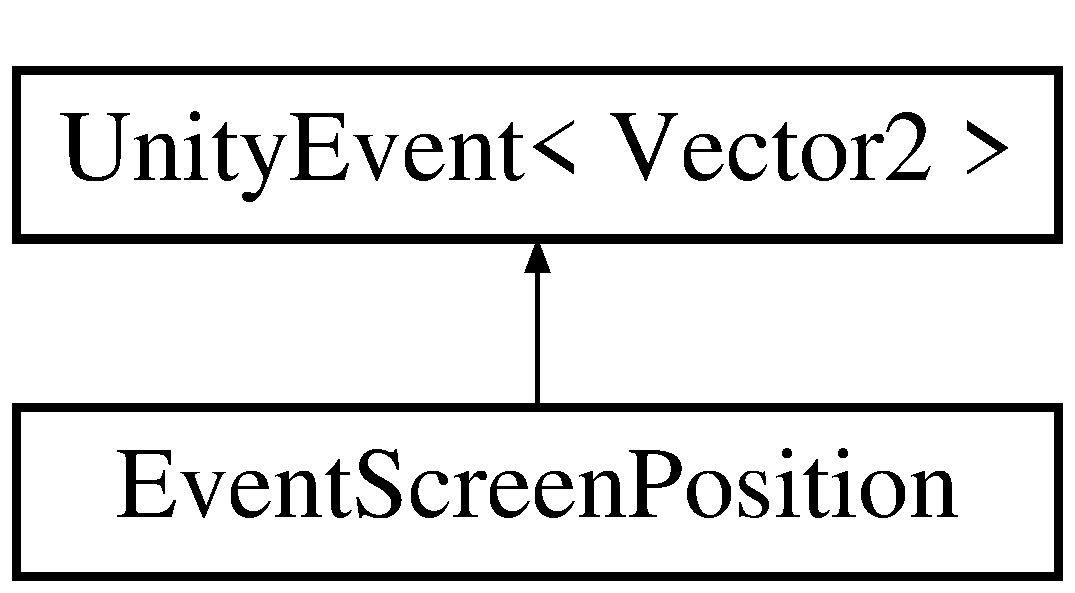
\includegraphics[height=2.000000cm]{class_event_screen_position}
\end{center}
\end{figure}


The documentation for this class was generated from the following file\+:\begin{DoxyCompactItemize}
\item 
Gamejam\+Unity/\+Assets/\+Scripts/Mobile\+Input.\+cs\end{DoxyCompactItemize}

\hypertarget{class_event_string}{}\section{Event\+String Class Reference}
\label{class_event_string}\index{Event\+String@{Event\+String}}
Inheritance diagram for Event\+String\+:\begin{figure}[H]
\begin{center}
\leavevmode
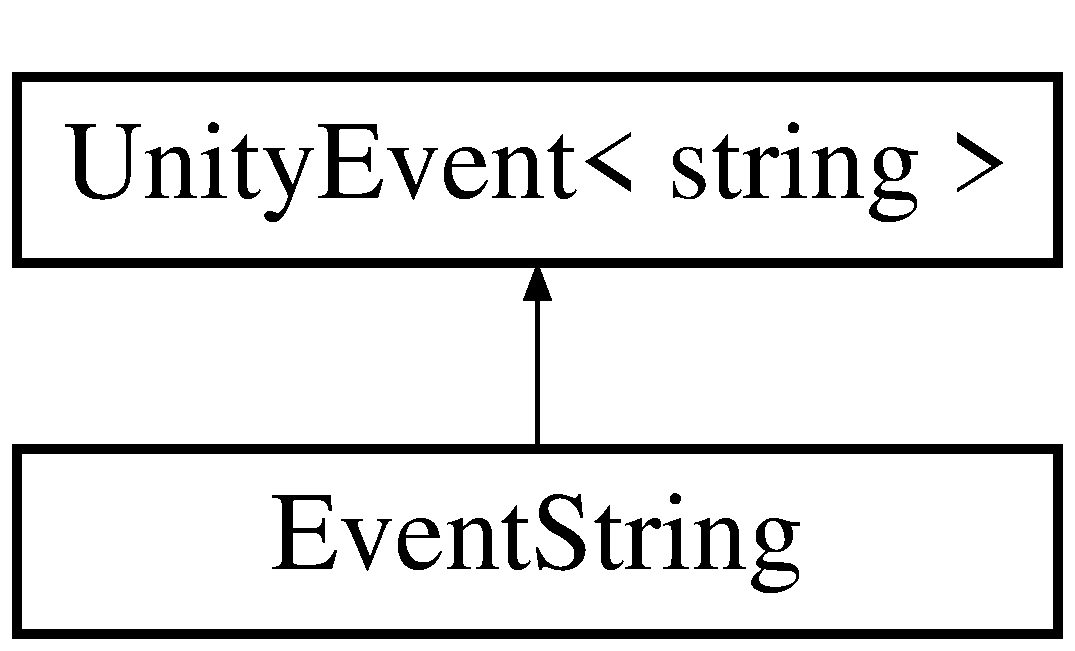
\includegraphics[height=2.000000cm]{class_event_string}
\end{center}
\end{figure}


The documentation for this class was generated from the following file\+:\begin{DoxyCompactItemize}
\item 
Gamejam\+Unity/\+Assets/\+Scripts/Mobile\+Input.\+cs\end{DoxyCompactItemize}

\hypertarget{class_event_test_script}{}\section{Event\+Test\+Script Class Reference}
\label{class_event_test_script}\index{Event\+Test\+Script@{Event\+Test\+Script}}


Just a Testing Script  


Inheritance diagram for Event\+Test\+Script\+:\begin{figure}[H]
\begin{center}
\leavevmode
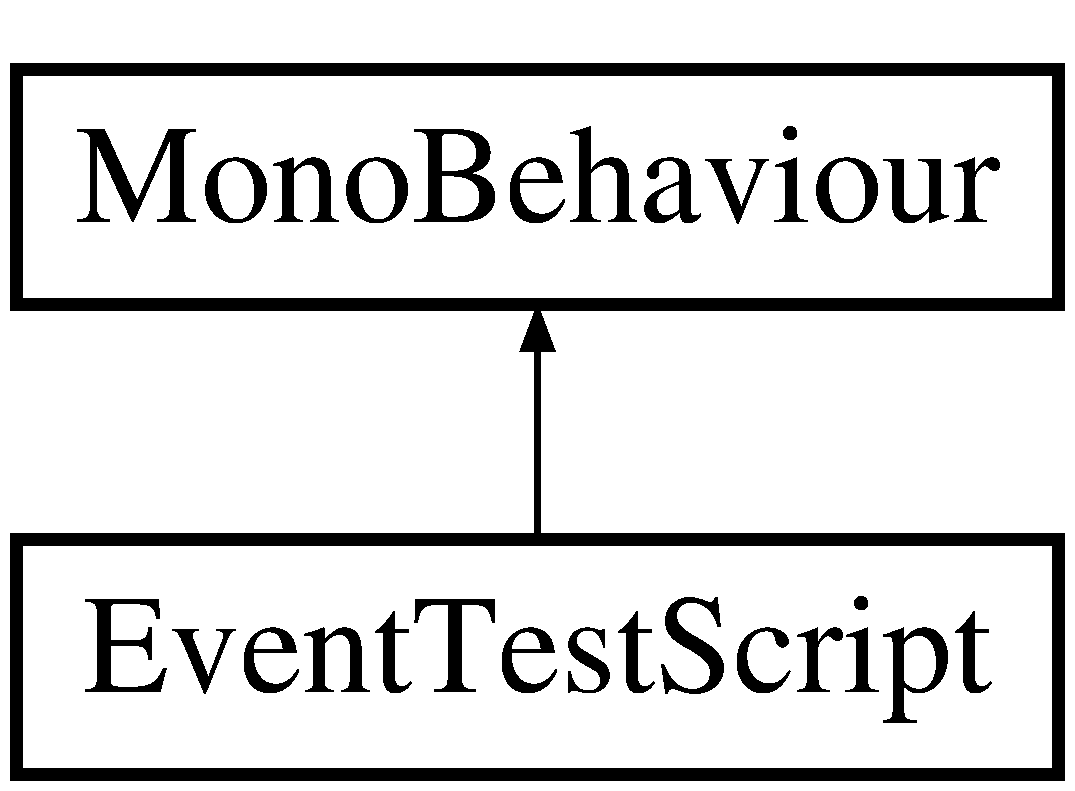
\includegraphics[height=2.000000cm]{class_event_test_script}
\end{center}
\end{figure}


\subsection{Detailed Description}
Just a Testing Script 



The documentation for this class was generated from the following file\+:\begin{DoxyCompactItemize}
\item 
Gamejam\+Unity/\+Assets/\+Scripts/Event\+Test\+Script.\+cs\end{DoxyCompactItemize}

\hypertarget{class_event_threshold_level}{}\section{Event\+Threshold\+Level Class Reference}
\label{class_event_threshold_level}\index{Event\+Threshold\+Level@{Event\+Threshold\+Level}}
Inheritance diagram for Event\+Threshold\+Level\+:\begin{figure}[H]
\begin{center}
\leavevmode
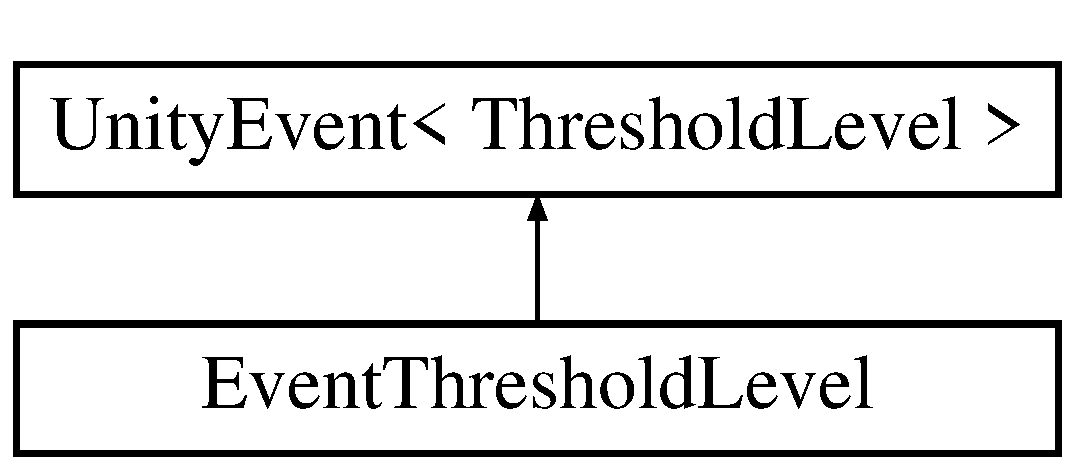
\includegraphics[height=2.000000cm]{class_event_threshold_level}
\end{center}
\end{figure}


The documentation for this class was generated from the following file\+:\begin{DoxyCompactItemize}
\item 
Gamejam\+Unity/\+Assets/\+Scripts/Mobile\+Input.\+cs\end{DoxyCompactItemize}

\hypertarget{class_event_touch}{}\section{Event\+Touch Class Reference}
\label{class_event_touch}\index{Event\+Touch@{Event\+Touch}}
Inheritance diagram for Event\+Touch\+:\begin{figure}[H]
\begin{center}
\leavevmode
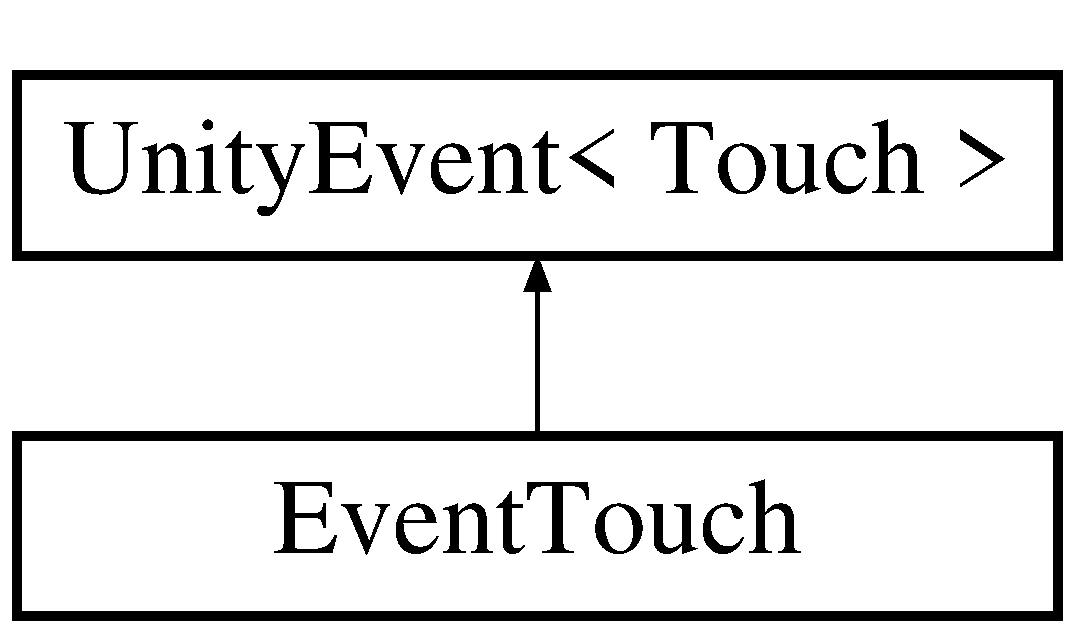
\includegraphics[height=2.000000cm]{class_event_touch}
\end{center}
\end{figure}


The documentation for this class was generated from the following file\+:\begin{DoxyCompactItemize}
\item 
Gamejam\+Unity/\+Assets/\+Scripts/Mobile\+Input.\+cs\end{DoxyCompactItemize}

\hypertarget{class_evil_action}{}\section{Evil\+Action Class Reference}
\label{class_evil_action}\index{Evil\+Action@{Evil\+Action}}
\subsection*{Properties}
\begin{DoxyCompactItemize}
\item 
\mbox{\Hypertarget{class_evil_action_abc6755207782133791be9f3fcbcf3f38}\label{class_evil_action_abc6755207782133791be9f3fcbcf3f38}} 
string {\bfseries Action\+Type}\hspace{0.3cm}{\ttfamily  \mbox{[}get, set\mbox{]}}
\item 
\mbox{\Hypertarget{class_evil_action_aaa3e372427800c55e8a8577f23080103}\label{class_evil_action_aaa3e372427800c55e8a8577f23080103}} 
string {\bfseries Identifier}\hspace{0.3cm}{\ttfamily  \mbox{[}get, set\mbox{]}}
\item 
\mbox{\Hypertarget{class_evil_action_aba365e771fba0af37b9d9dcdf6ce9d85}\label{class_evil_action_aba365e771fba0af37b9d9dcdf6ce9d85}} 
int {\bfseries Peaks}\hspace{0.3cm}{\ttfamily  \mbox{[}get, set\mbox{]}}
\item 
\mbox{\Hypertarget{class_evil_action_ab55a3d31911a5ff2250abc79d34d7d7e}\label{class_evil_action_ab55a3d31911a5ff2250abc79d34d7d7e}} 
int {\bfseries Decibel}\hspace{0.3cm}{\ttfamily  \mbox{[}get, set\mbox{]}}
\item 
\mbox{\Hypertarget{class_evil_action_af03e783992d0a5f35e6a7c677ad1cf38}\label{class_evil_action_af03e783992d0a5f35e6a7c677ad1cf38}} 
string {\bfseries Object\+Of\+Interest}\hspace{0.3cm}{\ttfamily  \mbox{[}get, set\mbox{]}}
\item 
\mbox{\Hypertarget{class_evil_action_ac096415964b737941bc4088a357a79da}\label{class_evil_action_ac096415964b737941bc4088a357a79da}} 
string {\bfseries Placement\+Target}\hspace{0.3cm}{\ttfamily  \mbox{[}get, set\mbox{]}}
\item 
\mbox{\Hypertarget{class_evil_action_a67f145a7e91790942e92ec6e51288499}\label{class_evil_action_a67f145a7e91790942e92ec6e51288499}} 
string {\bfseries details}\hspace{0.3cm}{\ttfamily  \mbox{[}get, set\mbox{]}}
\end{DoxyCompactItemize}


The documentation for this class was generated from the following file\+:\begin{DoxyCompactItemize}
\item 
Gamejam\+Unity/\+Assets/\+Scripts/\+Datastructure/Game\+World.\+cs\end{DoxyCompactItemize}

\hypertarget{class_game_manager}{}\section{Game\+Manager Class Reference}
\label{class_game_manager}\index{Game\+Manager@{Game\+Manager}}
Inheritance diagram for Game\+Manager\+:\begin{figure}[H]
\begin{center}
\leavevmode
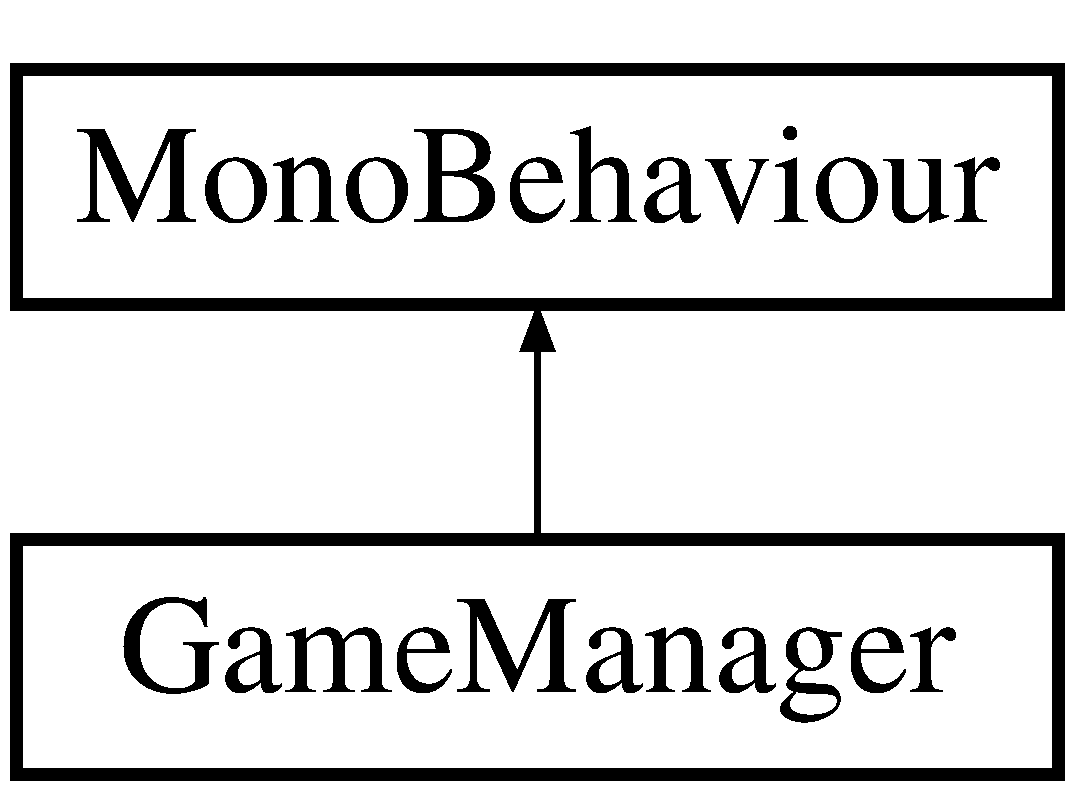
\includegraphics[height=2.000000cm]{class_game_manager}
\end{center}
\end{figure}


The documentation for this class was generated from the following file\+:\begin{DoxyCompactItemize}
\item 
Gamejam\+Unity/\+Assets/\+Scripts/Game\+Manager.\+cs\end{DoxyCompactItemize}

\hypertarget{class_dr_evil_1_1_data_structure_1_1_game_state}{}\section{Dr\+Evil.\+Data\+Structure.\+Game\+State Class Reference}
\label{class_dr_evil_1_1_data_structure_1_1_game_state}\index{Dr\+Evil.\+Data\+Structure.\+Game\+State@{Dr\+Evil.\+Data\+Structure.\+Game\+State}}


This class holds the complete datastructure of the game  


Inheritance diagram for Dr\+Evil.\+Data\+Structure.\+Game\+State\+:\begin{figure}[H]
\begin{center}
\leavevmode
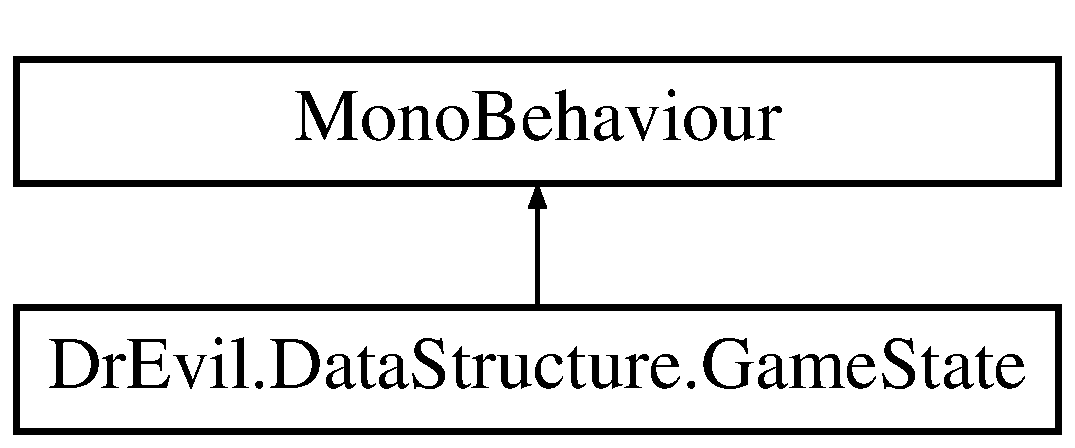
\includegraphics[height=2.000000cm]{class_dr_evil_1_1_data_structure_1_1_game_state}
\end{center}
\end{figure}
\subsection*{Public Member Functions}
\begin{DoxyCompactItemize}
\item 
void \mbox{\hyperlink{class_dr_evil_1_1_data_structure_1_1_game_state_aefeb7ac3d896bc342f85fdd807ab5c82}{Accomplish\+Actual\+Level}} ()
\begin{DoxyCompactList}\small\item\em Finished the Current\+Person and Unlocks the next \mbox{\hyperlink{class_person}{Person}} in the Current\+World \end{DoxyCompactList}\item 
bool \mbox{\hyperlink{class_dr_evil_1_1_data_structure_1_1_game_state_a04198d05c739adf93c35fcfa7aab340a}{Select\+An\+Level}} (\mbox{\hyperlink{class_person}{Person}} new\+Person)
\begin{DoxyCompactList}\small\item\em Select a level depending on a person \end{DoxyCompactList}\item 
void \mbox{\hyperlink{class_dr_evil_1_1_data_structure_1_1_game_state_ac34f35978eeba7de0ba96b018b8216c4}{Reset\+Level}} (\mbox{\hyperlink{class_person}{Person}} person)
\begin{DoxyCompactList}\small\item\em Reset a level depending on person \end{DoxyCompactList}\item 
bool \mbox{\hyperlink{class_dr_evil_1_1_data_structure_1_1_game_state_a5d26d915d3a81df99b17402e49491a80}{Solve\+Action}} (\mbox{\hyperlink{class_evil_action}{Evil\+Action}} action)
\begin{DoxyCompactList}\small\item\em Solve an action for the current level \end{DoxyCompactList}\end{DoxyCompactItemize}
\subsection*{Public Attributes}
\begin{DoxyCompactItemize}
\item 
\mbox{\Hypertarget{class_dr_evil_1_1_data_structure_1_1_game_state_a3cd50bc1107cf91ccbec13fd363aa2be}\label{class_dr_evil_1_1_data_structure_1_1_game_state_a3cd50bc1107cf91ccbec13fd363aa2be}} 
Text\+Asset {\bfseries Input\+File\+Text\+Asset}
\item 
\mbox{\Hypertarget{class_dr_evil_1_1_data_structure_1_1_game_state_a0d6c7d61daeaf90c98e2b209afe31a32}\label{class_dr_evil_1_1_data_structure_1_1_game_state_a0d6c7d61daeaf90c98e2b209afe31a32}} 
\mbox{\hyperlink{class_world}{World}} {\bfseries raw\+Data}
\item 
\mbox{\Hypertarget{class_dr_evil_1_1_data_structure_1_1_game_state_a848ec94c9cd5ba5bd30436c0c4d3b52c}\label{class_dr_evil_1_1_data_structure_1_1_game_state_a848ec94c9cd5ba5bd30436c0c4d3b52c}} 
\mbox{\hyperlink{class_world}{World}} {\bfseries Current\+World}
\item 
\mbox{\Hypertarget{class_dr_evil_1_1_data_structure_1_1_game_state_a64868955af5972ecc885155f450c368a}\label{class_dr_evil_1_1_data_structure_1_1_game_state_a64868955af5972ecc885155f450c368a}} 
\mbox{\hyperlink{class_person}{Person}} {\bfseries Current\+Person}
\end{DoxyCompactItemize}
\subsection*{Static Public Attributes}
\begin{DoxyCompactItemize}
\item 
\mbox{\Hypertarget{class_dr_evil_1_1_data_structure_1_1_game_state_a84e4952e23177b41b6c94c25add295af}\label{class_dr_evil_1_1_data_structure_1_1_game_state_a84e4952e23177b41b6c94c25add295af}} 
static \mbox{\hyperlink{class_dr_evil_1_1_data_structure_1_1_game_state}{Game\+State}} {\bfseries instance}
\end{DoxyCompactItemize}


\subsection{Detailed Description}
This class holds the complete datastructure of the game 



\subsection{Member Function Documentation}
\mbox{\Hypertarget{class_dr_evil_1_1_data_structure_1_1_game_state_aefeb7ac3d896bc342f85fdd807ab5c82}\label{class_dr_evil_1_1_data_structure_1_1_game_state_aefeb7ac3d896bc342f85fdd807ab5c82}} 
\index{Dr\+Evil\+::\+Data\+Structure\+::\+Game\+State@{Dr\+Evil\+::\+Data\+Structure\+::\+Game\+State}!Accomplish\+Actual\+Level@{Accomplish\+Actual\+Level}}
\index{Accomplish\+Actual\+Level@{Accomplish\+Actual\+Level}!Dr\+Evil\+::\+Data\+Structure\+::\+Game\+State@{Dr\+Evil\+::\+Data\+Structure\+::\+Game\+State}}
\subsubsection{\texorpdfstring{Accomplish\+Actual\+Level()}{AccomplishActualLevel()}}
{\footnotesize\ttfamily void Dr\+Evil.\+Data\+Structure.\+Game\+State.\+Accomplish\+Actual\+Level (\begin{DoxyParamCaption}{ }\end{DoxyParamCaption})\hspace{0.3cm}{\ttfamily [inline]}}



Finished the Current\+Person and Unlocks the next \mbox{\hyperlink{class_person}{Person}} in the Current\+World 

\mbox{\Hypertarget{class_dr_evil_1_1_data_structure_1_1_game_state_ac34f35978eeba7de0ba96b018b8216c4}\label{class_dr_evil_1_1_data_structure_1_1_game_state_ac34f35978eeba7de0ba96b018b8216c4}} 
\index{Dr\+Evil\+::\+Data\+Structure\+::\+Game\+State@{Dr\+Evil\+::\+Data\+Structure\+::\+Game\+State}!Reset\+Level@{Reset\+Level}}
\index{Reset\+Level@{Reset\+Level}!Dr\+Evil\+::\+Data\+Structure\+::\+Game\+State@{Dr\+Evil\+::\+Data\+Structure\+::\+Game\+State}}
\subsubsection{\texorpdfstring{Reset\+Level()}{ResetLevel()}}
{\footnotesize\ttfamily void Dr\+Evil.\+Data\+Structure.\+Game\+State.\+Reset\+Level (\begin{DoxyParamCaption}\item[{\mbox{\hyperlink{class_person}{Person}}}]{person }\end{DoxyParamCaption})\hspace{0.3cm}{\ttfamily [inline]}}



Reset a level depending on person 


\begin{DoxyParams}{Parameters}
{\em person} & \\
\hline
\end{DoxyParams}
\mbox{\Hypertarget{class_dr_evil_1_1_data_structure_1_1_game_state_a04198d05c739adf93c35fcfa7aab340a}\label{class_dr_evil_1_1_data_structure_1_1_game_state_a04198d05c739adf93c35fcfa7aab340a}} 
\index{Dr\+Evil\+::\+Data\+Structure\+::\+Game\+State@{Dr\+Evil\+::\+Data\+Structure\+::\+Game\+State}!Select\+An\+Level@{Select\+An\+Level}}
\index{Select\+An\+Level@{Select\+An\+Level}!Dr\+Evil\+::\+Data\+Structure\+::\+Game\+State@{Dr\+Evil\+::\+Data\+Structure\+::\+Game\+State}}
\subsubsection{\texorpdfstring{Select\+An\+Level()}{SelectAnLevel()}}
{\footnotesize\ttfamily bool Dr\+Evil.\+Data\+Structure.\+Game\+State.\+Select\+An\+Level (\begin{DoxyParamCaption}\item[{\mbox{\hyperlink{class_person}{Person}}}]{new\+Person }\end{DoxyParamCaption})\hspace{0.3cm}{\ttfamily [inline]}}



Select a level depending on a person 


\begin{DoxyParams}{Parameters}
{\em new\+Person} & \\
\hline
\end{DoxyParams}
\begin{DoxyReturn}{Returns}

\end{DoxyReturn}
\mbox{\Hypertarget{class_dr_evil_1_1_data_structure_1_1_game_state_a5d26d915d3a81df99b17402e49491a80}\label{class_dr_evil_1_1_data_structure_1_1_game_state_a5d26d915d3a81df99b17402e49491a80}} 
\index{Dr\+Evil\+::\+Data\+Structure\+::\+Game\+State@{Dr\+Evil\+::\+Data\+Structure\+::\+Game\+State}!Solve\+Action@{Solve\+Action}}
\index{Solve\+Action@{Solve\+Action}!Dr\+Evil\+::\+Data\+Structure\+::\+Game\+State@{Dr\+Evil\+::\+Data\+Structure\+::\+Game\+State}}
\subsubsection{\texorpdfstring{Solve\+Action()}{SolveAction()}}
{\footnotesize\ttfamily bool Dr\+Evil.\+Data\+Structure.\+Game\+State.\+Solve\+Action (\begin{DoxyParamCaption}\item[{\mbox{\hyperlink{class_evil_action}{Evil\+Action}}}]{action }\end{DoxyParamCaption})\hspace{0.3cm}{\ttfamily [inline]}}



Solve an action for the current level 


\begin{DoxyParams}{Parameters}
{\em action} & \\
\hline
\end{DoxyParams}
\begin{DoxyReturn}{Returns}

\end{DoxyReturn}


The documentation for this class was generated from the following file\+:\begin{DoxyCompactItemize}
\item 
Gamejam\+Unity/\+Assets/\+Scripts/Game\+State.\+cs\end{DoxyCompactItemize}

\hypertarget{class_mobile_sensors_1_1_gyro_camera}{}\section{Mobile\+Sensors.\+Gyro\+Camera Class Reference}
\label{class_mobile_sensors_1_1_gyro_camera}\index{Mobile\+Sensors.\+Gyro\+Camera@{Mobile\+Sensors.\+Gyro\+Camera}}


Applying the gyro input to the gyro camera  


Inheritance diagram for Mobile\+Sensors.\+Gyro\+Camera\+:\begin{figure}[H]
\begin{center}
\leavevmode
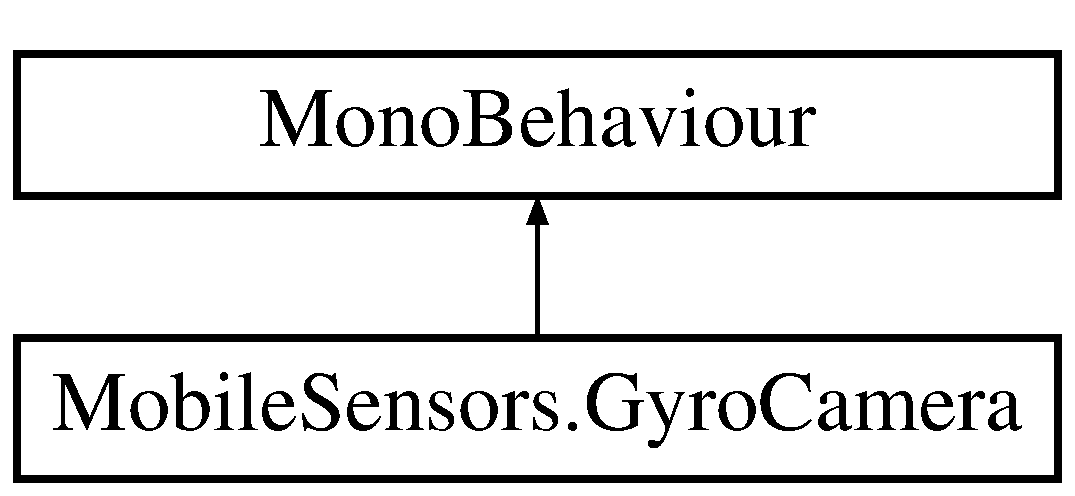
\includegraphics[height=2.000000cm]{class_mobile_sensors_1_1_gyro_camera}
\end{center}
\end{figure}


\subsection{Detailed Description}
Applying the gyro input to the gyro camera 



The documentation for this class was generated from the following file\+:\begin{DoxyCompactItemize}
\item 
Gamejam\+Unity/\+Assets/\+Scripts/Gyro\+Camera.\+cs\end{DoxyCompactItemize}

\hypertarget{class_dr_evil_1_1_visuals_1_1_highightable_object}{}\section{Dr\+Evil.\+Visuals.\+Highightable\+Object Class Reference}
\label{class_dr_evil_1_1_visuals_1_1_highightable_object}\index{Dr\+Evil.\+Visuals.\+Highightable\+Object@{Dr\+Evil.\+Visuals.\+Highightable\+Object}}


Simple class to highlight aimed objects  


Inheritance diagram for Dr\+Evil.\+Visuals.\+Highightable\+Object\+:\begin{figure}[H]
\begin{center}
\leavevmode
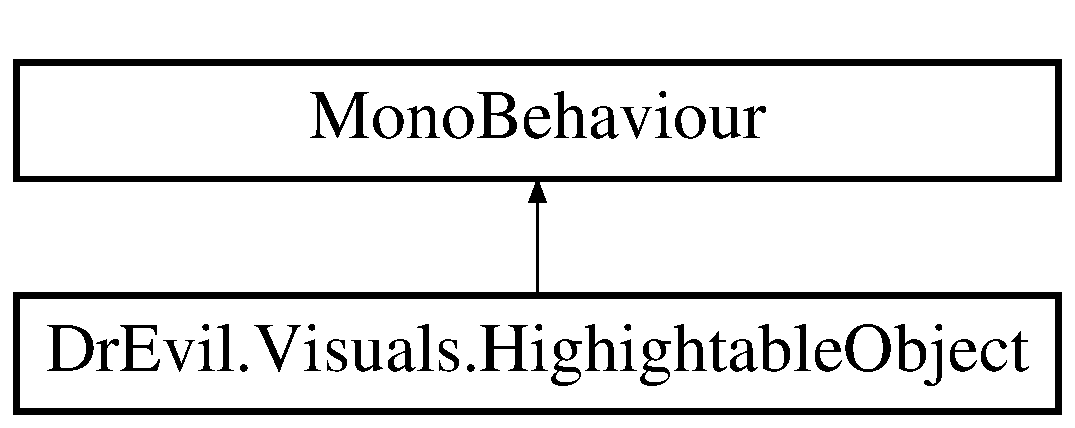
\includegraphics[height=2.000000cm]{class_dr_evil_1_1_visuals_1_1_highightable_object}
\end{center}
\end{figure}
\subsection*{Public Member Functions}
\begin{DoxyCompactItemize}
\item 
void \mbox{\hyperlink{class_dr_evil_1_1_visuals_1_1_highightable_object_aaade7ada66cdac85e38045579c4cb447}{Enable\+Highlight}} ()
\begin{DoxyCompactList}\small\item\em Highlight object \end{DoxyCompactList}\item 
void \mbox{\hyperlink{class_dr_evil_1_1_visuals_1_1_highightable_object_a6b59e8e3ac556d65eb93a304be07c18f}{Disable\+Highlight}} ()
\begin{DoxyCompactList}\small\item\em Dehighlight object \end{DoxyCompactList}\end{DoxyCompactItemize}
\subsection*{Public Attributes}
\begin{DoxyCompactItemize}
\item 
\mbox{\Hypertarget{class_dr_evil_1_1_visuals_1_1_highightable_object_a42d4de1f0af915d44f04d00319be2388}\label{class_dr_evil_1_1_visuals_1_1_highightable_object_a42d4de1f0af915d44f04d00319be2388}} 
float {\bfseries Out\+Line\+Min} = 0.\+0f
\item 
\mbox{\Hypertarget{class_dr_evil_1_1_visuals_1_1_highightable_object_ab91f29ea399951a14f924b079e3e7a4b}\label{class_dr_evil_1_1_visuals_1_1_highightable_object_ab91f29ea399951a14f924b079e3e7a4b}} 
float {\bfseries Outline\+Max} = 0.\+05f
\item 
\mbox{\Hypertarget{class_dr_evil_1_1_visuals_1_1_highightable_object_ac0cd769e08f6d91f9ad2f880d2ac1943}\label{class_dr_evil_1_1_visuals_1_1_highightable_object_ac0cd769e08f6d91f9ad2f880d2ac1943}} 
Material {\bfseries Outline\+Material}
\end{DoxyCompactItemize}


\subsection{Detailed Description}
Simple class to highlight aimed objects 



\subsection{Member Function Documentation}
\mbox{\Hypertarget{class_dr_evil_1_1_visuals_1_1_highightable_object_a6b59e8e3ac556d65eb93a304be07c18f}\label{class_dr_evil_1_1_visuals_1_1_highightable_object_a6b59e8e3ac556d65eb93a304be07c18f}} 
\index{Dr\+Evil\+::\+Visuals\+::\+Highightable\+Object@{Dr\+Evil\+::\+Visuals\+::\+Highightable\+Object}!Disable\+Highlight@{Disable\+Highlight}}
\index{Disable\+Highlight@{Disable\+Highlight}!Dr\+Evil\+::\+Visuals\+::\+Highightable\+Object@{Dr\+Evil\+::\+Visuals\+::\+Highightable\+Object}}
\subsubsection{\texorpdfstring{Disable\+Highlight()}{DisableHighlight()}}
{\footnotesize\ttfamily void Dr\+Evil.\+Visuals.\+Highightable\+Object.\+Disable\+Highlight (\begin{DoxyParamCaption}{ }\end{DoxyParamCaption})\hspace{0.3cm}{\ttfamily [inline]}}



Dehighlight object 

\mbox{\Hypertarget{class_dr_evil_1_1_visuals_1_1_highightable_object_aaade7ada66cdac85e38045579c4cb447}\label{class_dr_evil_1_1_visuals_1_1_highightable_object_aaade7ada66cdac85e38045579c4cb447}} 
\index{Dr\+Evil\+::\+Visuals\+::\+Highightable\+Object@{Dr\+Evil\+::\+Visuals\+::\+Highightable\+Object}!Enable\+Highlight@{Enable\+Highlight}}
\index{Enable\+Highlight@{Enable\+Highlight}!Dr\+Evil\+::\+Visuals\+::\+Highightable\+Object@{Dr\+Evil\+::\+Visuals\+::\+Highightable\+Object}}
\subsubsection{\texorpdfstring{Enable\+Highlight()}{EnableHighlight()}}
{\footnotesize\ttfamily void Dr\+Evil.\+Visuals.\+Highightable\+Object.\+Enable\+Highlight (\begin{DoxyParamCaption}{ }\end{DoxyParamCaption})\hspace{0.3cm}{\ttfamily [inline]}}



Highlight object 



The documentation for this class was generated from the following file\+:\begin{DoxyCompactItemize}
\item 
Gamejam\+Unity/\+Assets/\+Scripts/Highightable\+Object.\+cs\end{DoxyCompactItemize}

\hypertarget{class_dr_evil_1_1_visuals_1_1_interactable_object_hghlighter}{}\section{Dr\+Evil.\+Visuals.\+Interactable\+Object\+Hghlighter Class Reference}
\label{class_dr_evil_1_1_visuals_1_1_interactable_object_hghlighter}\index{Dr\+Evil.\+Visuals.\+Interactable\+Object\+Hghlighter@{Dr\+Evil.\+Visuals.\+Interactable\+Object\+Hghlighter}}


Class for highlighting and updating interactable objects  


Inheritance diagram for Dr\+Evil.\+Visuals.\+Interactable\+Object\+Hghlighter\+:\begin{figure}[H]
\begin{center}
\leavevmode
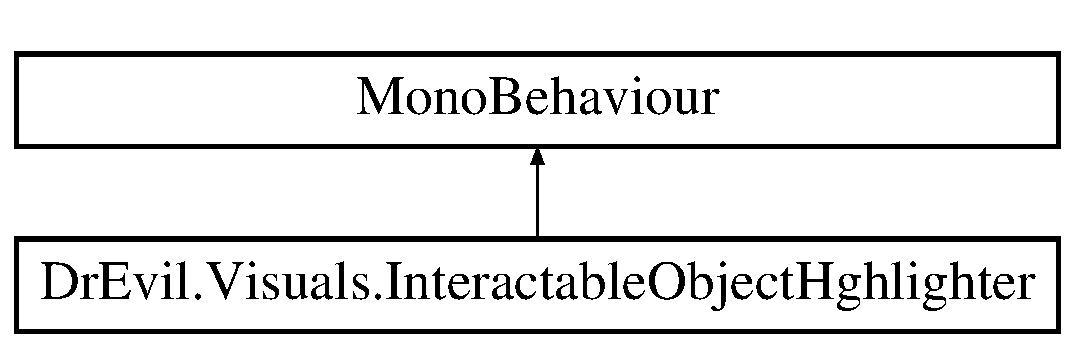
\includegraphics[height=2.000000cm]{class_dr_evil_1_1_visuals_1_1_interactable_object_hghlighter}
\end{center}
\end{figure}
\subsection*{Public Attributes}
\begin{DoxyCompactItemize}
\item 
\mbox{\Hypertarget{class_dr_evil_1_1_visuals_1_1_interactable_object_hghlighter_a2231ad7c16ddcaea6f61cd42f75ce402}\label{class_dr_evil_1_1_visuals_1_1_interactable_object_hghlighter_a2231ad7c16ddcaea6f61cd42f75ce402}} 
Camera {\bfseries Gyro\+Cam}
\end{DoxyCompactItemize}


\subsection{Detailed Description}
Class for highlighting and updating interactable objects 



The documentation for this class was generated from the following file\+:\begin{DoxyCompactItemize}
\item 
Gamejam\+Unity/\+Assets/\+Scripts/Interactable\+Object\+Hghlighter.\+cs\end{DoxyCompactItemize}

\hypertarget{interface_interaction_trigger}{}\section{Interaction\+Trigger Interface Reference}
\label{interface_interaction_trigger}\index{Interaction\+Trigger@{Interaction\+Trigger}}
Inheritance diagram for Interaction\+Trigger\+:\begin{figure}[H]
\begin{center}
\leavevmode
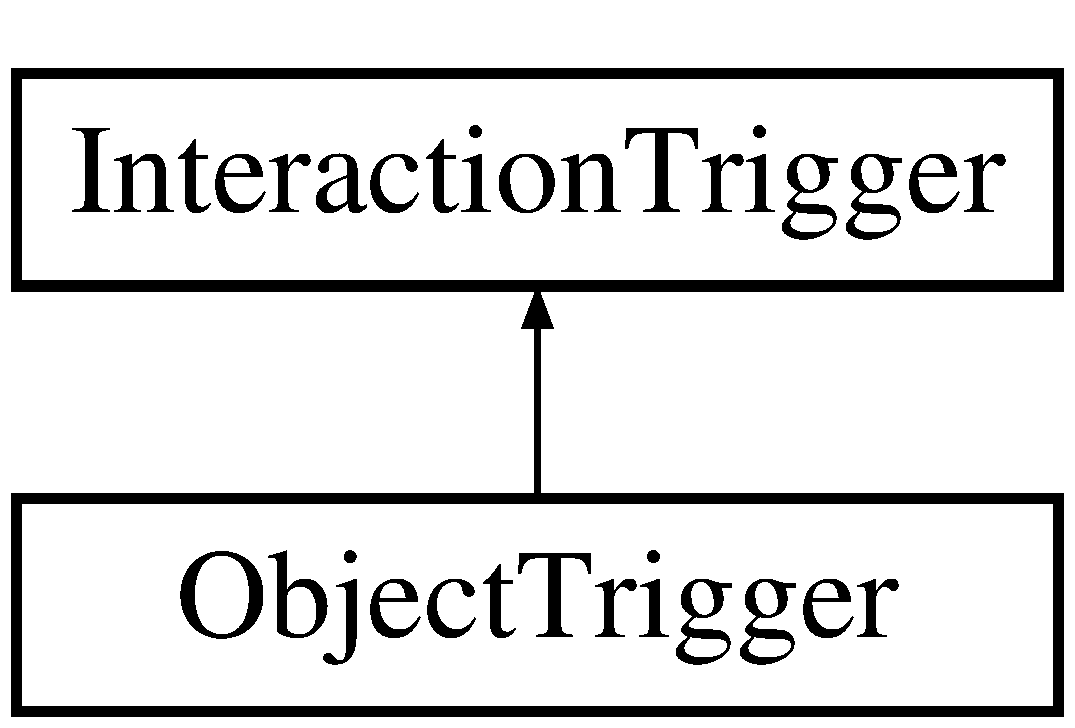
\includegraphics[height=2.000000cm]{interface_interaction_trigger}
\end{center}
\end{figure}
\subsection*{Public Member Functions}
\begin{DoxyCompactItemize}
\item 
\mbox{\Hypertarget{interface_interaction_trigger_a0a5bff66e684f928a92c042fadbea146}\label{interface_interaction_trigger_a0a5bff66e684f928a92c042fadbea146}} 
I\+Enumerator {\bfseries Trigger\+Action} (Action\+Complete action)
\item 
\mbox{\Hypertarget{interface_interaction_trigger_adcef766c061402978863e72d622d1998}\label{interface_interaction_trigger_adcef766c061402978863e72d622d1998}} 
void {\bfseries Stop\+Action} ()
\item 
\mbox{\Hypertarget{interface_interaction_trigger_a60432c03fbcad7c76a9078acaec32fe1}\label{interface_interaction_trigger_a60432c03fbcad7c76a9078acaec32fe1}} 
void {\bfseries Action\+Completed} ()
\end{DoxyCompactItemize}


The documentation for this interface was generated from the following file\+:\begin{DoxyCompactItemize}
\item 
Gamejam\+Unity/\+Assets/\+Scripts/Terror\+Level\+Controller.\+cs\end{DoxyCompactItemize}

\hypertarget{class_dr_evil_1_1_testing_1_1_level_accomplish_test}{}\section{Dr\+Evil.\+Testing.\+Level\+Accomplish\+Test Class Reference}
\label{class_dr_evil_1_1_testing_1_1_level_accomplish_test}\index{Dr\+Evil.\+Testing.\+Level\+Accomplish\+Test@{Dr\+Evil.\+Testing.\+Level\+Accomplish\+Test}}
Inheritance diagram for Dr\+Evil.\+Testing.\+Level\+Accomplish\+Test\+:\begin{figure}[H]
\begin{center}
\leavevmode
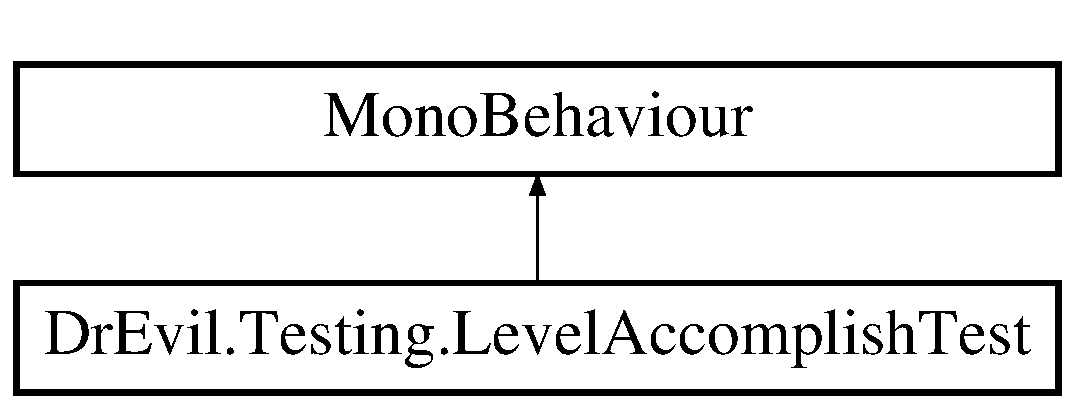
\includegraphics[height=2.000000cm]{class_dr_evil_1_1_testing_1_1_level_accomplish_test}
\end{center}
\end{figure}
\subsection*{Public Attributes}
\begin{DoxyCompactItemize}
\item 
\mbox{\Hypertarget{class_dr_evil_1_1_testing_1_1_level_accomplish_test_a7429628baae1d4e1efa47e55ec9d10f8}\label{class_dr_evil_1_1_testing_1_1_level_accomplish_test_a7429628baae1d4e1efa47e55ec9d10f8}} 
Button {\bfseries test}
\item 
\mbox{\Hypertarget{class_dr_evil_1_1_testing_1_1_level_accomplish_test_ad5896dde647d015c93eb117a94e2b361}\label{class_dr_evil_1_1_testing_1_1_level_accomplish_test_ad5896dde647d015c93eb117a94e2b361}} 
Unity\+Event$<$ bool $>$ {\bfseries on\+Level\+Is\+Over}
\end{DoxyCompactItemize}
\subsection*{Static Public Attributes}
\begin{DoxyCompactItemize}
\item 
\mbox{\Hypertarget{class_dr_evil_1_1_testing_1_1_level_accomplish_test_a3d4e82176ff41b160213f464fc55df6e}\label{class_dr_evil_1_1_testing_1_1_level_accomplish_test_a3d4e82176ff41b160213f464fc55df6e}} 
static \mbox{\hyperlink{class_dr_evil_1_1_testing_1_1_level_accomplish_test}{Level\+Accomplish\+Test}} {\bfseries instance}
\end{DoxyCompactItemize}


The documentation for this class was generated from the following file\+:\begin{DoxyCompactItemize}
\item 
Gamejam\+Unity/\+Assets/Level\+Accomplish\+Test.\+cs\end{DoxyCompactItemize}

\hypertarget{class_dr_evil_1_1_testing_1_1_level_is_over}{}\section{Dr\+Evil.\+Testing.\+Level\+Is\+Over Class Reference}
\label{class_dr_evil_1_1_testing_1_1_level_is_over}\index{Dr\+Evil.\+Testing.\+Level\+Is\+Over@{Dr\+Evil.\+Testing.\+Level\+Is\+Over}}
Inheritance diagram for Dr\+Evil.\+Testing.\+Level\+Is\+Over\+:\begin{figure}[H]
\begin{center}
\leavevmode
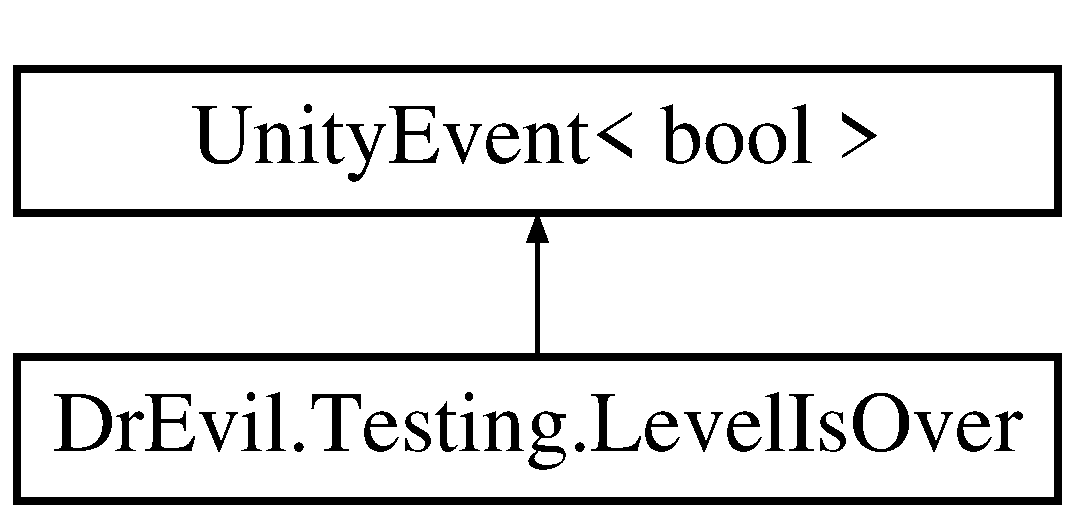
\includegraphics[height=2.000000cm]{class_dr_evil_1_1_testing_1_1_level_is_over}
\end{center}
\end{figure}


The documentation for this class was generated from the following file\+:\begin{DoxyCompactItemize}
\item 
Gamejam\+Unity/\+Assets/Level\+Accomplish\+Test.\+cs\end{DoxyCompactItemize}

\hypertarget{class_dr_evil_1_1_mechanics_1_1_map_view_controller}{}\section{Dr\+Evil.\+Mechanics.\+Map\+View\+Controller Class Reference}
\label{class_dr_evil_1_1_mechanics_1_1_map_view_controller}\index{Dr\+Evil.\+Mechanics.\+Map\+View\+Controller@{Dr\+Evil.\+Mechanics.\+Map\+View\+Controller}}
Inheritance diagram for Dr\+Evil.\+Mechanics.\+Map\+View\+Controller\+:\begin{figure}[H]
\begin{center}
\leavevmode
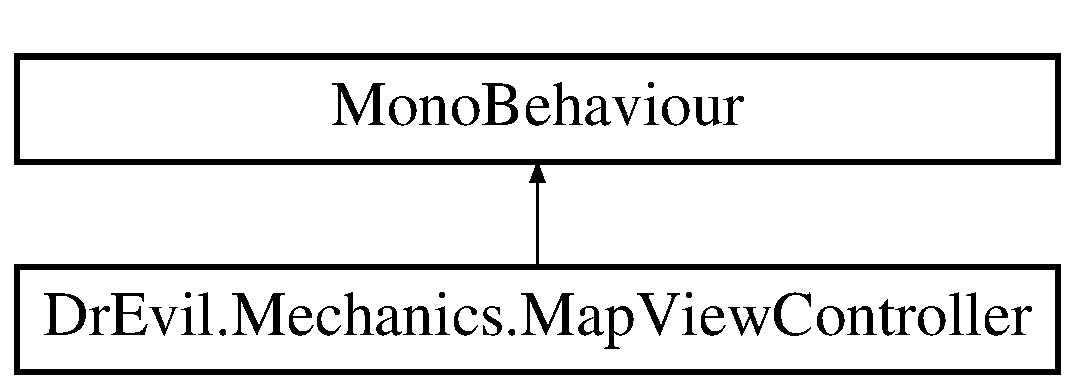
\includegraphics[height=2.000000cm]{class_dr_evil_1_1_mechanics_1_1_map_view_controller}
\end{center}
\end{figure}
\subsection*{Public Member Functions}
\begin{DoxyCompactItemize}
\item 
void \mbox{\hyperlink{class_dr_evil_1_1_mechanics_1_1_map_view_controller_a1a62e396bd481e7d1b88accd03fc32f5}{Enter\+Mini\+Map}} ()
\begin{DoxyCompactList}\small\item\em Call this whenever the minimap is entered to refresh level button states \end{DoxyCompactList}\end{DoxyCompactItemize}
\subsection*{Public Attributes}
\begin{DoxyCompactItemize}
\item 
\mbox{\Hypertarget{class_dr_evil_1_1_mechanics_1_1_map_view_controller_ada098364404f391bea28629efe7d78c7}\label{class_dr_evil_1_1_mechanics_1_1_map_view_controller_ada098364404f391bea28629efe7d78c7}} 
Button {\bfseries Level1\+Button}
\item 
\mbox{\Hypertarget{class_dr_evil_1_1_mechanics_1_1_map_view_controller_acb25ba3785fdfc713dcb662ee9092237}\label{class_dr_evil_1_1_mechanics_1_1_map_view_controller_acb25ba3785fdfc713dcb662ee9092237}} 
Button {\bfseries Level2\+Button}
\item 
\mbox{\Hypertarget{class_dr_evil_1_1_mechanics_1_1_map_view_controller_a24e8df8184088fddba5cecb370179c1f}\label{class_dr_evil_1_1_mechanics_1_1_map_view_controller_a24e8df8184088fddba5cecb370179c1f}} 
Button {\bfseries Level3\+Button}
\item 
\mbox{\Hypertarget{class_dr_evil_1_1_mechanics_1_1_map_view_controller_aef72297ae6e4f87c4a72379016cba569}\label{class_dr_evil_1_1_mechanics_1_1_map_view_controller_aef72297ae6e4f87c4a72379016cba569}} 
Button {\bfseries Level4\+Button}
\item 
\mbox{\Hypertarget{class_dr_evil_1_1_mechanics_1_1_map_view_controller_a06215d41d95c702d58ee1e8fcd176c7c}\label{class_dr_evil_1_1_mechanics_1_1_map_view_controller_a06215d41d95c702d58ee1e8fcd176c7c}} 
Sprite {\bfseries Level\+\_\+1\+Sprite\+\_\+\+In\+Active}
\item 
\mbox{\Hypertarget{class_dr_evil_1_1_mechanics_1_1_map_view_controller_aad917f9cb24d2a92b101d830e521d46a}\label{class_dr_evil_1_1_mechanics_1_1_map_view_controller_aad917f9cb24d2a92b101d830e521d46a}} 
Sprite {\bfseries Level\+\_\+2\+Sprite\+\_\+\+In\+Active}
\item 
\mbox{\Hypertarget{class_dr_evil_1_1_mechanics_1_1_map_view_controller_acf6e487ccdeb97df70b1c8870aa45cfa}\label{class_dr_evil_1_1_mechanics_1_1_map_view_controller_acf6e487ccdeb97df70b1c8870aa45cfa}} 
Sprite {\bfseries Level\+\_\+3\+Sprite\+\_\+\+In\+Active}
\item 
\mbox{\Hypertarget{class_dr_evil_1_1_mechanics_1_1_map_view_controller_ad7e9e6404ee3817bd0157bb7f707d558}\label{class_dr_evil_1_1_mechanics_1_1_map_view_controller_ad7e9e6404ee3817bd0157bb7f707d558}} 
Sprite {\bfseries Level\+\_\+4\+Sprite\+\_\+\+In\+Active}
\end{DoxyCompactItemize}


\subsection{Member Function Documentation}
\mbox{\Hypertarget{class_dr_evil_1_1_mechanics_1_1_map_view_controller_a1a62e396bd481e7d1b88accd03fc32f5}\label{class_dr_evil_1_1_mechanics_1_1_map_view_controller_a1a62e396bd481e7d1b88accd03fc32f5}} 
\index{Dr\+Evil\+::\+Mechanics\+::\+Map\+View\+Controller@{Dr\+Evil\+::\+Mechanics\+::\+Map\+View\+Controller}!Enter\+Mini\+Map@{Enter\+Mini\+Map}}
\index{Enter\+Mini\+Map@{Enter\+Mini\+Map}!Dr\+Evil\+::\+Mechanics\+::\+Map\+View\+Controller@{Dr\+Evil\+::\+Mechanics\+::\+Map\+View\+Controller}}
\subsubsection{\texorpdfstring{Enter\+Mini\+Map()}{EnterMiniMap()}}
{\footnotesize\ttfamily void Dr\+Evil.\+Mechanics.\+Map\+View\+Controller.\+Enter\+Mini\+Map (\begin{DoxyParamCaption}{ }\end{DoxyParamCaption})\hspace{0.3cm}{\ttfamily [inline]}}



Call this whenever the minimap is entered to refresh level button states 



The documentation for this class was generated from the following file\+:\begin{DoxyCompactItemize}
\item 
Gamejam\+Unity/\+Assets/\+Scripts/Map\+View\+Controller.\+cs\end{DoxyCompactItemize}

\hypertarget{class_mobile_sensors_1_1_mobile_input}{}\section{Mobile\+Sensors.\+Mobile\+Input Class Reference}
\label{class_mobile_sensors_1_1_mobile_input}\index{Mobile\+Sensors.\+Mobile\+Input@{Mobile\+Sensors.\+Mobile\+Input}}


This class handles A\+LL mobile inputs. This class can be accessed from everywhere  


Inheritance diagram for Mobile\+Sensors.\+Mobile\+Input\+:\begin{figure}[H]
\begin{center}
\leavevmode
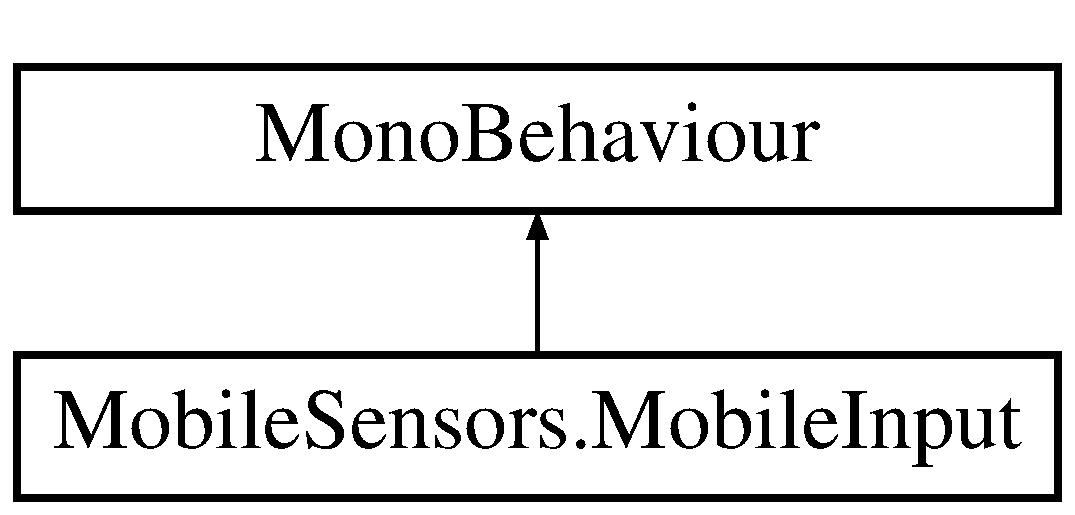
\includegraphics[height=2.000000cm]{class_mobile_sensors_1_1_mobile_input}
\end{center}
\end{figure}
\subsection*{Public Member Functions}
\begin{DoxyCompactItemize}
\item 
Game\+Object \mbox{\hyperlink{class_mobile_sensors_1_1_mobile_input_a65f291342aee293cd5df1684318e4440}{Cast\+Ray\+Hit\+From\+Cam}} (Vector2 pos, Camera cam, int layer\+Mask=8)
\begin{DoxyCompactList}\small\item\em Helper method to raycast and hit from a cam to a layer \end{DoxyCompactList}\end{DoxyCompactItemize}
\subsection*{Public Attributes}
\begin{DoxyCompactItemize}
\item 
\mbox{\Hypertarget{class_mobile_sensors_1_1_mobile_input_ababe459fb35f3fbefa78a6cbe77aacb0}\label{class_mobile_sensors_1_1_mobile_input_ababe459fb35f3fbefa78a6cbe77aacb0}} 
Touch\+Input {\bfseries touch}
\item 
\mbox{\Hypertarget{class_mobile_sensors_1_1_mobile_input_ad2f6ad5bca1a294c41b2404300e83d04}\label{class_mobile_sensors_1_1_mobile_input_ad2f6ad5bca1a294c41b2404300e83d04}} 
Mic {\bfseries mic}
\item 
\mbox{\Hypertarget{class_mobile_sensors_1_1_mobile_input_a2e73a5efc826fecac5fd3b7e518d0876}\label{class_mobile_sensors_1_1_mobile_input_a2e73a5efc826fecac5fd3b7e518d0876}} 
Accelerate {\bfseries accel}
\item 
\mbox{\Hypertarget{class_mobile_sensors_1_1_mobile_input_a3b60d423749d52469e54b5cd6b9cc16c}\label{class_mobile_sensors_1_1_mobile_input_a3b60d423749d52469e54b5cd6b9cc16c}} 
Gyro {\bfseries gyro}
\item 
\mbox{\Hypertarget{class_mobile_sensors_1_1_mobile_input_a7a33d7de90cede62e15e0b0805590139}\label{class_mobile_sensors_1_1_mobile_input_a7a33d7de90cede62e15e0b0805590139}} 
Unity\+Event {\bfseries On\+Unity\+Remote\+Started}
\end{DoxyCompactItemize}
\subsection*{Static Public Attributes}
\begin{DoxyCompactItemize}
\item 
\mbox{\Hypertarget{class_mobile_sensors_1_1_mobile_input_a737133a7da47c769ae1b33cc650acb69}\label{class_mobile_sensors_1_1_mobile_input_a737133a7da47c769ae1b33cc650acb69}} 
static \mbox{\hyperlink{class_mobile_sensors_1_1_mobile_input}{Mobile\+Input}} {\bfseries instance}
\end{DoxyCompactItemize}


\subsection{Detailed Description}
This class handles A\+LL mobile inputs. This class can be accessed from everywhere 



\subsection{Member Function Documentation}
\mbox{\Hypertarget{class_mobile_sensors_1_1_mobile_input_a65f291342aee293cd5df1684318e4440}\label{class_mobile_sensors_1_1_mobile_input_a65f291342aee293cd5df1684318e4440}} 
\index{Mobile\+Sensors\+::\+Mobile\+Input@{Mobile\+Sensors\+::\+Mobile\+Input}!Cast\+Ray\+Hit\+From\+Cam@{Cast\+Ray\+Hit\+From\+Cam}}
\index{Cast\+Ray\+Hit\+From\+Cam@{Cast\+Ray\+Hit\+From\+Cam}!Mobile\+Sensors\+::\+Mobile\+Input@{Mobile\+Sensors\+::\+Mobile\+Input}}
\subsubsection{\texorpdfstring{Cast\+Ray\+Hit\+From\+Cam()}{CastRayHitFromCam()}}
{\footnotesize\ttfamily Game\+Object Mobile\+Sensors.\+Mobile\+Input.\+Cast\+Ray\+Hit\+From\+Cam (\begin{DoxyParamCaption}\item[{Vector2}]{pos,  }\item[{Camera}]{cam,  }\item[{int}]{layer\+Mask = {\ttfamily 8} }\end{DoxyParamCaption})\hspace{0.3cm}{\ttfamily [inline]}}



Helper method to raycast and hit from a cam to a layer 


\begin{DoxyParams}{Parameters}
{\em pos} & \\
\hline
{\em cam} & \\
\hline
{\em layer\+Mask} & \\
\hline
\end{DoxyParams}
\begin{DoxyReturn}{Returns}

\end{DoxyReturn}


The documentation for this class was generated from the following file\+:\begin{DoxyCompactItemize}
\item 
Gamejam\+Unity/\+Assets/\+Scripts/Mobile\+Input.\+cs\end{DoxyCompactItemize}

\hypertarget{class_dr_evil_1_1_data_structure_1_1_night_game_action_manager}{}\section{Dr\+Evil.\+Data\+Structure.\+Night\+Game\+Action\+Manager Class Reference}
\label{class_dr_evil_1_1_data_structure_1_1_night_game_action_manager}\index{Dr\+Evil.\+Data\+Structure.\+Night\+Game\+Action\+Manager@{Dr\+Evil.\+Data\+Structure.\+Night\+Game\+Action\+Manager}}


Loading the gamedata from json and generating tasks for a level to solve from the player  


Inheritance diagram for Dr\+Evil.\+Data\+Structure.\+Night\+Game\+Action\+Manager\+:\begin{figure}[H]
\begin{center}
\leavevmode
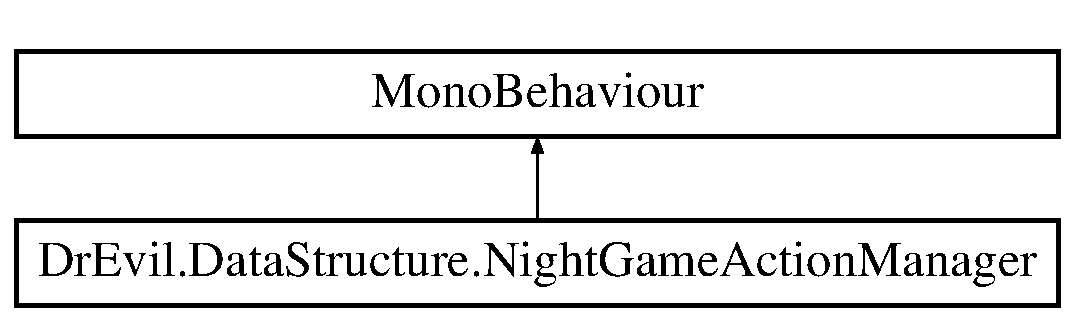
\includegraphics[height=2.000000cm]{class_dr_evil_1_1_data_structure_1_1_night_game_action_manager}
\end{center}
\end{figure}


\subsection{Detailed Description}
Loading the gamedata from json and generating tasks for a level to solve from the player 



The documentation for this class was generated from the following file\+:\begin{DoxyCompactItemize}
\item 
Gamejam\+Unity/\+Assets/\+Scripts/Night\+Game\+Action\+Manager.\+cs\end{DoxyCompactItemize}

\hypertarget{class_object_trigger}{}\section{Object\+Trigger Class Reference}
\label{class_object_trigger}\index{Object\+Trigger@{Object\+Trigger}}
Inheritance diagram for Object\+Trigger\+:\begin{figure}[H]
\begin{center}
\leavevmode
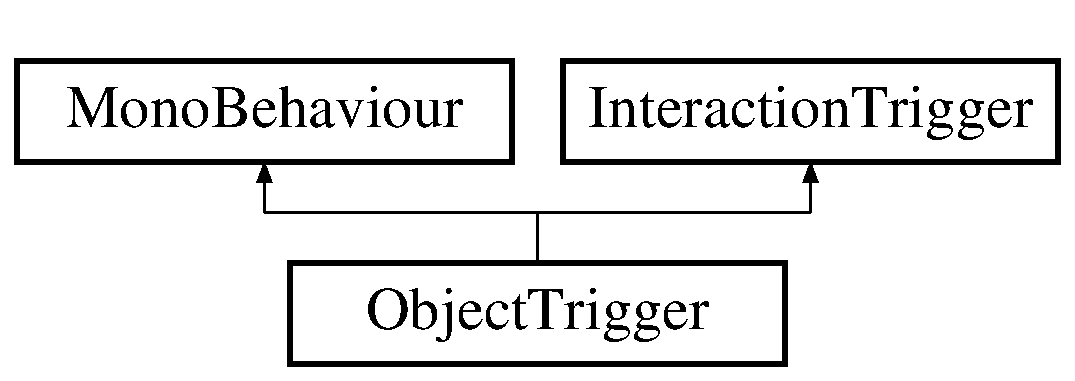
\includegraphics[height=2.000000cm]{class_object_trigger}
\end{center}
\end{figure}
\subsection*{Public Member Functions}
\begin{DoxyCompactItemize}
\item 
\mbox{\Hypertarget{class_object_trigger_a43ddb62721b7a3ed1a505a0090ab0f40}\label{class_object_trigger_a43ddb62721b7a3ed1a505a0090ab0f40}} 
void {\bfseries Action\+Completed} ()
\item 
\mbox{\Hypertarget{class_object_trigger_abfbb834f752e26cc6970d1d8a3b25b9a}\label{class_object_trigger_abfbb834f752e26cc6970d1d8a3b25b9a}} 
I\+Enumerator {\bfseries Trigger\+Action} (Action\+Complete Complete\+Callback)
\item 
\mbox{\Hypertarget{class_object_trigger_a6add425f2f6dbbe6e0fe4e30989c1b22}\label{class_object_trigger_a6add425f2f6dbbe6e0fe4e30989c1b22}} 
void {\bfseries Stop\+Action} ()
\end{DoxyCompactItemize}
\subsection*{Public Attributes}
\begin{DoxyCompactItemize}
\item 
\mbox{\Hypertarget{class_object_trigger_ab61adc34c964e2c0501916db38037b42}\label{class_object_trigger_ab61adc34c964e2c0501916db38037b42}} 
string {\bfseries Evil\+Action\+Identifier}
\item 
\mbox{\Hypertarget{class_object_trigger_a85ea5cd5631d10a550ead9f4df09326d}\label{class_object_trigger_a85ea5cd5631d10a550ead9f4df09326d}} 
\mbox{\hyperlink{class_evil_action}{Evil\+Action}} {\bfseries action\+Trigger}
\item 
\mbox{\Hypertarget{class_object_trigger_a3ce264e11707107314287b607db48744}\label{class_object_trigger_a3ce264e11707107314287b607db48744}} 
float {\bfseries trigger\+Complete\+Time}
\item 
\mbox{\Hypertarget{class_object_trigger_a16c2d109311b086fb1320e75c69ab36c}\label{class_object_trigger_a16c2d109311b086fb1320e75c69ab36c}} 
Animation {\bfseries anim}
\item 
\mbox{\Hypertarget{class_object_trigger_a7d96768a3ecc88b04b2b77e1e640f56d}\label{class_object_trigger_a7d96768a3ecc88b04b2b77e1e640f56d}} 
Audio\+Clip {\bfseries Success\+Audio\+Clip}
\item 
\mbox{\Hypertarget{class_object_trigger_a099869c27d33968b94f87c8f095a6891}\label{class_object_trigger_a099869c27d33968b94f87c8f095a6891}} 
bool {\bfseries is\+Solved}
\item 
\mbox{\Hypertarget{class_object_trigger_a068f1c5710685caaafceef6d7856f1fd}\label{class_object_trigger_a068f1c5710685caaafceef6d7856f1fd}} 
bool {\bfseries is\+Triggered}
\item 
\mbox{\Hypertarget{class_object_trigger_a220651fe5c130544bd82b56b326f8c30}\label{class_object_trigger_a220651fe5c130544bd82b56b326f8c30}} 
float {\bfseries holding\+Time}
\item 
\mbox{\Hypertarget{class_object_trigger_a817814665c0cbe18a37ff1082feb0a8f}\label{class_object_trigger_a817814665c0cbe18a37ff1082feb0a8f}} 
float {\bfseries holding\+Time\+Threshold}
\item 
\mbox{\Hypertarget{class_object_trigger_adca7ea0f51c98d9cd8fe6f17fa7c4643}\label{class_object_trigger_adca7ea0f51c98d9cd8fe6f17fa7c4643}} 
Game\+Object {\bfseries action\+Object}
\item 
\mbox{\Hypertarget{class_object_trigger_a8c1f6c7625fad597e8a8ff2f17bb4f01}\label{class_object_trigger_a8c1f6c7625fad597e8a8ff2f17bb4f01}} 
bool {\bfseries Is\+Failed} = false
\end{DoxyCompactItemize}


The documentation for this class was generated from the following file\+:\begin{DoxyCompactItemize}
\item 
Gamejam\+Unity/\+Assets/\+Scripts/\+Interactions/Object\+Trigger.\+cs\end{DoxyCompactItemize}

\hypertarget{class_person}{}\section{Person Class Reference}
\label{class_person}\index{Person@{Person}}
\subsection*{Properties}
\begin{DoxyCompactItemize}
\item 
\mbox{\Hypertarget{class_person_a0d6be70593995cc5124b92117e4a80b0}\label{class_person_a0d6be70593995cc5124b92117e4a80b0}} 
string {\bfseries Name}\hspace{0.3cm}{\ttfamily  \mbox{[}get, set\mbox{]}}
\item 
\mbox{\Hypertarget{class_person_a7c449dc4b8f61521e842b20e3625a7be}\label{class_person_a7c449dc4b8f61521e842b20e3625a7be}} 
string {\bfseries Alias}\hspace{0.3cm}{\ttfamily  \mbox{[}get, set\mbox{]}}
\item 
\mbox{\Hypertarget{class_person_a4d6848f2f7364bf79102b457ea9d5c1d}\label{class_person_a4d6848f2f7364bf79102b457ea9d5c1d}} 
int {\bfseries Age}\hspace{0.3cm}{\ttfamily  \mbox{[}get, set\mbox{]}}
\item 
\mbox{\Hypertarget{class_person_a79bbeb128635a64018bfd7b42e60cfa3}\label{class_person_a79bbeb128635a64018bfd7b42e60cfa3}} 
bool {\bfseries Finished}\hspace{0.3cm}{\ttfamily  \mbox{[}get, set\mbox{]}}
\item 
\mbox{\Hypertarget{class_person_a14c775d11b3deaefc4e5e0d30cc972cb}\label{class_person_a14c775d11b3deaefc4e5e0d30cc972cb}} 
bool {\bfseries Unlocked}\hspace{0.3cm}{\ttfamily  \mbox{[}get, set\mbox{]}}
\item 
\mbox{\Hypertarget{class_person_a2939cf47a6c1dca8ef627edbad1b7d8a}\label{class_person_a2939cf47a6c1dca8ef627edbad1b7d8a}} 
string {\bfseries Sprite\+Path\+In\+Resources}\hspace{0.3cm}{\ttfamily  \mbox{[}get, set\mbox{]}}
\item 
\mbox{\Hypertarget{class_person_ab90c7297b642e2bd80de84db346b673f}\label{class_person_ab90c7297b642e2bd80de84db346b673f}} 
List$<$ \mbox{\hyperlink{class_evil_action}{Evil\+Action}} $>$ {\bfseries Evil\+Action}\hspace{0.3cm}{\ttfamily  \mbox{[}get, set\mbox{]}}
\item 
\mbox{\Hypertarget{class_person_af84f42f43c9ff1bc45ca5b33102d71cd}\label{class_person_af84f42f43c9ff1bc45ca5b33102d71cd}} 
List$<$ \mbox{\hyperlink{class_evil_action}{Evil\+Action}} $>$ {\bfseries Solved\+Actions}\hspace{0.3cm}{\ttfamily  \mbox{[}get, set\mbox{]}}
\item 
\mbox{\Hypertarget{class_person_a04726feefce2dae1e5b1d4641a7e44d4}\label{class_person_a04726feefce2dae1e5b1d4641a7e44d4}} 
List$<$ \mbox{\hyperlink{class_therapy_story}{Therapy\+Story}} $>$ {\bfseries Therapy\+Story}\hspace{0.3cm}{\ttfamily  \mbox{[}get, set\mbox{]}}
\item 
\mbox{\Hypertarget{class_person_ab8970616a711e18b3647cd3904f401e5}\label{class_person_ab8970616a711e18b3647cd3904f401e5}} 
List$<$ \mbox{\hyperlink{class_review_story}{Review\+Story}} $>$ {\bfseries Review\+Story}\hspace{0.3cm}{\ttfamily  \mbox{[}get, set\mbox{]}}
\end{DoxyCompactItemize}


The documentation for this class was generated from the following file\+:\begin{DoxyCompactItemize}
\item 
Gamejam\+Unity/\+Assets/\+Scripts/\+Datastructure/Game\+World.\+cs\end{DoxyCompactItemize}

\hypertarget{class_review_story}{}\section{Review\+Story Class Reference}
\label{class_review_story}\index{Review\+Story@{Review\+Story}}
\subsection*{Properties}
\begin{DoxyCompactItemize}
\item 
\mbox{\Hypertarget{class_review_story_ad4d6897fe849b171697ab5816dd36009}\label{class_review_story_ad4d6897fe849b171697ab5816dd36009}} 
string {\bfseries Dialog\+Type}\hspace{0.3cm}{\ttfamily  \mbox{[}get, set\mbox{]}}
\item 
\mbox{\Hypertarget{class_review_story_ad7873b2f0e6602d0ce083d2cf11ef835}\label{class_review_story_ad7873b2f0e6602d0ce083d2cf11ef835}} 
string {\bfseries Actor}\hspace{0.3cm}{\ttfamily  \mbox{[}get, set\mbox{]}}
\item 
\mbox{\Hypertarget{class_review_story_a5f24c4aa8af6a38e9b4f247ce339e0fb}\label{class_review_story_a5f24c4aa8af6a38e9b4f247ce339e0fb}} 
string {\bfseries Message}\hspace{0.3cm}{\ttfamily  \mbox{[}get, set\mbox{]}}
\item 
\mbox{\Hypertarget{class_review_story_a92bee9ea9581da16b7d88092d3d508b5}\label{class_review_story_a92bee9ea9581da16b7d88092d3d508b5}} 
string {\bfseries Action\+Type}\hspace{0.3cm}{\ttfamily  \mbox{[}get, set\mbox{]}}
\item 
\mbox{\Hypertarget{class_review_story_ae94bf398a972a3046ec6b52eaeafcc3a}\label{class_review_story_ae94bf398a972a3046ec6b52eaeafcc3a}} 
string {\bfseries Identifier}\hspace{0.3cm}{\ttfamily  \mbox{[}get, set\mbox{]}}
\item 
\mbox{\Hypertarget{class_review_story_a4cde94205919a05dfddbdc0dc3f88f36}\label{class_review_story_a4cde94205919a05dfddbdc0dc3f88f36}} 
string {\bfseries Solved\+Message}\hspace{0.3cm}{\ttfamily  \mbox{[}get, set\mbox{]}}
\item 
\mbox{\Hypertarget{class_review_story_af28cd30c596761a48a6db8e4fd616071}\label{class_review_story_af28cd30c596761a48a6db8e4fd616071}} 
string {\bfseries Failed\+Message}\hspace{0.3cm}{\ttfamily  \mbox{[}get, set\mbox{]}}
\end{DoxyCompactItemize}


The documentation for this class was generated from the following file\+:\begin{DoxyCompactItemize}
\item 
Gamejam\+Unity/\+Assets/\+Scripts/\+Datastructure/Game\+World.\+cs\end{DoxyCompactItemize}

\hypertarget{class_root_object}{}\section{Root\+Object Class Reference}
\label{class_root_object}\index{Root\+Object@{Root\+Object}}
\subsection*{Properties}
\begin{DoxyCompactItemize}
\item 
\mbox{\Hypertarget{class_root_object_a46d9b6aec7770437b6bbbda31bb29bb4}\label{class_root_object_a46d9b6aec7770437b6bbbda31bb29bb4}} 
string {\bfseries Game}\hspace{0.3cm}{\ttfamily  \mbox{[}get, set\mbox{]}}
\item 
\mbox{\Hypertarget{class_root_object_ab04987285f5e56f095eb350a8a3959b5}\label{class_root_object_ab04987285f5e56f095eb350a8a3959b5}} 
int {\bfseries Revision}\hspace{0.3cm}{\ttfamily  \mbox{[}get, set\mbox{]}}
\item 
\mbox{\Hypertarget{class_root_object_af5c6c021486a3b6f75cc2f7e6e9b6745}\label{class_root_object_af5c6c021486a3b6f75cc2f7e6e9b6745}} 
List$<$ \mbox{\hyperlink{class_world}{World}} $>$ {\bfseries Worlds}\hspace{0.3cm}{\ttfamily  \mbox{[}get, set\mbox{]}}
\end{DoxyCompactItemize}


The documentation for this class was generated from the following file\+:\begin{DoxyCompactItemize}
\item 
Gamejam\+Unity/\+Assets/\+Scripts/\+Datastructure/Game\+World.\+cs\end{DoxyCompactItemize}

\hypertarget{class_screen_event_handler}{}\section{Screen\+Event\+Handler Class Reference}
\label{class_screen_event_handler}\index{Screen\+Event\+Handler@{Screen\+Event\+Handler}}
Inheritance diagram for Screen\+Event\+Handler\+:\begin{figure}[H]
\begin{center}
\leavevmode
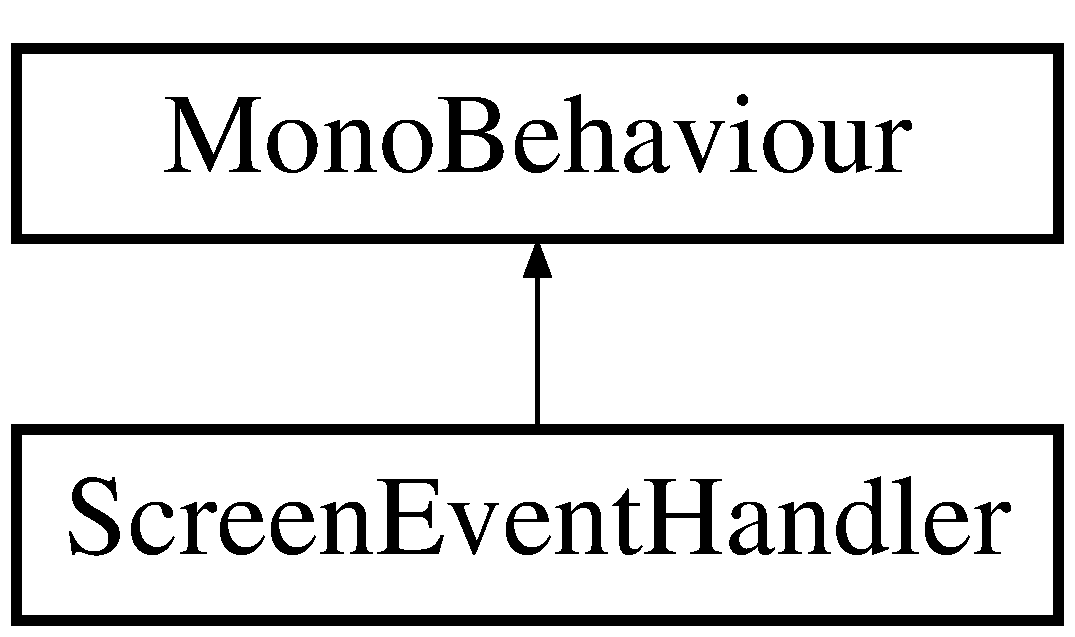
\includegraphics[height=2.000000cm]{class_screen_event_handler}
\end{center}
\end{figure}


The documentation for this class was generated from the following file\+:\begin{DoxyCompactItemize}
\item 
Gamejam\+Unity/\+Assets/Screen\+Event\+Handler.\+cs\end{DoxyCompactItemize}

\hypertarget{class_dr_evil_1_1_mechanics_1_1_screen_view_handler}{}\section{Dr\+Evil.\+Mechanics.\+Screen\+View\+Handler Class Reference}
\label{class_dr_evil_1_1_mechanics_1_1_screen_view_handler}\index{Dr\+Evil.\+Mechanics.\+Screen\+View\+Handler@{Dr\+Evil.\+Mechanics.\+Screen\+View\+Handler}}


This class handles everything regarding scenes and views and screens.  


Inheritance diagram for Dr\+Evil.\+Mechanics.\+Screen\+View\+Handler\+:\begin{figure}[H]
\begin{center}
\leavevmode
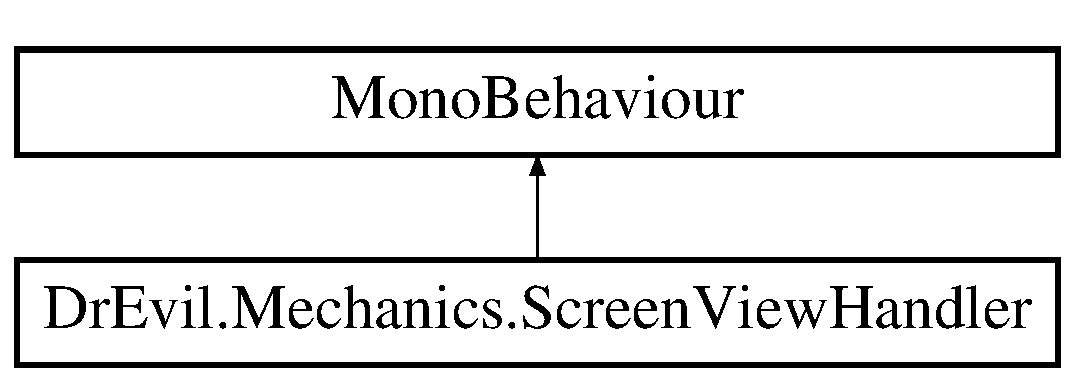
\includegraphics[height=2.000000cm]{class_dr_evil_1_1_mechanics_1_1_screen_view_handler}
\end{center}
\end{figure}
\subsection*{Public Member Functions}
\begin{DoxyCompactItemize}
\item 
void \mbox{\hyperlink{class_dr_evil_1_1_mechanics_1_1_screen_view_handler_a24540cf0bdc0ebccedd905a7ed53a471}{Skip\+Night\+Screen}} ()
\begin{DoxyCompactList}\small\item\em Method for skipping night loading screen \end{DoxyCompactList}\item 
I\+Enumerator \mbox{\hyperlink{class_dr_evil_1_1_mechanics_1_1_screen_view_handler_a19aa48d532b54e268c6be5288bbbfeaf}{Load\+Asynchonusly}} (string scene\+String)
\begin{DoxyCompactList}\small\item\em Load a level asyncronously \end{DoxyCompactList}\item 
void \mbox{\hyperlink{class_dr_evil_1_1_mechanics_1_1_screen_view_handler_a2e8c60d45fe706fe69b557c4d77625a3}{Finalize\+Level}} (bool is\+Accomplished)
\begin{DoxyCompactList}\small\item\em Finalize a level depending on solved status \end{DoxyCompactList}\item 
void \mbox{\hyperlink{class_dr_evil_1_1_mechanics_1_1_screen_view_handler_a29c4b74c77b7602740c3f90795321bf2}{Enter\+Night\+Scene}} ()
\begin{DoxyCompactList}\small\item\em Enter the night screen before accessing terror scene \end{DoxyCompactList}\item 
void \mbox{\hyperlink{class_dr_evil_1_1_mechanics_1_1_screen_view_handler_a51ae8bed2d6b3baf19756258c6b27b16}{Enter\+Mini\+Map\+Menu}} ()
\begin{DoxyCompactList}\small\item\em Show the Minimap Level overview \end{DoxyCompactList}\end{DoxyCompactItemize}
\subsection*{Public Attributes}
\begin{DoxyCompactItemize}
\item 
\mbox{\Hypertarget{class_dr_evil_1_1_mechanics_1_1_screen_view_handler_a108e61f2056f422e7019855531be0a56}\label{class_dr_evil_1_1_mechanics_1_1_screen_view_handler_a108e61f2056f422e7019855531be0a56}} 
\mbox{\hyperlink{class_dr_evil_1_1_mechanics_1_1_dialog_player}{Dialog\+Player}} {\bfseries Dialog\+Player}
\item 
\mbox{\Hypertarget{class_dr_evil_1_1_mechanics_1_1_screen_view_handler_a99bf477d5d85498daf46719d6e84de6c}\label{class_dr_evil_1_1_mechanics_1_1_screen_view_handler_a99bf477d5d85498daf46719d6e84de6c}} 
Game\+Object {\bfseries Start\+Screen}
\item 
\mbox{\Hypertarget{class_dr_evil_1_1_mechanics_1_1_screen_view_handler_adfd435c8f211676fc550e1f3a722ee43}\label{class_dr_evil_1_1_mechanics_1_1_screen_view_handler_adfd435c8f211676fc550e1f3a722ee43}} 
Button {\bfseries Enter\+Map\+Menu}
\item 
\mbox{\Hypertarget{class_dr_evil_1_1_mechanics_1_1_screen_view_handler_ae352a8a464b4316d34f7fe7c380638e1}\label{class_dr_evil_1_1_mechanics_1_1_screen_view_handler_ae352a8a464b4316d34f7fe7c380638e1}} 
Game\+Object {\bfseries Map\+View\+Game\+Object}
\item 
\mbox{\Hypertarget{class_dr_evil_1_1_mechanics_1_1_screen_view_handler_aaefbf2c7bee57785a22953d32e46e9bf}\label{class_dr_evil_1_1_mechanics_1_1_screen_view_handler_aaefbf2c7bee57785a22953d32e46e9bf}} 
Game\+Object {\bfseries Day\+Screen\+Game\+Object}
\item 
\mbox{\Hypertarget{class_dr_evil_1_1_mechanics_1_1_screen_view_handler_a36f7101c3b10a9fa5c12321065a4090a}\label{class_dr_evil_1_1_mechanics_1_1_screen_view_handler_a36f7101c3b10a9fa5c12321065a4090a}} 
\mbox{\hyperlink{class_dr_evil_1_1_visuals_1_1_u_i___sprite_animator}{U\+I\+\_\+\+Sprite\+Animator}} {\bfseries Animate\+Enter\+Therapy\+After\+Map}
\item 
\mbox{\Hypertarget{class_dr_evil_1_1_mechanics_1_1_screen_view_handler_a17a3fcbc786556349743c3a773a8607b}\label{class_dr_evil_1_1_mechanics_1_1_screen_view_handler_a17a3fcbc786556349743c3a773a8607b}} 
Game\+Object {\bfseries Night\+Screen}
\item 
\mbox{\Hypertarget{class_dr_evil_1_1_mechanics_1_1_screen_view_handler_ab3422612aca7afc3ae00e64803d10b4c}\label{class_dr_evil_1_1_mechanics_1_1_screen_view_handler_ab3422612aca7afc3ae00e64803d10b4c}} 
Game\+Object {\bfseries Level\+Accomplished\+Screen}
\item 
\mbox{\Hypertarget{class_dr_evil_1_1_mechanics_1_1_screen_view_handler_aec3e4add2f532723a55e1f28fb0ecd32}\label{class_dr_evil_1_1_mechanics_1_1_screen_view_handler_aec3e4add2f532723a55e1f28fb0ecd32}} 
Button {\bfseries Leave\+Finish\+V\+Btn}
\item 
\mbox{\Hypertarget{class_dr_evil_1_1_mechanics_1_1_screen_view_handler_a372e2777dad0e70941b8a7ee9128a926}\label{class_dr_evil_1_1_mechanics_1_1_screen_view_handler_a372e2777dad0e70941b8a7ee9128a926}} 
Game\+Object {\bfseries Level\+Failed\+Screen}
\item 
\mbox{\Hypertarget{class_dr_evil_1_1_mechanics_1_1_screen_view_handler_a19942a6dc923ab1c8b0606311f485df0}\label{class_dr_evil_1_1_mechanics_1_1_screen_view_handler_a19942a6dc923ab1c8b0606311f485df0}} 
Button {\bfseries Leave\+Un\+Finish\+V\+Btn}
\item 
\mbox{\Hypertarget{class_dr_evil_1_1_mechanics_1_1_screen_view_handler_ad86091f5532480fa462b80ce686e8df8}\label{class_dr_evil_1_1_mechanics_1_1_screen_view_handler_ad86091f5532480fa462b80ce686e8df8}} 
Button {\bfseries Skip\+Night\+Screen\+Btn}
\end{DoxyCompactItemize}
\subsection*{Static Public Attributes}
\begin{DoxyCompactItemize}
\item 
\mbox{\Hypertarget{class_dr_evil_1_1_mechanics_1_1_screen_view_handler_a257f83fe478544c684483bd3d87ee823}\label{class_dr_evil_1_1_mechanics_1_1_screen_view_handler_a257f83fe478544c684483bd3d87ee823}} 
static \mbox{\hyperlink{class_dr_evil_1_1_mechanics_1_1_screen_view_handler}{Screen\+View\+Handler}} {\bfseries instance}
\end{DoxyCompactItemize}


\subsection{Detailed Description}
This class handles everything regarding scenes and views and screens. 



\subsection{Member Function Documentation}
\mbox{\Hypertarget{class_dr_evil_1_1_mechanics_1_1_screen_view_handler_a51ae8bed2d6b3baf19756258c6b27b16}\label{class_dr_evil_1_1_mechanics_1_1_screen_view_handler_a51ae8bed2d6b3baf19756258c6b27b16}} 
\index{Dr\+Evil\+::\+Mechanics\+::\+Screen\+View\+Handler@{Dr\+Evil\+::\+Mechanics\+::\+Screen\+View\+Handler}!Enter\+Mini\+Map\+Menu@{Enter\+Mini\+Map\+Menu}}
\index{Enter\+Mini\+Map\+Menu@{Enter\+Mini\+Map\+Menu}!Dr\+Evil\+::\+Mechanics\+::\+Screen\+View\+Handler@{Dr\+Evil\+::\+Mechanics\+::\+Screen\+View\+Handler}}
\subsubsection{\texorpdfstring{Enter\+Mini\+Map\+Menu()}{EnterMiniMapMenu()}}
{\footnotesize\ttfamily void Dr\+Evil.\+Mechanics.\+Screen\+View\+Handler.\+Enter\+Mini\+Map\+Menu (\begin{DoxyParamCaption}{ }\end{DoxyParamCaption})\hspace{0.3cm}{\ttfamily [inline]}}



Show the Minimap Level overview 

\mbox{\Hypertarget{class_dr_evil_1_1_mechanics_1_1_screen_view_handler_a29c4b74c77b7602740c3f90795321bf2}\label{class_dr_evil_1_1_mechanics_1_1_screen_view_handler_a29c4b74c77b7602740c3f90795321bf2}} 
\index{Dr\+Evil\+::\+Mechanics\+::\+Screen\+View\+Handler@{Dr\+Evil\+::\+Mechanics\+::\+Screen\+View\+Handler}!Enter\+Night\+Scene@{Enter\+Night\+Scene}}
\index{Enter\+Night\+Scene@{Enter\+Night\+Scene}!Dr\+Evil\+::\+Mechanics\+::\+Screen\+View\+Handler@{Dr\+Evil\+::\+Mechanics\+::\+Screen\+View\+Handler}}
\subsubsection{\texorpdfstring{Enter\+Night\+Scene()}{EnterNightScene()}}
{\footnotesize\ttfamily void Dr\+Evil.\+Mechanics.\+Screen\+View\+Handler.\+Enter\+Night\+Scene (\begin{DoxyParamCaption}{ }\end{DoxyParamCaption})\hspace{0.3cm}{\ttfamily [inline]}}



Enter the night screen before accessing terror scene 

\mbox{\Hypertarget{class_dr_evil_1_1_mechanics_1_1_screen_view_handler_a2e8c60d45fe706fe69b557c4d77625a3}\label{class_dr_evil_1_1_mechanics_1_1_screen_view_handler_a2e8c60d45fe706fe69b557c4d77625a3}} 
\index{Dr\+Evil\+::\+Mechanics\+::\+Screen\+View\+Handler@{Dr\+Evil\+::\+Mechanics\+::\+Screen\+View\+Handler}!Finalize\+Level@{Finalize\+Level}}
\index{Finalize\+Level@{Finalize\+Level}!Dr\+Evil\+::\+Mechanics\+::\+Screen\+View\+Handler@{Dr\+Evil\+::\+Mechanics\+::\+Screen\+View\+Handler}}
\subsubsection{\texorpdfstring{Finalize\+Level()}{FinalizeLevel()}}
{\footnotesize\ttfamily void Dr\+Evil.\+Mechanics.\+Screen\+View\+Handler.\+Finalize\+Level (\begin{DoxyParamCaption}\item[{bool}]{is\+Accomplished }\end{DoxyParamCaption})\hspace{0.3cm}{\ttfamily [inline]}}



Finalize a level depending on solved status 


\begin{DoxyParams}{Parameters}
{\em is\+Accomplished} & \\
\hline
\end{DoxyParams}
\mbox{\Hypertarget{class_dr_evil_1_1_mechanics_1_1_screen_view_handler_a19aa48d532b54e268c6be5288bbbfeaf}\label{class_dr_evil_1_1_mechanics_1_1_screen_view_handler_a19aa48d532b54e268c6be5288bbbfeaf}} 
\index{Dr\+Evil\+::\+Mechanics\+::\+Screen\+View\+Handler@{Dr\+Evil\+::\+Mechanics\+::\+Screen\+View\+Handler}!Load\+Asynchonusly@{Load\+Asynchonusly}}
\index{Load\+Asynchonusly@{Load\+Asynchonusly}!Dr\+Evil\+::\+Mechanics\+::\+Screen\+View\+Handler@{Dr\+Evil\+::\+Mechanics\+::\+Screen\+View\+Handler}}
\subsubsection{\texorpdfstring{Load\+Asynchonusly()}{LoadAsynchonusly()}}
{\footnotesize\ttfamily I\+Enumerator Dr\+Evil.\+Mechanics.\+Screen\+View\+Handler.\+Load\+Asynchonusly (\begin{DoxyParamCaption}\item[{string}]{scene\+String }\end{DoxyParamCaption})\hspace{0.3cm}{\ttfamily [inline]}}



Load a level asyncronously 


\begin{DoxyParams}{Parameters}
{\em scene\+String} & \\
\hline
\end{DoxyParams}
\begin{DoxyReturn}{Returns}

\end{DoxyReturn}
\mbox{\Hypertarget{class_dr_evil_1_1_mechanics_1_1_screen_view_handler_a24540cf0bdc0ebccedd905a7ed53a471}\label{class_dr_evil_1_1_mechanics_1_1_screen_view_handler_a24540cf0bdc0ebccedd905a7ed53a471}} 
\index{Dr\+Evil\+::\+Mechanics\+::\+Screen\+View\+Handler@{Dr\+Evil\+::\+Mechanics\+::\+Screen\+View\+Handler}!Skip\+Night\+Screen@{Skip\+Night\+Screen}}
\index{Skip\+Night\+Screen@{Skip\+Night\+Screen}!Dr\+Evil\+::\+Mechanics\+::\+Screen\+View\+Handler@{Dr\+Evil\+::\+Mechanics\+::\+Screen\+View\+Handler}}
\subsubsection{\texorpdfstring{Skip\+Night\+Screen()}{SkipNightScreen()}}
{\footnotesize\ttfamily void Dr\+Evil.\+Mechanics.\+Screen\+View\+Handler.\+Skip\+Night\+Screen (\begin{DoxyParamCaption}{ }\end{DoxyParamCaption})\hspace{0.3cm}{\ttfamily [inline]}}



Method for skipping night loading screen 



The documentation for this class was generated from the following file\+:\begin{DoxyCompactItemize}
\item 
Gamejam\+Unity/\+Assets/Screen\+View\+Handler.\+cs\end{DoxyCompactItemize}

\hypertarget{class_dr_evil_1_1_testing_1_1_simulate_solved_actions}{}\section{Dr\+Evil.\+Testing.\+Simulate\+Solved\+Actions Class Reference}
\label{class_dr_evil_1_1_testing_1_1_simulate_solved_actions}\index{Dr\+Evil.\+Testing.\+Simulate\+Solved\+Actions@{Dr\+Evil.\+Testing.\+Simulate\+Solved\+Actions}}


\mbox{\hyperlink{namespace_dr_evil_1_1_testing}{Testing}} script to solve some interactions  


Inheritance diagram for Dr\+Evil.\+Testing.\+Simulate\+Solved\+Actions\+:\begin{figure}[H]
\begin{center}
\leavevmode
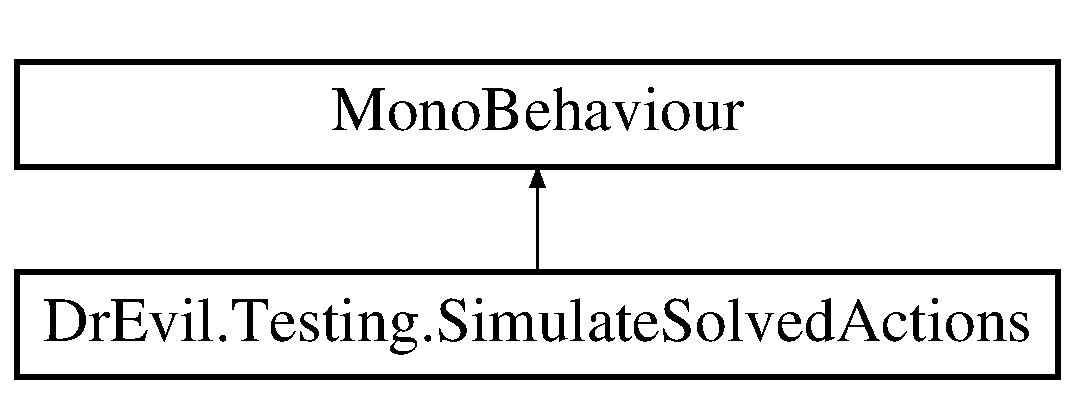
\includegraphics[height=2.000000cm]{class_dr_evil_1_1_testing_1_1_simulate_solved_actions}
\end{center}
\end{figure}
\subsection*{Public Attributes}
\begin{DoxyCompactItemize}
\item 
\mbox{\Hypertarget{class_dr_evil_1_1_testing_1_1_simulate_solved_actions_a53654f671e69ea2709f8d25a4bb50ea2}\label{class_dr_evil_1_1_testing_1_1_simulate_solved_actions_a53654f671e69ea2709f8d25a4bb50ea2}} 
bool {\bfseries solved\+Actions\+\_\+1}
\item 
\mbox{\Hypertarget{class_dr_evil_1_1_testing_1_1_simulate_solved_actions_a1a5d2f9cee3771edff92744a1ee5404e}\label{class_dr_evil_1_1_testing_1_1_simulate_solved_actions_a1a5d2f9cee3771edff92744a1ee5404e}} 
bool {\bfseries solved\+Actions\+\_\+2}
\item 
\mbox{\Hypertarget{class_dr_evil_1_1_testing_1_1_simulate_solved_actions_a243180a66c0e65e12fdad6a51c398181}\label{class_dr_evil_1_1_testing_1_1_simulate_solved_actions_a243180a66c0e65e12fdad6a51c398181}} 
bool {\bfseries solved\+Actions\+\_\+3}
\item 
\mbox{\Hypertarget{class_dr_evil_1_1_testing_1_1_simulate_solved_actions_a61d5ff24eb8b4671fa6bbdb69c76c300}\label{class_dr_evil_1_1_testing_1_1_simulate_solved_actions_a61d5ff24eb8b4671fa6bbdb69c76c300}} 
bool {\bfseries solved\+Actions\+\_\+4}
\end{DoxyCompactItemize}


\subsection{Detailed Description}
\mbox{\hyperlink{namespace_dr_evil_1_1_testing}{Testing}} script to solve some interactions 



The documentation for this class was generated from the following file\+:\begin{DoxyCompactItemize}
\item 
Gamejam\+Unity/\+Assets/Simulate\+Solved\+Actions.\+cs\end{DoxyCompactItemize}

\hypertarget{class_dr_evil_1_1_mechanics_1_1_sound_controller}{}\section{Dr\+Evil.\+Mechanics.\+Sound\+Controller Class Reference}
\label{class_dr_evil_1_1_mechanics_1_1_sound_controller}\index{Dr\+Evil.\+Mechanics.\+Sound\+Controller@{Dr\+Evil.\+Mechanics.\+Sound\+Controller}}
Inheritance diagram for Dr\+Evil.\+Mechanics.\+Sound\+Controller\+:\begin{figure}[H]
\begin{center}
\leavevmode
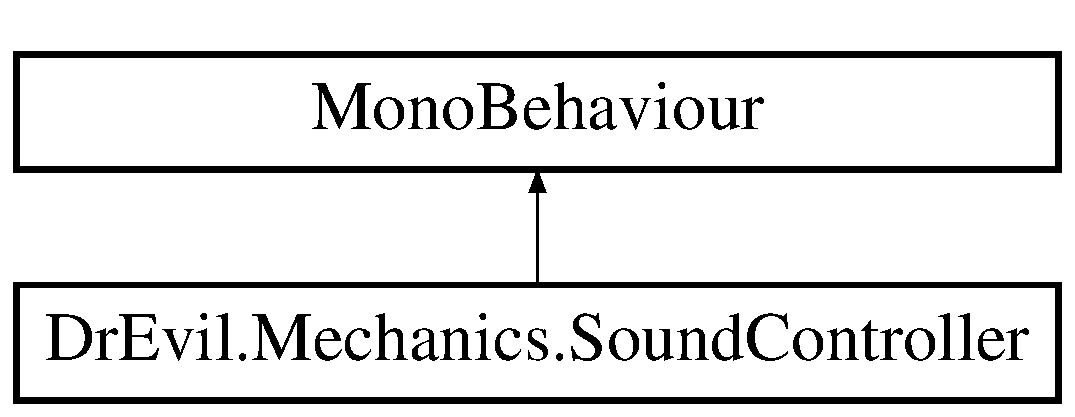
\includegraphics[height=2.000000cm]{class_dr_evil_1_1_mechanics_1_1_sound_controller}
\end{center}
\end{figure}
\subsection*{Public Member Functions}
\begin{DoxyCompactItemize}
\item 
void \mbox{\hyperlink{class_dr_evil_1_1_mechanics_1_1_sound_controller_a3f083cb0155e8bf4b03f38a355bf153a}{Stop\+All\+Sources}} ()
\begin{DoxyCompactList}\small\item\em Stop all sound sources \end{DoxyCompactList}\item 
void \mbox{\hyperlink{class_dr_evil_1_1_mechanics_1_1_sound_controller_af59c0ca5ff1b440a01c365372a762992}{Play\+Voice\+Loop}} (Audio\+Clip audio\+Clip)
\begin{DoxyCompactList}\small\item\em Play Audio\+Source Voice and let Loop \end{DoxyCompactList}\item 
void \mbox{\hyperlink{class_dr_evil_1_1_mechanics_1_1_sound_controller_a130372d19c0564c1119a1d94281f4b7e}{Stop\+Voice\+Loop}} (Audio\+Clip audio\+Clip)
\begin{DoxyCompactList}\small\item\em Stop Audio\+Source Voice\+Loop \end{DoxyCompactList}\item 
void \mbox{\hyperlink{class_dr_evil_1_1_mechanics_1_1_sound_controller_aead795046a4bac31ed5e8a69c5447e81}{Play\+Voice}} (Audio\+Clip audio\+Clip)
\begin{DoxyCompactList}\small\item\em Play Audio\+Source voice 1x \end{DoxyCompactList}\item 
void \mbox{\hyperlink{class_dr_evil_1_1_mechanics_1_1_sound_controller_aa5c3b26d880752cbe5f46fae6bab51db}{Play\+Music\+Loop}} (Audio\+Clip audio\+Clip)
\begin{DoxyCompactList}\small\item\em Play Audio\+Source Music in Loop \end{DoxyCompactList}\item 
void \mbox{\hyperlink{class_dr_evil_1_1_mechanics_1_1_sound_controller_afdb68fc451fcdc589ee969cf0a3d3090}{Stop\+Music\+Loop}} (Audio\+Clip audio\+Clip)
\begin{DoxyCompactList}\small\item\em Stop Audio\+Source Music Loop \end{DoxyCompactList}\end{DoxyCompactItemize}
\subsection*{Public Attributes}
\begin{DoxyCompactItemize}
\item 
Audio\+Clip \mbox{\hyperlink{class_dr_evil_1_1_mechanics_1_1_sound_controller_a1bf0d2d46e1805f3ccd105125f5225f8}{Dr\+Evil\+Laugh}}
\begin{DoxyCompactList}\small\item\em Hold all Voice an Music for Screenplay Let Play \& Stop all Audio\+Source \end{DoxyCompactList}\item 
\mbox{\Hypertarget{class_dr_evil_1_1_mechanics_1_1_sound_controller_a959aa03e8719b0f737bbc54cf9c98923}\label{class_dr_evil_1_1_mechanics_1_1_sound_controller_a959aa03e8719b0f737bbc54cf9c98923}} 
Audio\+Clip {\bfseries Dr\+Evil\+Talk}
\item 
\mbox{\Hypertarget{class_dr_evil_1_1_mechanics_1_1_sound_controller_a11cde4d0283aad25cbe4a4e0cdb126a8}\label{class_dr_evil_1_1_mechanics_1_1_sound_controller_a11cde4d0283aad25cbe4a4e0cdb126a8}} 
Audio\+Clip {\bfseries Dr\+Evil\+Un\+Solved}
\item 
\mbox{\Hypertarget{class_dr_evil_1_1_mechanics_1_1_sound_controller_a0c104b73a55f9aca5cdb0da12bb83c04}\label{class_dr_evil_1_1_mechanics_1_1_sound_controller_a0c104b73a55f9aca5cdb0da12bb83c04}} 
Audio\+Clip {\bfseries Achievement\+Sound}
\item 
\mbox{\Hypertarget{class_dr_evil_1_1_mechanics_1_1_sound_controller_aa9c558b3931e6a3dd98090ab7423a5ef}\label{class_dr_evil_1_1_mechanics_1_1_sound_controller_aa9c558b3931e6a3dd98090ab7423a5ef}} 
Audio\+Clip {\bfseries Patient\+Talk}
\item 
\mbox{\Hypertarget{class_dr_evil_1_1_mechanics_1_1_sound_controller_a50c35f4759ed2aab3dd10033922ea524}\label{class_dr_evil_1_1_mechanics_1_1_sound_controller_a50c35f4759ed2aab3dd10033922ea524}} 
Audio\+Clip {\bfseries Patient\+Scream}
\item 
\mbox{\Hypertarget{class_dr_evil_1_1_mechanics_1_1_sound_controller_a2f2b3559e95714516eb45342a994be31}\label{class_dr_evil_1_1_mechanics_1_1_sound_controller_a2f2b3559e95714516eb45342a994be31}} 
Audio\+Clip {\bfseries Start\+Screen\+Musik}
\item 
\mbox{\Hypertarget{class_dr_evil_1_1_mechanics_1_1_sound_controller_a1e545c755add6e5287ae2695daa581ce}\label{class_dr_evil_1_1_mechanics_1_1_sound_controller_a1e545c755add6e5287ae2695daa581ce}} 
Audio\+Clip {\bfseries Dialog\+Musik}
\item 
\mbox{\Hypertarget{class_dr_evil_1_1_mechanics_1_1_sound_controller_af6eb6340062c658b98925b99bfa1466a}\label{class_dr_evil_1_1_mechanics_1_1_sound_controller_af6eb6340062c658b98925b99bfa1466a}} 
Audio\+Clip {\bfseries Night\+Room\+Musik}
\item 
\mbox{\Hypertarget{class_dr_evil_1_1_mechanics_1_1_sound_controller_a2956864165cb78b38eb7e0ff2b4e5f04}\label{class_dr_evil_1_1_mechanics_1_1_sound_controller_a2956864165cb78b38eb7e0ff2b4e5f04}} 
Audio\+Clip {\bfseries door\+Open}
\item 
\mbox{\Hypertarget{class_dr_evil_1_1_mechanics_1_1_sound_controller_a79cd0f9efa40784fb196b24fb2eaa003}\label{class_dr_evil_1_1_mechanics_1_1_sound_controller_a79cd0f9efa40784fb196b24fb2eaa003}} 
Audio\+Source {\bfseries voice\+Loop}
\item 
\mbox{\Hypertarget{class_dr_evil_1_1_mechanics_1_1_sound_controller_a95db10148a9b5937e1f339851f4c43d4}\label{class_dr_evil_1_1_mechanics_1_1_sound_controller_a95db10148a9b5937e1f339851f4c43d4}} 
Audio\+Source {\bfseries voice}
\item 
\mbox{\Hypertarget{class_dr_evil_1_1_mechanics_1_1_sound_controller_a1b5748afc6fd6aab242da313b54e9d1d}\label{class_dr_evil_1_1_mechanics_1_1_sound_controller_a1b5748afc6fd6aab242da313b54e9d1d}} 
Audio\+Source {\bfseries musik}
\item 
\mbox{\Hypertarget{class_dr_evil_1_1_mechanics_1_1_sound_controller_a2da4a097ab1f46ffcaf6170baf60d072}\label{class_dr_evil_1_1_mechanics_1_1_sound_controller_a2da4a097ab1f46ffcaf6170baf60d072}} 
Audio\+Listener {\bfseries audio\+Listener}
\end{DoxyCompactItemize}


\subsection{Member Function Documentation}
\mbox{\Hypertarget{class_dr_evil_1_1_mechanics_1_1_sound_controller_aa5c3b26d880752cbe5f46fae6bab51db}\label{class_dr_evil_1_1_mechanics_1_1_sound_controller_aa5c3b26d880752cbe5f46fae6bab51db}} 
\index{Dr\+Evil\+::\+Mechanics\+::\+Sound\+Controller@{Dr\+Evil\+::\+Mechanics\+::\+Sound\+Controller}!Play\+Music\+Loop@{Play\+Music\+Loop}}
\index{Play\+Music\+Loop@{Play\+Music\+Loop}!Dr\+Evil\+::\+Mechanics\+::\+Sound\+Controller@{Dr\+Evil\+::\+Mechanics\+::\+Sound\+Controller}}
\subsubsection{\texorpdfstring{Play\+Music\+Loop()}{PlayMusicLoop()}}
{\footnotesize\ttfamily void Dr\+Evil.\+Mechanics.\+Sound\+Controller.\+Play\+Music\+Loop (\begin{DoxyParamCaption}\item[{Audio\+Clip}]{audio\+Clip }\end{DoxyParamCaption})\hspace{0.3cm}{\ttfamily [inline]}}



Play Audio\+Source Music in Loop 


\begin{DoxyParams}{Parameters}
{\em audio\+Clip} & \\
\hline
\end{DoxyParams}
\mbox{\Hypertarget{class_dr_evil_1_1_mechanics_1_1_sound_controller_aead795046a4bac31ed5e8a69c5447e81}\label{class_dr_evil_1_1_mechanics_1_1_sound_controller_aead795046a4bac31ed5e8a69c5447e81}} 
\index{Dr\+Evil\+::\+Mechanics\+::\+Sound\+Controller@{Dr\+Evil\+::\+Mechanics\+::\+Sound\+Controller}!Play\+Voice@{Play\+Voice}}
\index{Play\+Voice@{Play\+Voice}!Dr\+Evil\+::\+Mechanics\+::\+Sound\+Controller@{Dr\+Evil\+::\+Mechanics\+::\+Sound\+Controller}}
\subsubsection{\texorpdfstring{Play\+Voice()}{PlayVoice()}}
{\footnotesize\ttfamily void Dr\+Evil.\+Mechanics.\+Sound\+Controller.\+Play\+Voice (\begin{DoxyParamCaption}\item[{Audio\+Clip}]{audio\+Clip }\end{DoxyParamCaption})\hspace{0.3cm}{\ttfamily [inline]}}



Play Audio\+Source voice 1x 


\begin{DoxyParams}{Parameters}
{\em audio\+Clip} & \\
\hline
\end{DoxyParams}
\mbox{\Hypertarget{class_dr_evil_1_1_mechanics_1_1_sound_controller_af59c0ca5ff1b440a01c365372a762992}\label{class_dr_evil_1_1_mechanics_1_1_sound_controller_af59c0ca5ff1b440a01c365372a762992}} 
\index{Dr\+Evil\+::\+Mechanics\+::\+Sound\+Controller@{Dr\+Evil\+::\+Mechanics\+::\+Sound\+Controller}!Play\+Voice\+Loop@{Play\+Voice\+Loop}}
\index{Play\+Voice\+Loop@{Play\+Voice\+Loop}!Dr\+Evil\+::\+Mechanics\+::\+Sound\+Controller@{Dr\+Evil\+::\+Mechanics\+::\+Sound\+Controller}}
\subsubsection{\texorpdfstring{Play\+Voice\+Loop()}{PlayVoiceLoop()}}
{\footnotesize\ttfamily void Dr\+Evil.\+Mechanics.\+Sound\+Controller.\+Play\+Voice\+Loop (\begin{DoxyParamCaption}\item[{Audio\+Clip}]{audio\+Clip }\end{DoxyParamCaption})\hspace{0.3cm}{\ttfamily [inline]}}



Play Audio\+Source Voice and let Loop 


\begin{DoxyParams}{Parameters}
{\em audio\+Clip} & \\
\hline
\end{DoxyParams}
\mbox{\Hypertarget{class_dr_evil_1_1_mechanics_1_1_sound_controller_a3f083cb0155e8bf4b03f38a355bf153a}\label{class_dr_evil_1_1_mechanics_1_1_sound_controller_a3f083cb0155e8bf4b03f38a355bf153a}} 
\index{Dr\+Evil\+::\+Mechanics\+::\+Sound\+Controller@{Dr\+Evil\+::\+Mechanics\+::\+Sound\+Controller}!Stop\+All\+Sources@{Stop\+All\+Sources}}
\index{Stop\+All\+Sources@{Stop\+All\+Sources}!Dr\+Evil\+::\+Mechanics\+::\+Sound\+Controller@{Dr\+Evil\+::\+Mechanics\+::\+Sound\+Controller}}
\subsubsection{\texorpdfstring{Stop\+All\+Sources()}{StopAllSources()}}
{\footnotesize\ttfamily void Dr\+Evil.\+Mechanics.\+Sound\+Controller.\+Stop\+All\+Sources (\begin{DoxyParamCaption}{ }\end{DoxyParamCaption})\hspace{0.3cm}{\ttfamily [inline]}}



Stop all sound sources 

\mbox{\Hypertarget{class_dr_evil_1_1_mechanics_1_1_sound_controller_afdb68fc451fcdc589ee969cf0a3d3090}\label{class_dr_evil_1_1_mechanics_1_1_sound_controller_afdb68fc451fcdc589ee969cf0a3d3090}} 
\index{Dr\+Evil\+::\+Mechanics\+::\+Sound\+Controller@{Dr\+Evil\+::\+Mechanics\+::\+Sound\+Controller}!Stop\+Music\+Loop@{Stop\+Music\+Loop}}
\index{Stop\+Music\+Loop@{Stop\+Music\+Loop}!Dr\+Evil\+::\+Mechanics\+::\+Sound\+Controller@{Dr\+Evil\+::\+Mechanics\+::\+Sound\+Controller}}
\subsubsection{\texorpdfstring{Stop\+Music\+Loop()}{StopMusicLoop()}}
{\footnotesize\ttfamily void Dr\+Evil.\+Mechanics.\+Sound\+Controller.\+Stop\+Music\+Loop (\begin{DoxyParamCaption}\item[{Audio\+Clip}]{audio\+Clip }\end{DoxyParamCaption})\hspace{0.3cm}{\ttfamily [inline]}}



Stop Audio\+Source Music Loop 


\begin{DoxyParams}{Parameters}
{\em audio\+Clip} & \\
\hline
\end{DoxyParams}
\mbox{\Hypertarget{class_dr_evil_1_1_mechanics_1_1_sound_controller_a130372d19c0564c1119a1d94281f4b7e}\label{class_dr_evil_1_1_mechanics_1_1_sound_controller_a130372d19c0564c1119a1d94281f4b7e}} 
\index{Dr\+Evil\+::\+Mechanics\+::\+Sound\+Controller@{Dr\+Evil\+::\+Mechanics\+::\+Sound\+Controller}!Stop\+Voice\+Loop@{Stop\+Voice\+Loop}}
\index{Stop\+Voice\+Loop@{Stop\+Voice\+Loop}!Dr\+Evil\+::\+Mechanics\+::\+Sound\+Controller@{Dr\+Evil\+::\+Mechanics\+::\+Sound\+Controller}}
\subsubsection{\texorpdfstring{Stop\+Voice\+Loop()}{StopVoiceLoop()}}
{\footnotesize\ttfamily void Dr\+Evil.\+Mechanics.\+Sound\+Controller.\+Stop\+Voice\+Loop (\begin{DoxyParamCaption}\item[{Audio\+Clip}]{audio\+Clip }\end{DoxyParamCaption})\hspace{0.3cm}{\ttfamily [inline]}}



Stop Audio\+Source Voice\+Loop 


\begin{DoxyParams}{Parameters}
{\em audio\+Clip} & \\
\hline
\end{DoxyParams}


\subsection{Member Data Documentation}
\mbox{\Hypertarget{class_dr_evil_1_1_mechanics_1_1_sound_controller_a1bf0d2d46e1805f3ccd105125f5225f8}\label{class_dr_evil_1_1_mechanics_1_1_sound_controller_a1bf0d2d46e1805f3ccd105125f5225f8}} 
\index{Dr\+Evil\+::\+Mechanics\+::\+Sound\+Controller@{Dr\+Evil\+::\+Mechanics\+::\+Sound\+Controller}!Dr\+Evil\+Laugh@{Dr\+Evil\+Laugh}}
\index{Dr\+Evil\+Laugh@{Dr\+Evil\+Laugh}!Dr\+Evil\+::\+Mechanics\+::\+Sound\+Controller@{Dr\+Evil\+::\+Mechanics\+::\+Sound\+Controller}}
\subsubsection{\texorpdfstring{Dr\+Evil\+Laugh}{DrEvilLaugh}}
{\footnotesize\ttfamily Audio\+Clip Dr\+Evil.\+Mechanics.\+Sound\+Controller.\+Dr\+Evil\+Laugh}



Hold all Voice an Music for Screenplay Let Play \& Stop all Audio\+Source 



The documentation for this class was generated from the following file\+:\begin{DoxyCompactItemize}
\item 
Gamejam\+Unity/\+Assets/\+Scripts/Sound\+Controller.\+cs\end{DoxyCompactItemize}

\hypertarget{class_dr_evil_1_1_mechanics_1_1_terror_level_controller}{}\section{Dr\+Evil.\+Mechanics.\+Terror\+Level\+Controller Class Reference}
\label{class_dr_evil_1_1_mechanics_1_1_terror_level_controller}\index{Dr\+Evil.\+Mechanics.\+Terror\+Level\+Controller@{Dr\+Evil.\+Mechanics.\+Terror\+Level\+Controller}}


This Class handles whole mechanics of the terror room  


Inheritance diagram for Dr\+Evil.\+Mechanics.\+Terror\+Level\+Controller\+:\begin{figure}[H]
\begin{center}
\leavevmode
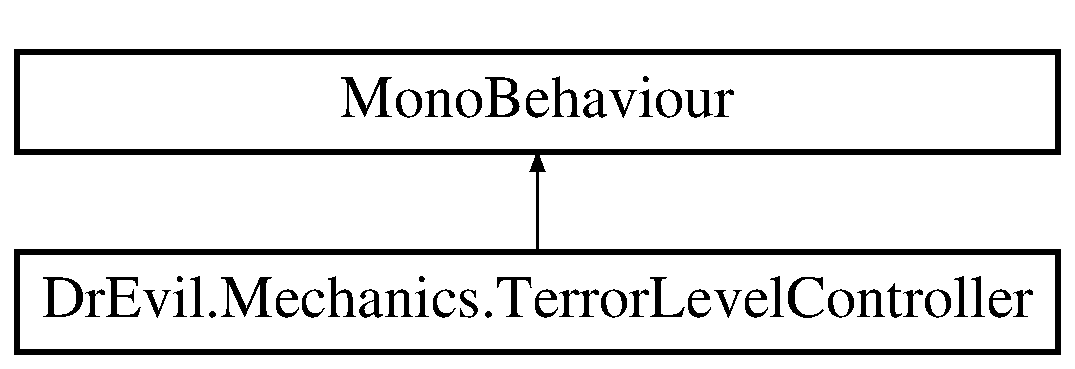
\includegraphics[height=2.000000cm]{class_dr_evil_1_1_mechanics_1_1_terror_level_controller}
\end{center}
\end{figure}
\subsection*{Public Member Functions}
\begin{DoxyCompactItemize}
\item 
\mbox{\Hypertarget{class_dr_evil_1_1_mechanics_1_1_terror_level_controller_a7e2676666d6e8bf3a853ebafc694f31e}\label{class_dr_evil_1_1_mechanics_1_1_terror_level_controller_a7e2676666d6e8bf3a853ebafc694f31e}} 
void {\bfseries Init} ()
\item 
void \mbox{\hyperlink{class_dr_evil_1_1_mechanics_1_1_terror_level_controller_a8d383e0849fbd683b2032658a751a783}{Add\+Scratch\+Action}} (\mbox{\hyperlink{class_evil_action}{Evil\+Action}} scratch\+Evil\+Action)
\begin{DoxyCompactList}\small\item\em Add a scratch event to the game if it is defined in the game\+Data \end{DoxyCompactList}\item 
void \mbox{\hyperlink{class_dr_evil_1_1_mechanics_1_1_terror_level_controller_a4c48f71b3f4881fd082d2a823aa19464}{Add\+Voice\+Action}} (\mbox{\hyperlink{class_evil_action}{Evil\+Action}} voice\+Evil\+Action)
\begin{DoxyCompactList}\small\item\em Add a voice event to the game if it is defined in the game\+Data \end{DoxyCompactList}\item 
I\+Enumerator \mbox{\hyperlink{class_dr_evil_1_1_mechanics_1_1_terror_level_controller_a0ababae78433f3aed00a7a871f3526fc}{Play\+Failed\+Sound}} ()
\begin{DoxyCompactList}\small\item\em Play a failed sound feedback from the patient \end{DoxyCompactList}\end{DoxyCompactItemize}
\subsection*{Public Attributes}
\begin{DoxyCompactItemize}
\item 
\mbox{\Hypertarget{class_dr_evil_1_1_mechanics_1_1_terror_level_controller_a3f346e3b9e677f38dff3a6c33576526b}\label{class_dr_evil_1_1_mechanics_1_1_terror_level_controller_a3f346e3b9e677f38dff3a6c33576526b}} 
int {\bfseries max\+Fail\+Attempts} = 5
\item 
\mbox{\Hypertarget{class_dr_evil_1_1_mechanics_1_1_terror_level_controller_a6c98e3c7c3c2b93c82b4dee5bb3594b4}\label{class_dr_evil_1_1_mechanics_1_1_terror_level_controller_a6c98e3c7c3c2b93c82b4dee5bb3594b4}} 
float {\bfseries fail\+Attempt\+Wait\+Time} = 1.\+5f
\item 
\mbox{\Hypertarget{class_dr_evil_1_1_mechanics_1_1_terror_level_controller_afb66ad1d935e72eeee1b3161f2938a7a}\label{class_dr_evil_1_1_mechanics_1_1_terror_level_controller_afb66ad1d935e72eeee1b3161f2938a7a}} 
bool {\bfseries has\+User\+Swiped}
\item 
\mbox{\Hypertarget{class_dr_evil_1_1_mechanics_1_1_terror_level_controller_a6897cd0203f2ef41ef46fa2a7ac22faa}\label{class_dr_evil_1_1_mechanics_1_1_terror_level_controller_a6897cd0203f2ef41ef46fa2a7ac22faa}} 
Audio\+Source {\bfseries level\+Audio\+Source}
\item 
\mbox{\Hypertarget{class_dr_evil_1_1_mechanics_1_1_terror_level_controller_a7d96119b3e69dfcfd4b05c5cc4d98659}\label{class_dr_evil_1_1_mechanics_1_1_terror_level_controller_a7d96119b3e69dfcfd4b05c5cc4d98659}} 
Audio\+Source {\bfseries Voice\+Audio\+Source}
\item 
\mbox{\Hypertarget{class_dr_evil_1_1_mechanics_1_1_terror_level_controller_a433abcb89175595b9e621de20347a59a}\label{class_dr_evil_1_1_mechanics_1_1_terror_level_controller_a433abcb89175595b9e621de20347a59a}} 
Audio\+Clip {\bfseries Voice\+Audio\+Clip}
\item 
\mbox{\Hypertarget{class_dr_evil_1_1_mechanics_1_1_terror_level_controller_aeab14cd3a88b08612f84bae4edb0cdbc}\label{class_dr_evil_1_1_mechanics_1_1_terror_level_controller_aeab14cd3a88b08612f84bae4edb0cdbc}} 
List$<$ Audio\+Clip $>$ {\bfseries Failed\+Clips}
\item 
\mbox{\Hypertarget{class_dr_evil_1_1_mechanics_1_1_terror_level_controller_a11e7a2308c6085d21928d71cac93cc92}\label{class_dr_evil_1_1_mechanics_1_1_terror_level_controller_a11e7a2308c6085d21928d71cac93cc92}} 
int {\bfseries failed\+Clip\+Index} = -\/1
\end{DoxyCompactItemize}
\subsection*{Static Public Attributes}
\begin{DoxyCompactItemize}
\item 
\mbox{\Hypertarget{class_dr_evil_1_1_mechanics_1_1_terror_level_controller_a7291cb2b49c2e1153262c70e09915d45}\label{class_dr_evil_1_1_mechanics_1_1_terror_level_controller_a7291cb2b49c2e1153262c70e09915d45}} 
static \mbox{\hyperlink{class_dr_evil_1_1_mechanics_1_1_terror_level_controller}{Terror\+Level\+Controller}} {\bfseries instance}
\end{DoxyCompactItemize}


\subsection{Detailed Description}
This Class handles whole mechanics of the terror room 



\subsection{Member Function Documentation}
\mbox{\Hypertarget{class_dr_evil_1_1_mechanics_1_1_terror_level_controller_a8d383e0849fbd683b2032658a751a783}\label{class_dr_evil_1_1_mechanics_1_1_terror_level_controller_a8d383e0849fbd683b2032658a751a783}} 
\index{Dr\+Evil\+::\+Mechanics\+::\+Terror\+Level\+Controller@{Dr\+Evil\+::\+Mechanics\+::\+Terror\+Level\+Controller}!Add\+Scratch\+Action@{Add\+Scratch\+Action}}
\index{Add\+Scratch\+Action@{Add\+Scratch\+Action}!Dr\+Evil\+::\+Mechanics\+::\+Terror\+Level\+Controller@{Dr\+Evil\+::\+Mechanics\+::\+Terror\+Level\+Controller}}
\subsubsection{\texorpdfstring{Add\+Scratch\+Action()}{AddScratchAction()}}
{\footnotesize\ttfamily void Dr\+Evil.\+Mechanics.\+Terror\+Level\+Controller.\+Add\+Scratch\+Action (\begin{DoxyParamCaption}\item[{\mbox{\hyperlink{class_evil_action}{Evil\+Action}}}]{scratch\+Evil\+Action }\end{DoxyParamCaption})\hspace{0.3cm}{\ttfamily [inline]}}



Add a scratch event to the game if it is defined in the game\+Data 


\begin{DoxyParams}{Parameters}
{\em scratch\+Evil\+Action} & \\
\hline
\end{DoxyParams}
\mbox{\Hypertarget{class_dr_evil_1_1_mechanics_1_1_terror_level_controller_a4c48f71b3f4881fd082d2a823aa19464}\label{class_dr_evil_1_1_mechanics_1_1_terror_level_controller_a4c48f71b3f4881fd082d2a823aa19464}} 
\index{Dr\+Evil\+::\+Mechanics\+::\+Terror\+Level\+Controller@{Dr\+Evil\+::\+Mechanics\+::\+Terror\+Level\+Controller}!Add\+Voice\+Action@{Add\+Voice\+Action}}
\index{Add\+Voice\+Action@{Add\+Voice\+Action}!Dr\+Evil\+::\+Mechanics\+::\+Terror\+Level\+Controller@{Dr\+Evil\+::\+Mechanics\+::\+Terror\+Level\+Controller}}
\subsubsection{\texorpdfstring{Add\+Voice\+Action()}{AddVoiceAction()}}
{\footnotesize\ttfamily void Dr\+Evil.\+Mechanics.\+Terror\+Level\+Controller.\+Add\+Voice\+Action (\begin{DoxyParamCaption}\item[{\mbox{\hyperlink{class_evil_action}{Evil\+Action}}}]{voice\+Evil\+Action }\end{DoxyParamCaption})\hspace{0.3cm}{\ttfamily [inline]}}



Add a voice event to the game if it is defined in the game\+Data 


\begin{DoxyParams}{Parameters}
{\em voice\+Evil\+Action} & \\
\hline
\end{DoxyParams}
\mbox{\Hypertarget{class_dr_evil_1_1_mechanics_1_1_terror_level_controller_a0ababae78433f3aed00a7a871f3526fc}\label{class_dr_evil_1_1_mechanics_1_1_terror_level_controller_a0ababae78433f3aed00a7a871f3526fc}} 
\index{Dr\+Evil\+::\+Mechanics\+::\+Terror\+Level\+Controller@{Dr\+Evil\+::\+Mechanics\+::\+Terror\+Level\+Controller}!Play\+Failed\+Sound@{Play\+Failed\+Sound}}
\index{Play\+Failed\+Sound@{Play\+Failed\+Sound}!Dr\+Evil\+::\+Mechanics\+::\+Terror\+Level\+Controller@{Dr\+Evil\+::\+Mechanics\+::\+Terror\+Level\+Controller}}
\subsubsection{\texorpdfstring{Play\+Failed\+Sound()}{PlayFailedSound()}}
{\footnotesize\ttfamily I\+Enumerator Dr\+Evil.\+Mechanics.\+Terror\+Level\+Controller.\+Play\+Failed\+Sound (\begin{DoxyParamCaption}{ }\end{DoxyParamCaption})\hspace{0.3cm}{\ttfamily [inline]}}



Play a failed sound feedback from the patient 

\begin{DoxyReturn}{Returns}

\end{DoxyReturn}


The documentation for this class was generated from the following file\+:\begin{DoxyCompactItemize}
\item 
Gamejam\+Unity/\+Assets/\+Scripts/Terror\+Level\+Controller.\+cs\end{DoxyCompactItemize}

\hypertarget{class_therapy_story}{}\section{Therapy\+Story Class Reference}
\label{class_therapy_story}\index{Therapy\+Story@{Therapy\+Story}}
\subsection*{Properties}
\begin{DoxyCompactItemize}
\item 
\mbox{\Hypertarget{class_therapy_story_a80a4755060f380596ef774273791049e}\label{class_therapy_story_a80a4755060f380596ef774273791049e}} 
string {\bfseries Dialoge\+Type}\hspace{0.3cm}{\ttfamily  \mbox{[}get, set\mbox{]}}
\item 
\mbox{\Hypertarget{class_therapy_story_aa8f7ab54623e3a89a4f708a47cdc181b}\label{class_therapy_story_aa8f7ab54623e3a89a4f708a47cdc181b}} 
string {\bfseries Actor}\hspace{0.3cm}{\ttfamily  \mbox{[}get, set\mbox{]}}
\item 
\mbox{\Hypertarget{class_therapy_story_a4301ee229988d83c34be7ed83d189206}\label{class_therapy_story_a4301ee229988d83c34be7ed83d189206}} 
string {\bfseries Message}\hspace{0.3cm}{\ttfamily  \mbox{[}get, set\mbox{]}}
\item 
\mbox{\Hypertarget{class_therapy_story_a952b404f07cdc2a6f5562c3ff7852ab0}\label{class_therapy_story_a952b404f07cdc2a6f5562c3ff7852ab0}} 
string {\bfseries Action\+Type}\hspace{0.3cm}{\ttfamily  \mbox{[}get, set\mbox{]}}
\end{DoxyCompactItemize}


The documentation for this class was generated from the following file\+:\begin{DoxyCompactItemize}
\item 
Gamejam\+Unity/\+Assets/\+Scripts/\+Datastructure/Game\+World.\+cs\end{DoxyCompactItemize}

\hypertarget{struct_threshold}{}\section{Threshold Struct Reference}
\label{struct_threshold}\index{Threshold@{Threshold}}
\subsection*{Public Attributes}
\begin{DoxyCompactItemize}
\item 
\mbox{\Hypertarget{struct_threshold_a50400d3879b9a6bd7f3efa417b16a26e}\label{struct_threshold_a50400d3879b9a6bd7f3efa417b16a26e}} 
Threshold\+Level {\bfseries level}
\item 
\mbox{\Hypertarget{struct_threshold_aa48c4a9c221f68bab66c6d3862a262c0}\label{struct_threshold_aa48c4a9c221f68bab66c6d3862a262c0}} 
float {\bfseries amount}
\end{DoxyCompactItemize}


The documentation for this struct was generated from the following file\+:\begin{DoxyCompactItemize}
\item 
Gamejam\+Unity/\+Assets/\+Scripts/Mobile\+Input.\+cs\end{DoxyCompactItemize}

\hypertarget{class_dr_evil_1_1_visuals_1_1_u_i___graphic___rescaler}{}\section{Dr\+Evil.\+Visuals.\+U\+I\+\_\+\+Graphic\+\_\+\+Rescaler Class Reference}
\label{class_dr_evil_1_1_visuals_1_1_u_i___graphic___rescaler}\index{Dr\+Evil.\+Visuals.\+U\+I\+\_\+\+Graphic\+\_\+\+Rescaler@{Dr\+Evil.\+Visuals.\+U\+I\+\_\+\+Graphic\+\_\+\+Rescaler}}
Inheritance diagram for Dr\+Evil.\+Visuals.\+U\+I\+\_\+\+Graphic\+\_\+\+Rescaler\+:\begin{figure}[H]
\begin{center}
\leavevmode
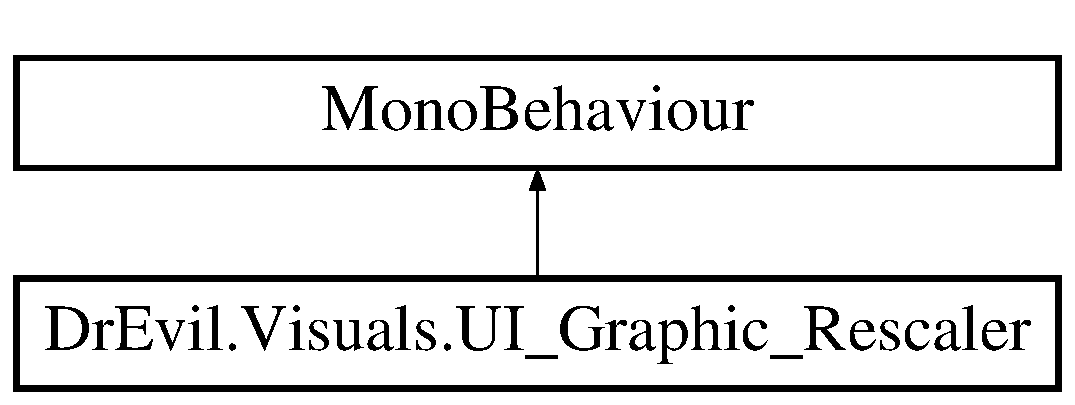
\includegraphics[height=2.000000cm]{class_dr_evil_1_1_visuals_1_1_u_i___graphic___rescaler}
\end{center}
\end{figure}
\subsection*{Public Member Functions}
\begin{DoxyCompactItemize}
\item 
\mbox{\Hypertarget{class_dr_evil_1_1_visuals_1_1_u_i___graphic___rescaler_a10a56121ca5e03efac5eb4fa24c79817}\label{class_dr_evil_1_1_visuals_1_1_u_i___graphic___rescaler_a10a56121ca5e03efac5eb4fa24c79817}} 
void {\bfseries Init} ()
\item 
void \mbox{\hyperlink{class_dr_evil_1_1_visuals_1_1_u_i___graphic___rescaler_a6c819e24dee525765ce354f39e0478ea}{Rescale\+Image\+Based\+On\+Height}} ()
\begin{DoxyCompactList}\small\item\em Rescale the ui element depending on the height value \end{DoxyCompactList}\item 
void \mbox{\hyperlink{class_dr_evil_1_1_visuals_1_1_u_i___graphic___rescaler_abb10e3ebe643e7ed763002f246062f3f}{rescale\+Image\+Based\+On\+Width}} ()
\begin{DoxyCompactList}\small\item\em Rescale the ui element depending on the width value \end{DoxyCompactList}\item 
void \mbox{\hyperlink{class_dr_evil_1_1_visuals_1_1_u_i___graphic___rescaler_a8b851fe76ba2a6d41b0b156baa274251}{set\+Percentage\+Offset}} ()
\begin{DoxyCompactList}\small\item\em Apply the percante offset to the ui element \end{DoxyCompactList}\item 
float \mbox{\hyperlink{class_dr_evil_1_1_visuals_1_1_u_i___graphic___rescaler_a5656984c54269ca385bd21e559929fc6}{Get\+Aspect\+Ratio\+Height}} ()
\begin{DoxyCompactList}\small\item\em Get Aspect ratio depending on height od the device size \end{DoxyCompactList}\item 
float \mbox{\hyperlink{class_dr_evil_1_1_visuals_1_1_u_i___graphic___rescaler_a736d14065b635502d82e3a12f23e0a76}{Get\+Aspect\+Ratio\+Width}} ()
\begin{DoxyCompactList}\small\item\em Get Aspect ratio depending on width od the device size \end{DoxyCompactList}\item 
float \mbox{\hyperlink{class_dr_evil_1_1_visuals_1_1_u_i___graphic___rescaler_a15a7abe2fa585e1de10bbe42194b3ff7}{Get\+Percentage\+Width}} (float percentage)
\begin{DoxyCompactList}\small\item\em Percentage widht depending on screenwidth \end{DoxyCompactList}\item 
float \mbox{\hyperlink{class_dr_evil_1_1_visuals_1_1_u_i___graphic___rescaler_a36935854a3e45e4d031d4fbc796c83e1}{Get\+Percentage\+Height}} (float percentage)
\begin{DoxyCompactList}\small\item\em Percentage height depending on screenheight \end{DoxyCompactList}\item 
void \mbox{\hyperlink{class_dr_evil_1_1_visuals_1_1_u_i___graphic___rescaler_afd9e39456b5ac585d8ffcaa2d2349551}{Apply\+All\+Resize\+Objs}} ()
\begin{DoxyCompactList}\small\item\em Apply all rescalable objects in the child of this object \end{DoxyCompactList}\end{DoxyCompactItemize}
\subsection*{Public Attributes}
\begin{DoxyCompactItemize}
\item 
\mbox{\Hypertarget{class_dr_evil_1_1_visuals_1_1_u_i___graphic___rescaler_a9e8bf84c54cb2b68ae765023989a0fbf}\label{class_dr_evil_1_1_visuals_1_1_u_i___graphic___rescaler_a9e8bf84c54cb2b68ae765023989a0fbf}} 
float {\bfseries width\+Percentage}
\item 
\mbox{\Hypertarget{class_dr_evil_1_1_visuals_1_1_u_i___graphic___rescaler_afc959c517f5f68ad0834d669b9ac2ac4}\label{class_dr_evil_1_1_visuals_1_1_u_i___graphic___rescaler_afc959c517f5f68ad0834d669b9ac2ac4}} 
float {\bfseries height\+Percentage}
\item 
\mbox{\Hypertarget{class_dr_evil_1_1_visuals_1_1_u_i___graphic___rescaler_a89b133ee4c76384c8568d8506a4b9427}\label{class_dr_evil_1_1_visuals_1_1_u_i___graphic___rescaler_a89b133ee4c76384c8568d8506a4b9427}} 
float {\bfseries offset\+Y\+\_\+percentage}
\item 
\mbox{\Hypertarget{class_dr_evil_1_1_visuals_1_1_u_i___graphic___rescaler_a8783f92da9c66fdd3ddbdc7d480674d7}\label{class_dr_evil_1_1_visuals_1_1_u_i___graphic___rescaler_a8783f92da9c66fdd3ddbdc7d480674d7}} 
float {\bfseries offset\+X\+\_\+percentage}
\item 
\mbox{\Hypertarget{class_dr_evil_1_1_visuals_1_1_u_i___graphic___rescaler_aed85226fcf45aa50ba8ffed13a7caa23}\label{class_dr_evil_1_1_visuals_1_1_u_i___graphic___rescaler_aed85226fcf45aa50ba8ffed13a7caa23}} 
bool {\bfseries loose\+Aspect\+Ratio}
\item 
\mbox{\Hypertarget{class_dr_evil_1_1_visuals_1_1_u_i___graphic___rescaler_a87270540ba59d08803a398507d8807bc}\label{class_dr_evil_1_1_visuals_1_1_u_i___graphic___rescaler_a87270540ba59d08803a398507d8807bc}} 
bool {\bfseries is\+Magement\+Master}
\end{DoxyCompactItemize}


\subsection{Member Function Documentation}
\mbox{\Hypertarget{class_dr_evil_1_1_visuals_1_1_u_i___graphic___rescaler_afd9e39456b5ac585d8ffcaa2d2349551}\label{class_dr_evil_1_1_visuals_1_1_u_i___graphic___rescaler_afd9e39456b5ac585d8ffcaa2d2349551}} 
\index{Dr\+Evil\+::\+Visuals\+::\+U\+I\+\_\+\+Graphic\+\_\+\+Rescaler@{Dr\+Evil\+::\+Visuals\+::\+U\+I\+\_\+\+Graphic\+\_\+\+Rescaler}!Apply\+All\+Resize\+Objs@{Apply\+All\+Resize\+Objs}}
\index{Apply\+All\+Resize\+Objs@{Apply\+All\+Resize\+Objs}!Dr\+Evil\+::\+Visuals\+::\+U\+I\+\_\+\+Graphic\+\_\+\+Rescaler@{Dr\+Evil\+::\+Visuals\+::\+U\+I\+\_\+\+Graphic\+\_\+\+Rescaler}}
\subsubsection{\texorpdfstring{Apply\+All\+Resize\+Objs()}{ApplyAllResizeObjs()}}
{\footnotesize\ttfamily void Dr\+Evil.\+Visuals.\+U\+I\+\_\+\+Graphic\+\_\+\+Rescaler.\+Apply\+All\+Resize\+Objs (\begin{DoxyParamCaption}{ }\end{DoxyParamCaption})\hspace{0.3cm}{\ttfamily [inline]}}



Apply all rescalable objects in the child of this object 

\mbox{\Hypertarget{class_dr_evil_1_1_visuals_1_1_u_i___graphic___rescaler_a5656984c54269ca385bd21e559929fc6}\label{class_dr_evil_1_1_visuals_1_1_u_i___graphic___rescaler_a5656984c54269ca385bd21e559929fc6}} 
\index{Dr\+Evil\+::\+Visuals\+::\+U\+I\+\_\+\+Graphic\+\_\+\+Rescaler@{Dr\+Evil\+::\+Visuals\+::\+U\+I\+\_\+\+Graphic\+\_\+\+Rescaler}!Get\+Aspect\+Ratio\+Height@{Get\+Aspect\+Ratio\+Height}}
\index{Get\+Aspect\+Ratio\+Height@{Get\+Aspect\+Ratio\+Height}!Dr\+Evil\+::\+Visuals\+::\+U\+I\+\_\+\+Graphic\+\_\+\+Rescaler@{Dr\+Evil\+::\+Visuals\+::\+U\+I\+\_\+\+Graphic\+\_\+\+Rescaler}}
\subsubsection{\texorpdfstring{Get\+Aspect\+Ratio\+Height()}{GetAspectRatioHeight()}}
{\footnotesize\ttfamily float Dr\+Evil.\+Visuals.\+U\+I\+\_\+\+Graphic\+\_\+\+Rescaler.\+Get\+Aspect\+Ratio\+Height (\begin{DoxyParamCaption}{ }\end{DoxyParamCaption})\hspace{0.3cm}{\ttfamily [inline]}}



Get Aspect ratio depending on height od the device size 

\begin{DoxyReturn}{Returns}

\end{DoxyReturn}
\mbox{\Hypertarget{class_dr_evil_1_1_visuals_1_1_u_i___graphic___rescaler_a736d14065b635502d82e3a12f23e0a76}\label{class_dr_evil_1_1_visuals_1_1_u_i___graphic___rescaler_a736d14065b635502d82e3a12f23e0a76}} 
\index{Dr\+Evil\+::\+Visuals\+::\+U\+I\+\_\+\+Graphic\+\_\+\+Rescaler@{Dr\+Evil\+::\+Visuals\+::\+U\+I\+\_\+\+Graphic\+\_\+\+Rescaler}!Get\+Aspect\+Ratio\+Width@{Get\+Aspect\+Ratio\+Width}}
\index{Get\+Aspect\+Ratio\+Width@{Get\+Aspect\+Ratio\+Width}!Dr\+Evil\+::\+Visuals\+::\+U\+I\+\_\+\+Graphic\+\_\+\+Rescaler@{Dr\+Evil\+::\+Visuals\+::\+U\+I\+\_\+\+Graphic\+\_\+\+Rescaler}}
\subsubsection{\texorpdfstring{Get\+Aspect\+Ratio\+Width()}{GetAspectRatioWidth()}}
{\footnotesize\ttfamily float Dr\+Evil.\+Visuals.\+U\+I\+\_\+\+Graphic\+\_\+\+Rescaler.\+Get\+Aspect\+Ratio\+Width (\begin{DoxyParamCaption}{ }\end{DoxyParamCaption})\hspace{0.3cm}{\ttfamily [inline]}}



Get Aspect ratio depending on width od the device size 

\begin{DoxyReturn}{Returns}

\end{DoxyReturn}
\mbox{\Hypertarget{class_dr_evil_1_1_visuals_1_1_u_i___graphic___rescaler_a36935854a3e45e4d031d4fbc796c83e1}\label{class_dr_evil_1_1_visuals_1_1_u_i___graphic___rescaler_a36935854a3e45e4d031d4fbc796c83e1}} 
\index{Dr\+Evil\+::\+Visuals\+::\+U\+I\+\_\+\+Graphic\+\_\+\+Rescaler@{Dr\+Evil\+::\+Visuals\+::\+U\+I\+\_\+\+Graphic\+\_\+\+Rescaler}!Get\+Percentage\+Height@{Get\+Percentage\+Height}}
\index{Get\+Percentage\+Height@{Get\+Percentage\+Height}!Dr\+Evil\+::\+Visuals\+::\+U\+I\+\_\+\+Graphic\+\_\+\+Rescaler@{Dr\+Evil\+::\+Visuals\+::\+U\+I\+\_\+\+Graphic\+\_\+\+Rescaler}}
\subsubsection{\texorpdfstring{Get\+Percentage\+Height()}{GetPercentageHeight()}}
{\footnotesize\ttfamily float Dr\+Evil.\+Visuals.\+U\+I\+\_\+\+Graphic\+\_\+\+Rescaler.\+Get\+Percentage\+Height (\begin{DoxyParamCaption}\item[{float}]{percentage }\end{DoxyParamCaption})\hspace{0.3cm}{\ttfamily [inline]}}



Percentage height depending on screenheight 


\begin{DoxyParams}{Parameters}
{\em percentage} & \\
\hline
\end{DoxyParams}
\begin{DoxyReturn}{Returns}

\end{DoxyReturn}
\mbox{\Hypertarget{class_dr_evil_1_1_visuals_1_1_u_i___graphic___rescaler_a15a7abe2fa585e1de10bbe42194b3ff7}\label{class_dr_evil_1_1_visuals_1_1_u_i___graphic___rescaler_a15a7abe2fa585e1de10bbe42194b3ff7}} 
\index{Dr\+Evil\+::\+Visuals\+::\+U\+I\+\_\+\+Graphic\+\_\+\+Rescaler@{Dr\+Evil\+::\+Visuals\+::\+U\+I\+\_\+\+Graphic\+\_\+\+Rescaler}!Get\+Percentage\+Width@{Get\+Percentage\+Width}}
\index{Get\+Percentage\+Width@{Get\+Percentage\+Width}!Dr\+Evil\+::\+Visuals\+::\+U\+I\+\_\+\+Graphic\+\_\+\+Rescaler@{Dr\+Evil\+::\+Visuals\+::\+U\+I\+\_\+\+Graphic\+\_\+\+Rescaler}}
\subsubsection{\texorpdfstring{Get\+Percentage\+Width()}{GetPercentageWidth()}}
{\footnotesize\ttfamily float Dr\+Evil.\+Visuals.\+U\+I\+\_\+\+Graphic\+\_\+\+Rescaler.\+Get\+Percentage\+Width (\begin{DoxyParamCaption}\item[{float}]{percentage }\end{DoxyParamCaption})\hspace{0.3cm}{\ttfamily [inline]}}



Percentage widht depending on screenwidth 


\begin{DoxyParams}{Parameters}
{\em percentage} & \\
\hline
\end{DoxyParams}
\begin{DoxyReturn}{Returns}

\end{DoxyReturn}
\mbox{\Hypertarget{class_dr_evil_1_1_visuals_1_1_u_i___graphic___rescaler_a6c819e24dee525765ce354f39e0478ea}\label{class_dr_evil_1_1_visuals_1_1_u_i___graphic___rescaler_a6c819e24dee525765ce354f39e0478ea}} 
\index{Dr\+Evil\+::\+Visuals\+::\+U\+I\+\_\+\+Graphic\+\_\+\+Rescaler@{Dr\+Evil\+::\+Visuals\+::\+U\+I\+\_\+\+Graphic\+\_\+\+Rescaler}!Rescale\+Image\+Based\+On\+Height@{Rescale\+Image\+Based\+On\+Height}}
\index{Rescale\+Image\+Based\+On\+Height@{Rescale\+Image\+Based\+On\+Height}!Dr\+Evil\+::\+Visuals\+::\+U\+I\+\_\+\+Graphic\+\_\+\+Rescaler@{Dr\+Evil\+::\+Visuals\+::\+U\+I\+\_\+\+Graphic\+\_\+\+Rescaler}}
\subsubsection{\texorpdfstring{Rescale\+Image\+Based\+On\+Height()}{RescaleImageBasedOnHeight()}}
{\footnotesize\ttfamily void Dr\+Evil.\+Visuals.\+U\+I\+\_\+\+Graphic\+\_\+\+Rescaler.\+Rescale\+Image\+Based\+On\+Height (\begin{DoxyParamCaption}{ }\end{DoxyParamCaption})\hspace{0.3cm}{\ttfamily [inline]}}



Rescale the ui element depending on the height value 

\mbox{\Hypertarget{class_dr_evil_1_1_visuals_1_1_u_i___graphic___rescaler_abb10e3ebe643e7ed763002f246062f3f}\label{class_dr_evil_1_1_visuals_1_1_u_i___graphic___rescaler_abb10e3ebe643e7ed763002f246062f3f}} 
\index{Dr\+Evil\+::\+Visuals\+::\+U\+I\+\_\+\+Graphic\+\_\+\+Rescaler@{Dr\+Evil\+::\+Visuals\+::\+U\+I\+\_\+\+Graphic\+\_\+\+Rescaler}!rescale\+Image\+Based\+On\+Width@{rescale\+Image\+Based\+On\+Width}}
\index{rescale\+Image\+Based\+On\+Width@{rescale\+Image\+Based\+On\+Width}!Dr\+Evil\+::\+Visuals\+::\+U\+I\+\_\+\+Graphic\+\_\+\+Rescaler@{Dr\+Evil\+::\+Visuals\+::\+U\+I\+\_\+\+Graphic\+\_\+\+Rescaler}}
\subsubsection{\texorpdfstring{rescale\+Image\+Based\+On\+Width()}{rescaleImageBasedOnWidth()}}
{\footnotesize\ttfamily void Dr\+Evil.\+Visuals.\+U\+I\+\_\+\+Graphic\+\_\+\+Rescaler.\+rescale\+Image\+Based\+On\+Width (\begin{DoxyParamCaption}{ }\end{DoxyParamCaption})\hspace{0.3cm}{\ttfamily [inline]}}



Rescale the ui element depending on the width value 

\mbox{\Hypertarget{class_dr_evil_1_1_visuals_1_1_u_i___graphic___rescaler_a8b851fe76ba2a6d41b0b156baa274251}\label{class_dr_evil_1_1_visuals_1_1_u_i___graphic___rescaler_a8b851fe76ba2a6d41b0b156baa274251}} 
\index{Dr\+Evil\+::\+Visuals\+::\+U\+I\+\_\+\+Graphic\+\_\+\+Rescaler@{Dr\+Evil\+::\+Visuals\+::\+U\+I\+\_\+\+Graphic\+\_\+\+Rescaler}!set\+Percentage\+Offset@{set\+Percentage\+Offset}}
\index{set\+Percentage\+Offset@{set\+Percentage\+Offset}!Dr\+Evil\+::\+Visuals\+::\+U\+I\+\_\+\+Graphic\+\_\+\+Rescaler@{Dr\+Evil\+::\+Visuals\+::\+U\+I\+\_\+\+Graphic\+\_\+\+Rescaler}}
\subsubsection{\texorpdfstring{set\+Percentage\+Offset()}{setPercentageOffset()}}
{\footnotesize\ttfamily void Dr\+Evil.\+Visuals.\+U\+I\+\_\+\+Graphic\+\_\+\+Rescaler.\+set\+Percentage\+Offset (\begin{DoxyParamCaption}{ }\end{DoxyParamCaption})\hspace{0.3cm}{\ttfamily [inline]}}



Apply the percante offset to the ui element 



The documentation for this class was generated from the following file\+:\begin{DoxyCompactItemize}
\item 
Gamejam\+Unity/\+Assets/\+Scripts/U\+I\+\_\+\+Graphic\+\_\+\+Rescaler.\+cs\end{DoxyCompactItemize}

\hypertarget{class_dr_evil_1_1_visuals_1_1_u_i___sprite_animator}{}\section{Dr\+Evil.\+Visuals.\+U\+I\+\_\+\+Sprite\+Animator Class Reference}
\label{class_dr_evil_1_1_visuals_1_1_u_i___sprite_animator}\index{Dr\+Evil.\+Visuals.\+U\+I\+\_\+\+Sprite\+Animator@{Dr\+Evil.\+Visuals.\+U\+I\+\_\+\+Sprite\+Animator}}


Simple class for handling animations in U\+I-\/\+Canvas  


Inheritance diagram for Dr\+Evil.\+Visuals.\+U\+I\+\_\+\+Sprite\+Animator\+:\begin{figure}[H]
\begin{center}
\leavevmode
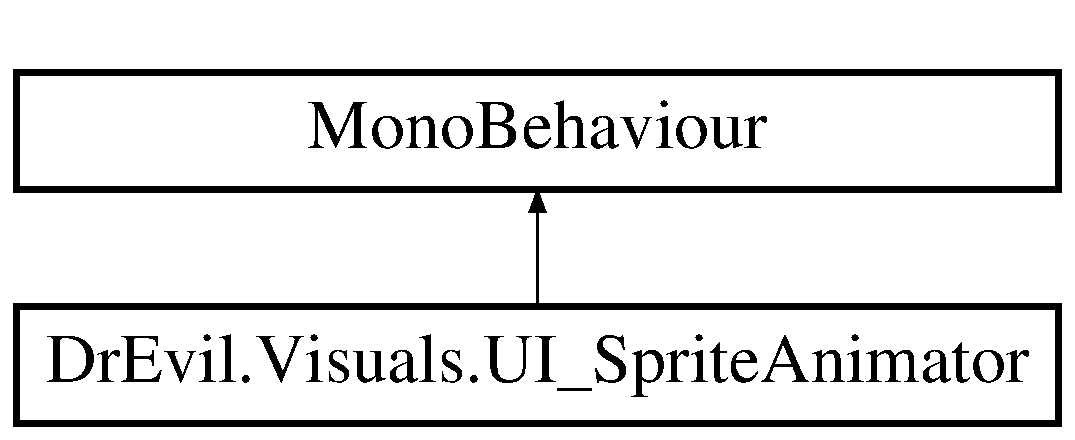
\includegraphics[height=2.000000cm]{class_dr_evil_1_1_visuals_1_1_u_i___sprite_animator}
\end{center}
\end{figure}
\subsection*{Public Member Functions}
\begin{DoxyCompactItemize}
\item 
I\+Enumerator \mbox{\hyperlink{class_dr_evil_1_1_visuals_1_1_u_i___sprite_animator_abe0f4c138486d258edf5c55c3ae5e797}{Start\+Animate}} ()
\begin{DoxyCompactList}\small\item\em Start to animate the sprite \end{DoxyCompactList}\item 
void \mbox{\hyperlink{class_dr_evil_1_1_visuals_1_1_u_i___sprite_animator_a5a8be113a9d81c7f98526d04bd7784ad}{Play\+One\+Burst\+With\+Callback}} (Action callback\+Action)
\begin{DoxyCompactList}\small\item\em Play Animation once and then Invoke cal\+Back\+Action \end{DoxyCompactList}\end{DoxyCompactItemize}
\subsection*{Public Attributes}
\begin{DoxyCompactItemize}
\item 
\mbox{\Hypertarget{class_dr_evil_1_1_visuals_1_1_u_i___sprite_animator_af83bc57079e687a798492ed3acabe703}\label{class_dr_evil_1_1_visuals_1_1_u_i___sprite_animator_af83bc57079e687a798492ed3acabe703}} 
Sprite \mbox{[}$\,$\mbox{]} {\bfseries sprites}
\item 
\mbox{\Hypertarget{class_dr_evil_1_1_visuals_1_1_u_i___sprite_animator_afc2b853953d81cefef02a2d57a05ded9}\label{class_dr_evil_1_1_visuals_1_1_u_i___sprite_animator_afc2b853953d81cefef02a2d57a05ded9}} 
float {\bfseries animation\+Speed}
\item 
\mbox{\Hypertarget{class_dr_evil_1_1_visuals_1_1_u_i___sprite_animator_a6a2bb7f3120255a10db3ed17cd33f9a7}\label{class_dr_evil_1_1_visuals_1_1_u_i___sprite_animator_a6a2bb7f3120255a10db3ed17cd33f9a7}} 
bool {\bfseries Play\+Once} = false
\item 
\mbox{\Hypertarget{class_dr_evil_1_1_visuals_1_1_u_i___sprite_animator_abae217ef4918306a6a023bcbf75e75b9}\label{class_dr_evil_1_1_visuals_1_1_u_i___sprite_animator_abae217ef4918306a6a023bcbf75e75b9}} 
bool {\bfseries Play\+On\+Enable} = true
\end{DoxyCompactItemize}


\subsection{Detailed Description}
Simple class for handling animations in U\+I-\/\+Canvas 



\subsection{Member Function Documentation}
\mbox{\Hypertarget{class_dr_evil_1_1_visuals_1_1_u_i___sprite_animator_a5a8be113a9d81c7f98526d04bd7784ad}\label{class_dr_evil_1_1_visuals_1_1_u_i___sprite_animator_a5a8be113a9d81c7f98526d04bd7784ad}} 
\index{Dr\+Evil\+::\+Visuals\+::\+U\+I\+\_\+\+Sprite\+Animator@{Dr\+Evil\+::\+Visuals\+::\+U\+I\+\_\+\+Sprite\+Animator}!Play\+One\+Burst\+With\+Callback@{Play\+One\+Burst\+With\+Callback}}
\index{Play\+One\+Burst\+With\+Callback@{Play\+One\+Burst\+With\+Callback}!Dr\+Evil\+::\+Visuals\+::\+U\+I\+\_\+\+Sprite\+Animator@{Dr\+Evil\+::\+Visuals\+::\+U\+I\+\_\+\+Sprite\+Animator}}
\subsubsection{\texorpdfstring{Play\+One\+Burst\+With\+Callback()}{PlayOneBurstWithCallback()}}
{\footnotesize\ttfamily void Dr\+Evil.\+Visuals.\+U\+I\+\_\+\+Sprite\+Animator.\+Play\+One\+Burst\+With\+Callback (\begin{DoxyParamCaption}\item[{Action}]{callback\+Action }\end{DoxyParamCaption})\hspace{0.3cm}{\ttfamily [inline]}}



Play Animation once and then Invoke cal\+Back\+Action 


\begin{DoxyParams}{Parameters}
{\em callback\+Action} & \\
\hline
\end{DoxyParams}
\mbox{\Hypertarget{class_dr_evil_1_1_visuals_1_1_u_i___sprite_animator_abe0f4c138486d258edf5c55c3ae5e797}\label{class_dr_evil_1_1_visuals_1_1_u_i___sprite_animator_abe0f4c138486d258edf5c55c3ae5e797}} 
\index{Dr\+Evil\+::\+Visuals\+::\+U\+I\+\_\+\+Sprite\+Animator@{Dr\+Evil\+::\+Visuals\+::\+U\+I\+\_\+\+Sprite\+Animator}!Start\+Animate@{Start\+Animate}}
\index{Start\+Animate@{Start\+Animate}!Dr\+Evil\+::\+Visuals\+::\+U\+I\+\_\+\+Sprite\+Animator@{Dr\+Evil\+::\+Visuals\+::\+U\+I\+\_\+\+Sprite\+Animator}}
\subsubsection{\texorpdfstring{Start\+Animate()}{StartAnimate()}}
{\footnotesize\ttfamily I\+Enumerator Dr\+Evil.\+Visuals.\+U\+I\+\_\+\+Sprite\+Animator.\+Start\+Animate (\begin{DoxyParamCaption}{ }\end{DoxyParamCaption})\hspace{0.3cm}{\ttfamily [inline]}}



Start to animate the sprite 

\begin{DoxyReturn}{Returns}

\end{DoxyReturn}


The documentation for this class was generated from the following file\+:\begin{DoxyCompactItemize}
\item 
Gamejam\+Unity/\+Assets/\+Scripts/U\+I\+\_\+\+Sprite\+Animator.\+cs\end{DoxyCompactItemize}

\hypertarget{class_dr_evil_1_1_visuals_1_1_u_i___text___rescaler}{}\section{Dr\+Evil.\+Visuals.\+U\+I\+\_\+\+Text\+\_\+\+Rescaler Class Reference}
\label{class_dr_evil_1_1_visuals_1_1_u_i___text___rescaler}\index{Dr\+Evil.\+Visuals.\+U\+I\+\_\+\+Text\+\_\+\+Rescaler@{Dr\+Evil.\+Visuals.\+U\+I\+\_\+\+Text\+\_\+\+Rescaler}}


Simple class to rescale text font size depending on screen size  


Inheritance diagram for Dr\+Evil.\+Visuals.\+U\+I\+\_\+\+Text\+\_\+\+Rescaler\+:\begin{figure}[H]
\begin{center}
\leavevmode
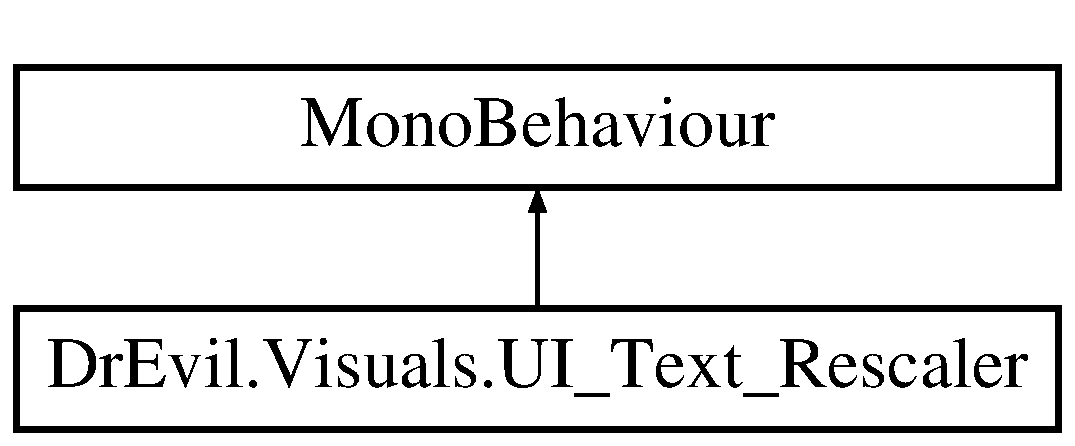
\includegraphics[height=2.000000cm]{class_dr_evil_1_1_visuals_1_1_u_i___text___rescaler}
\end{center}
\end{figure}
\subsection*{Public Member Functions}
\begin{DoxyCompactItemize}
\item 
\mbox{\Hypertarget{class_dr_evil_1_1_visuals_1_1_u_i___text___rescaler_a611b78cc6febe907045caa567a3d045e}\label{class_dr_evil_1_1_visuals_1_1_u_i___text___rescaler_a611b78cc6febe907045caa567a3d045e}} 
void {\bfseries Init} ()
\item 
\mbox{\Hypertarget{class_dr_evil_1_1_visuals_1_1_u_i___text___rescaler_ae22dbe89329ef5e26afe6c7d0ded92d8}\label{class_dr_evil_1_1_visuals_1_1_u_i___text___rescaler_ae22dbe89329ef5e26afe6c7d0ded92d8}} 
void {\bfseries Rescale\+Text\+Size} ()
\item 
\mbox{\Hypertarget{class_dr_evil_1_1_visuals_1_1_u_i___text___rescaler_a1b2199ad3c933760ec0a522bb9f1bfd0}\label{class_dr_evil_1_1_visuals_1_1_u_i___text___rescaler_a1b2199ad3c933760ec0a522bb9f1bfd0}} 
float {\bfseries Get\+Percentage\+Width} (float percentage)
\item 
\mbox{\Hypertarget{class_dr_evil_1_1_visuals_1_1_u_i___text___rescaler_ae6be95219435cd2147e5a2126e5a2cd8}\label{class_dr_evil_1_1_visuals_1_1_u_i___text___rescaler_ae6be95219435cd2147e5a2126e5a2cd8}} 
float {\bfseries Get\+Percentage\+Height} (float percentage)
\item 
void \mbox{\hyperlink{class_dr_evil_1_1_visuals_1_1_u_i___text___rescaler_a28595219a5b1654f56d4ad4b5a9ef663}{Apply\+All\+Resize\+Objs}} ()
\begin{DoxyCompactList}\small\item\em Apply all changes in all child objects \end{DoxyCompactList}\end{DoxyCompactItemize}
\subsection*{Public Attributes}
\begin{DoxyCompactItemize}
\item 
\mbox{\Hypertarget{class_dr_evil_1_1_visuals_1_1_u_i___text___rescaler_aefdb2e3c8f038b07fbc8611d34adf0c6}\label{class_dr_evil_1_1_visuals_1_1_u_i___text___rescaler_aefdb2e3c8f038b07fbc8611d34adf0c6}} 
float {\bfseries percentage\+Text\+Scale}
\item 
\mbox{\Hypertarget{class_dr_evil_1_1_visuals_1_1_u_i___text___rescaler_afeedadaa509e9943afaf474760966fb2}\label{class_dr_evil_1_1_visuals_1_1_u_i___text___rescaler_afeedadaa509e9943afaf474760966fb2}} 
bool {\bfseries is\+Magement\+Master}
\end{DoxyCompactItemize}


\subsection{Detailed Description}
Simple class to rescale text font size depending on screen size 



\subsection{Member Function Documentation}
\mbox{\Hypertarget{class_dr_evil_1_1_visuals_1_1_u_i___text___rescaler_a28595219a5b1654f56d4ad4b5a9ef663}\label{class_dr_evil_1_1_visuals_1_1_u_i___text___rescaler_a28595219a5b1654f56d4ad4b5a9ef663}} 
\index{Dr\+Evil\+::\+Visuals\+::\+U\+I\+\_\+\+Text\+\_\+\+Rescaler@{Dr\+Evil\+::\+Visuals\+::\+U\+I\+\_\+\+Text\+\_\+\+Rescaler}!Apply\+All\+Resize\+Objs@{Apply\+All\+Resize\+Objs}}
\index{Apply\+All\+Resize\+Objs@{Apply\+All\+Resize\+Objs}!Dr\+Evil\+::\+Visuals\+::\+U\+I\+\_\+\+Text\+\_\+\+Rescaler@{Dr\+Evil\+::\+Visuals\+::\+U\+I\+\_\+\+Text\+\_\+\+Rescaler}}
\subsubsection{\texorpdfstring{Apply\+All\+Resize\+Objs()}{ApplyAllResizeObjs()}}
{\footnotesize\ttfamily void Dr\+Evil.\+Visuals.\+U\+I\+\_\+\+Text\+\_\+\+Rescaler.\+Apply\+All\+Resize\+Objs (\begin{DoxyParamCaption}{ }\end{DoxyParamCaption})\hspace{0.3cm}{\ttfamily [inline]}}



Apply all changes in all child objects 



The documentation for this class was generated from the following file\+:\begin{DoxyCompactItemize}
\item 
Gamejam\+Unity/\+Assets/\+Scripts/U\+I\+\_\+\+Text\+\_\+\+Rescaler.\+cs\end{DoxyCompactItemize}

\hypertarget{class_world}{}\section{World Class Reference}
\label{class_world}\index{World@{World}}
\subsection*{Properties}
\begin{DoxyCompactItemize}
\item 
\mbox{\Hypertarget{class_world_a066b4282490f2481b2bb1502e24ff06a}\label{class_world_a066b4282490f2481b2bb1502e24ff06a}} 
string {\bfseries World\+Name}\hspace{0.3cm}{\ttfamily  \mbox{[}get, set\mbox{]}}
\item 
\mbox{\Hypertarget{class_world_a2180db73d20db8e635d6e380331fabe8}\label{class_world_a2180db73d20db8e635d6e380331fabe8}} 
List$<$ \mbox{\hyperlink{class_person}{Person}} $>$ {\bfseries Persons}\hspace{0.3cm}{\ttfamily  \mbox{[}get, set\mbox{]}}
\end{DoxyCompactItemize}


The documentation for this class was generated from the following file\+:\begin{DoxyCompactItemize}
\item 
Gamejam\+Unity/\+Assets/\+Scripts/\+Datastructure/Game\+World.\+cs\end{DoxyCompactItemize}

%--- End generated contents ---

% Index
\backmatter
\newpage
\phantomsection
\clearemptydoublepage
\addcontentsline{toc}{chapter}{Index}
\printindex

\end{document}
